\documentclass[12pt, a4paper]{book}
\begin{document}
\chapter{Network optimization}\label{chap:network_opt}
\section{Neural Network Training}
For most of the NN optimization methods we trained a NN with the following hyperparameters:
\begin{itemize}
   \item One hidden layer
   \item 100 neurons in the hidden layer
   \item 0.1 learning rate $\eta$
   \item $10^{-5}$ L2-regularization parameter $\lambda$
   \item The ADAM optimizer
\end{itemize}
We will mention whenever these parameters were not used. The results for the different network optimization methods explained in Chapter \ref{chap:NN_train} follow from here. Starting with the normalization of data.\\

\clearpage

\subsection{Normalization of data}\label{sec:normie_NN_res}
We trained a network using 80\% of the whole SM background events as well as 80\% of all the Z' DH HDS samples. As sample weights we only balanced the signal and background using the total number of simulated events, we did this by using method 3. on Chapter \ref{sec:balance_NN}, meaning that we weighed down the background with the ratio $\frac{N_{sig}}{N_{bkg}}$. 
We tested on the remaining 20\% of the SM background events, as well as 20\% of Z' DH HDS events where $m_{Z'} =130$ GeV. The different normalization methods explained in Chapter \ref{sec:normie_NN} have been tested and can be seen in the Figure \ref{fig:DifferentNormalizations}. 
To clarify the functioning of the validation plots, they illustrate the event distribution based on the ML algorithm score, ranging from 0 to 1, where a score of 1 signifies the ML algorithm's identification of the event as a Dark Matter (DM) signal event.
However, as we are conducting a supervised ML search we know whether an event is actually a DM signal event or an SM background event, using this we can plot the distributions of both cases to see how well the ML algorithm classifies signal from background. In the ideal case we would accumulate 
all signal events on the right side of the plot, and all background events on the left.\\
\\With the reminder of how the validation plots work, we can now discuss the results. From Figure \ref{fig:DifferentNormalizations} (a-c) we observe that the NN does a poor job at classifying signal from background. 
In fact, we get the best results in plot (d) and (e), with the Z-score method and Batch normalization. To study further which of these yield the best result for our search we can include real data points as well as uncertainties, 
as well as their calculate expected significance as explained in Chapter \ref{sec:siggy}, yields the plots shown in Figure \ref{fig:BestNormie}. For more Figures showing NN training results see the GitHub 
repo\footnote{Available here: \href{https://github.com/rubenguevara/Master-Thesis/tree/master/Plots/NeuralNetwork/Normalization_method}{https://github.com/rubenguevara/Master-Thesis/tree/master/\\Plots/NeuralNetwork/Normalization\_method}}. 
\graphicspath{{../../Plots/NeuralNetwork/Normalization_method/}}
\begin{figure}[!ht]
	\centering
	\begin{subfigure}[b]{0.49\textwidth}
      \centering
      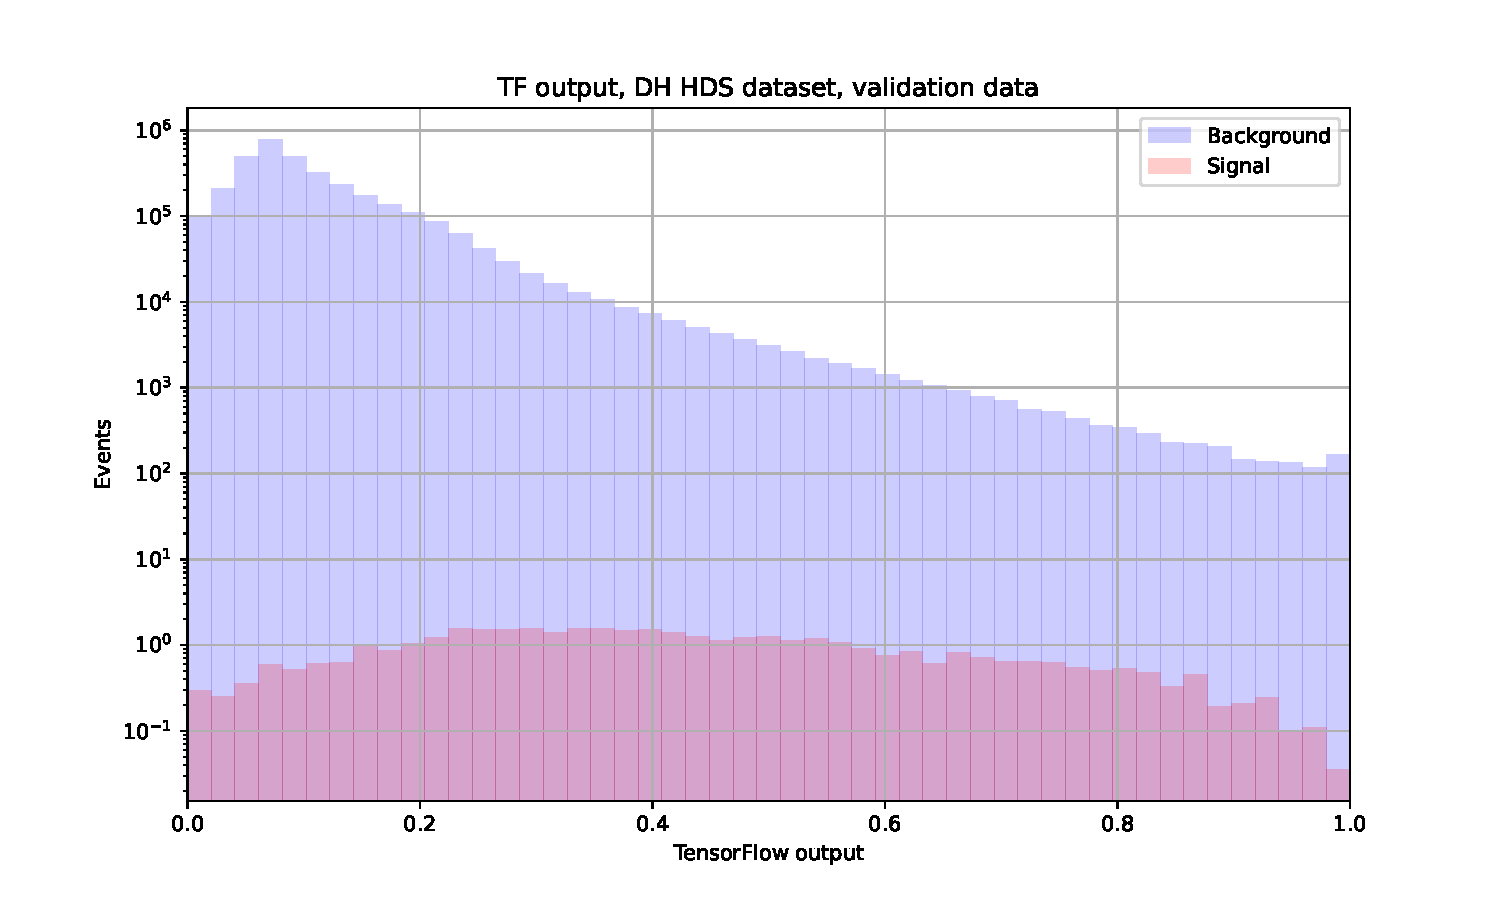
\includegraphics[width=1\textwidth]{NoNorm/VAL_pre.pdf}
      \caption{No normalization}
   \end{subfigure}
   \hfill
   \begin{subfigure}[b]{0.49\textwidth}
      \centering
      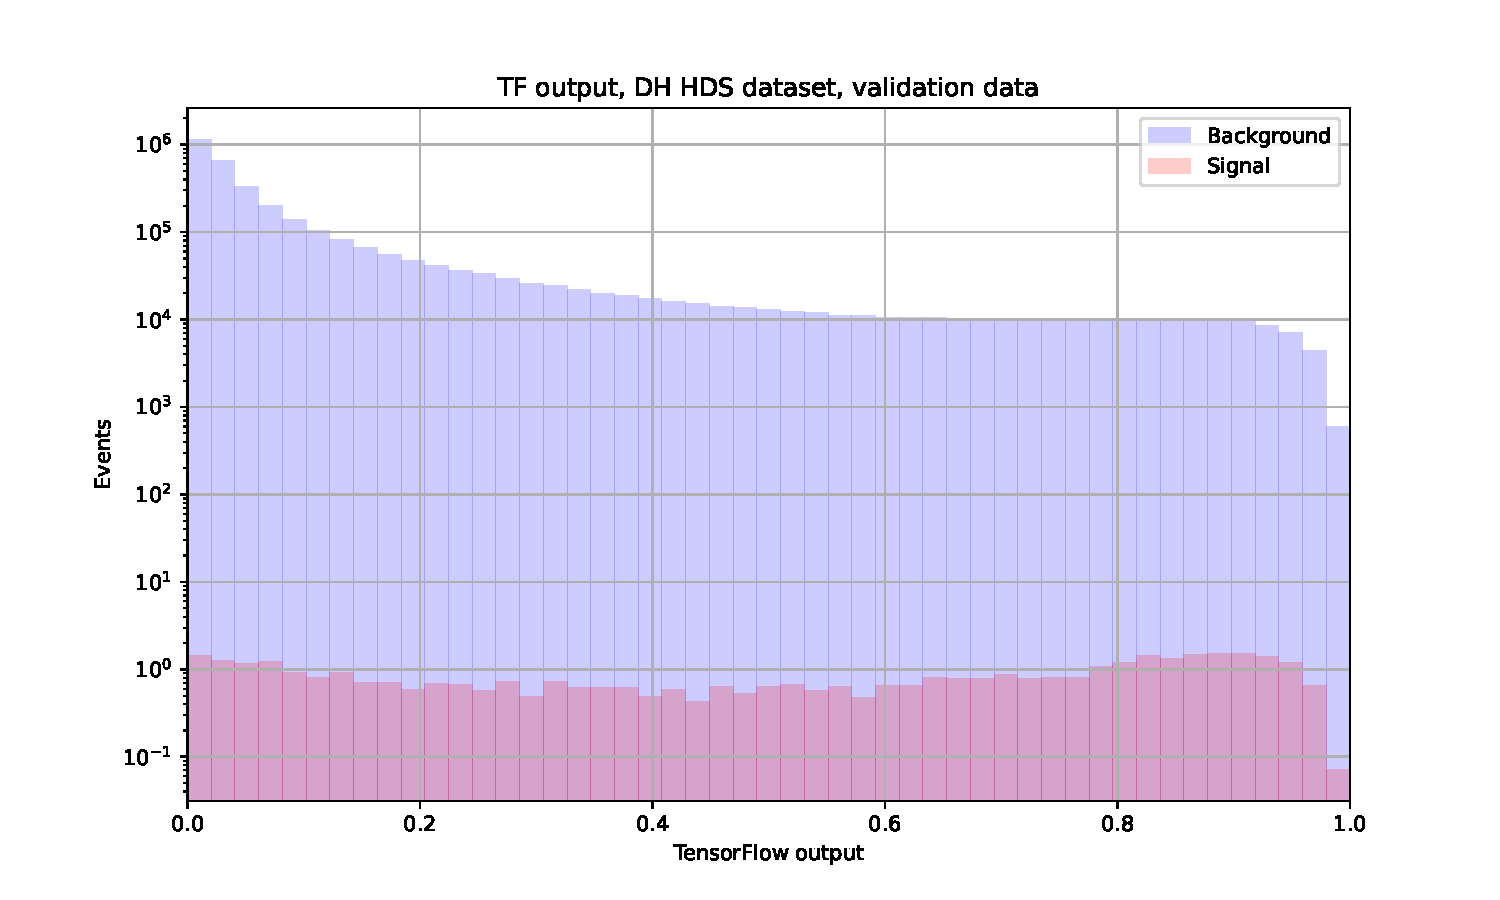
\includegraphics[width=1\textwidth]{LayerNorm/VAL_pre.pdf}
      \caption{Layer normalization}
   \end{subfigure}
   \hfill
	\begin{subfigure}[b]{0.49\textwidth}
      \centering
      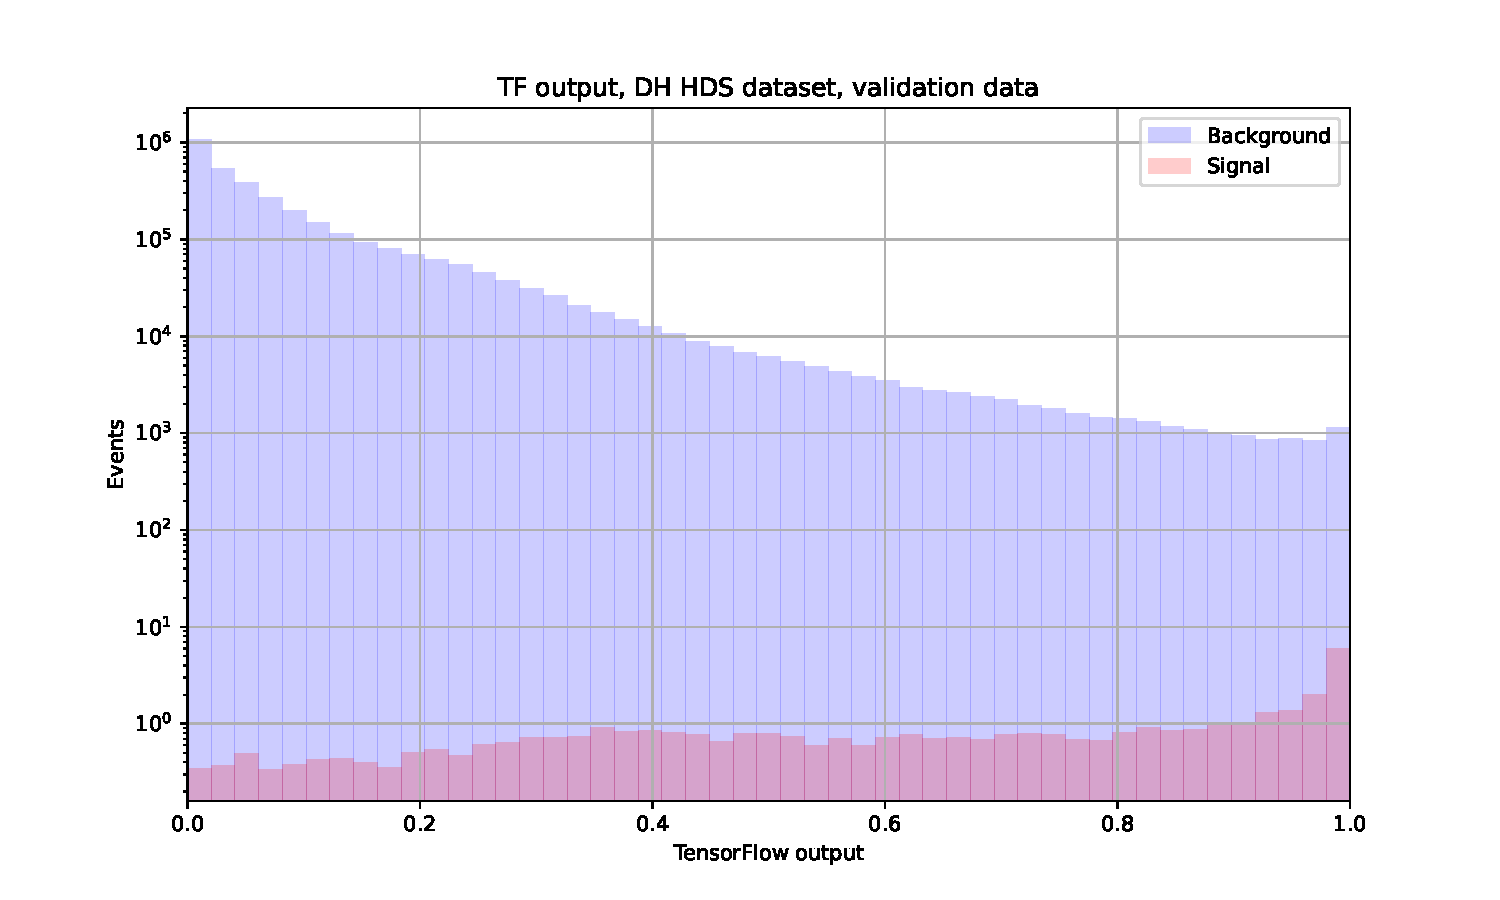
\includegraphics[width=1\textwidth]{minmax/VAL_pre.pdf}
      \caption{Min max scaling}
   \end{subfigure}
   \hfill
   \begin{subfigure}[b]{0.49\textwidth}
      \centering
      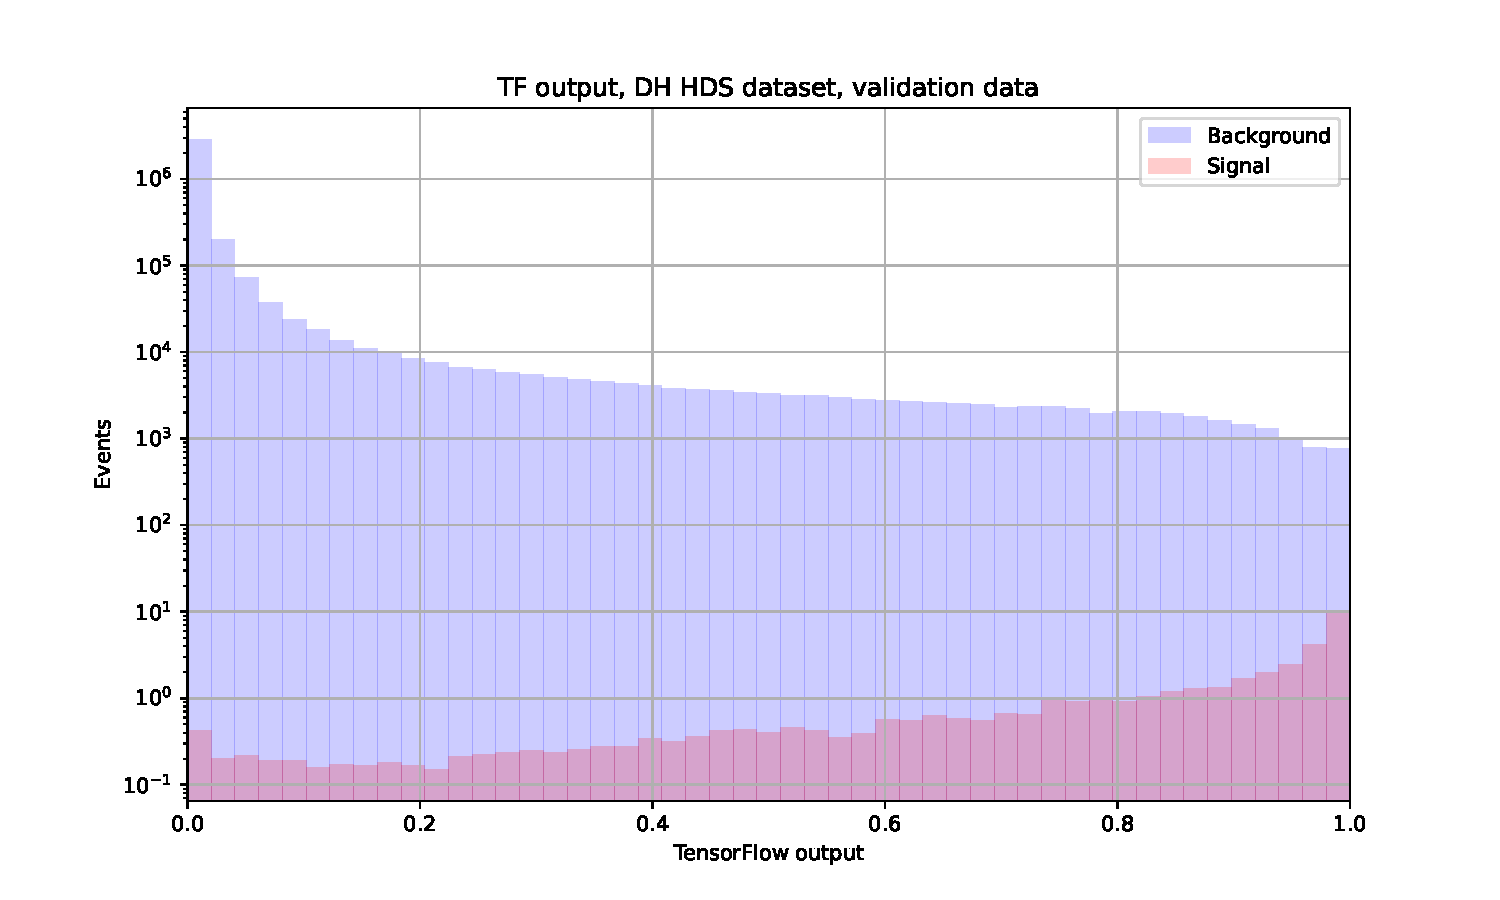
\includegraphics[width=1\textwidth]{Z_score/VAL_pre.pdf}
      \caption{Z-score}
   \end{subfigure}
   \hfill
   \begin{subfigure}[b]{0.49\textwidth}
      \centering
      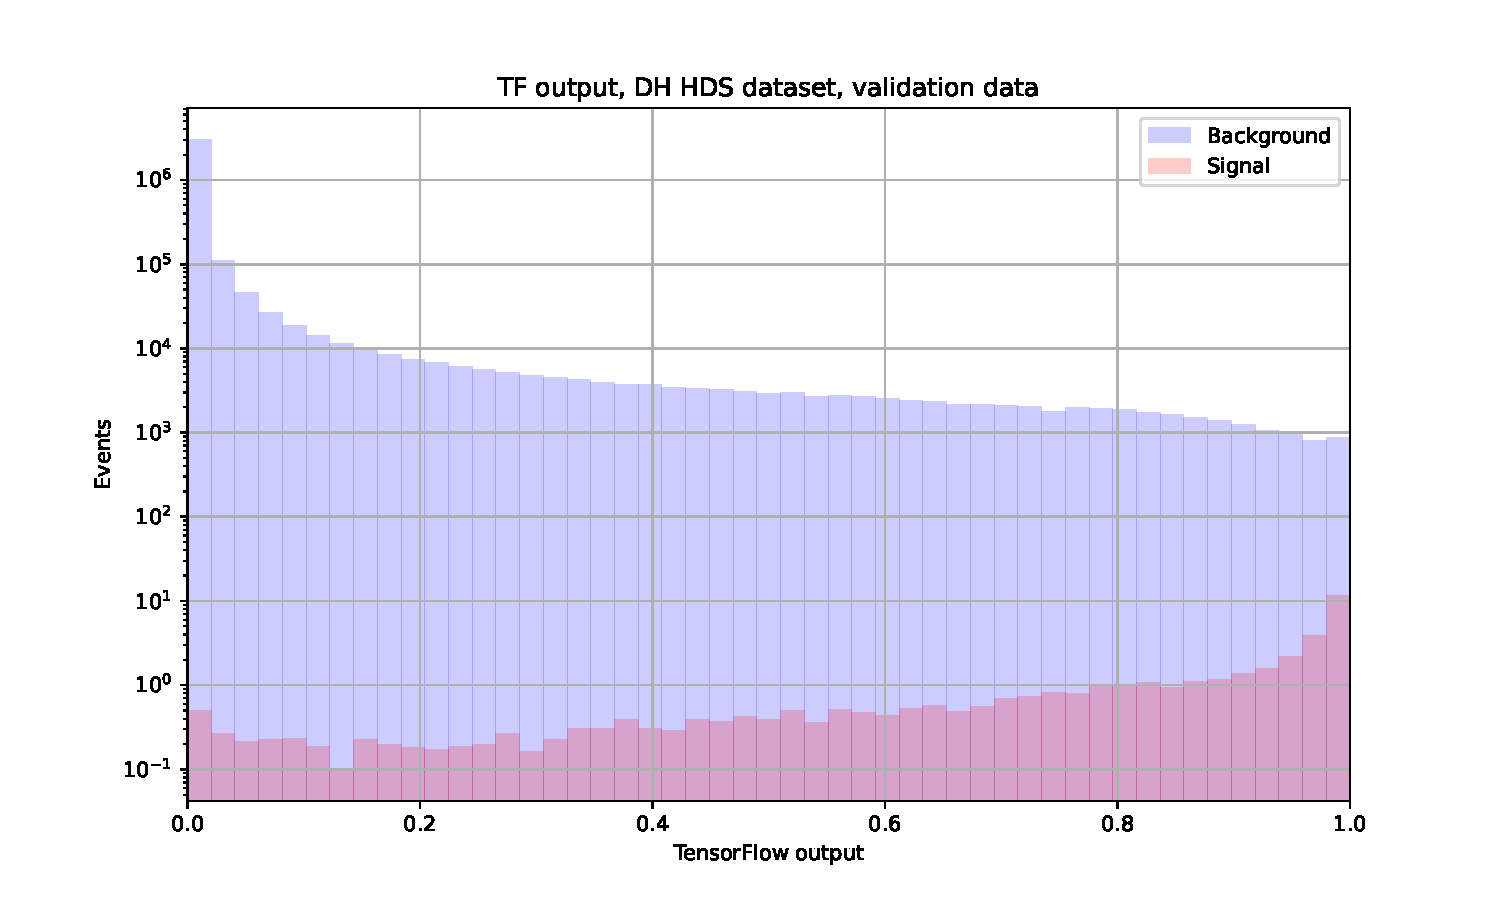
\includegraphics[width=1\textwidth]{BatchNorm/VAL_pre.pdf}
      \caption{Batch normalization}
   \end{subfigure}
   \caption[Different normalization methods for NNs]{NN prediction when using different normalization methods. This is testing a dataset with 20\% of the Z' DH HDS $m_{Z'}=130$ GeV events.}\label{fig:DifferentNormalizations}
\end{figure}
\clearpage
\begin{figure}[!ht]
	\centering
	\begin{subfigure}[b]{0.49\textwidth}
      \centering
      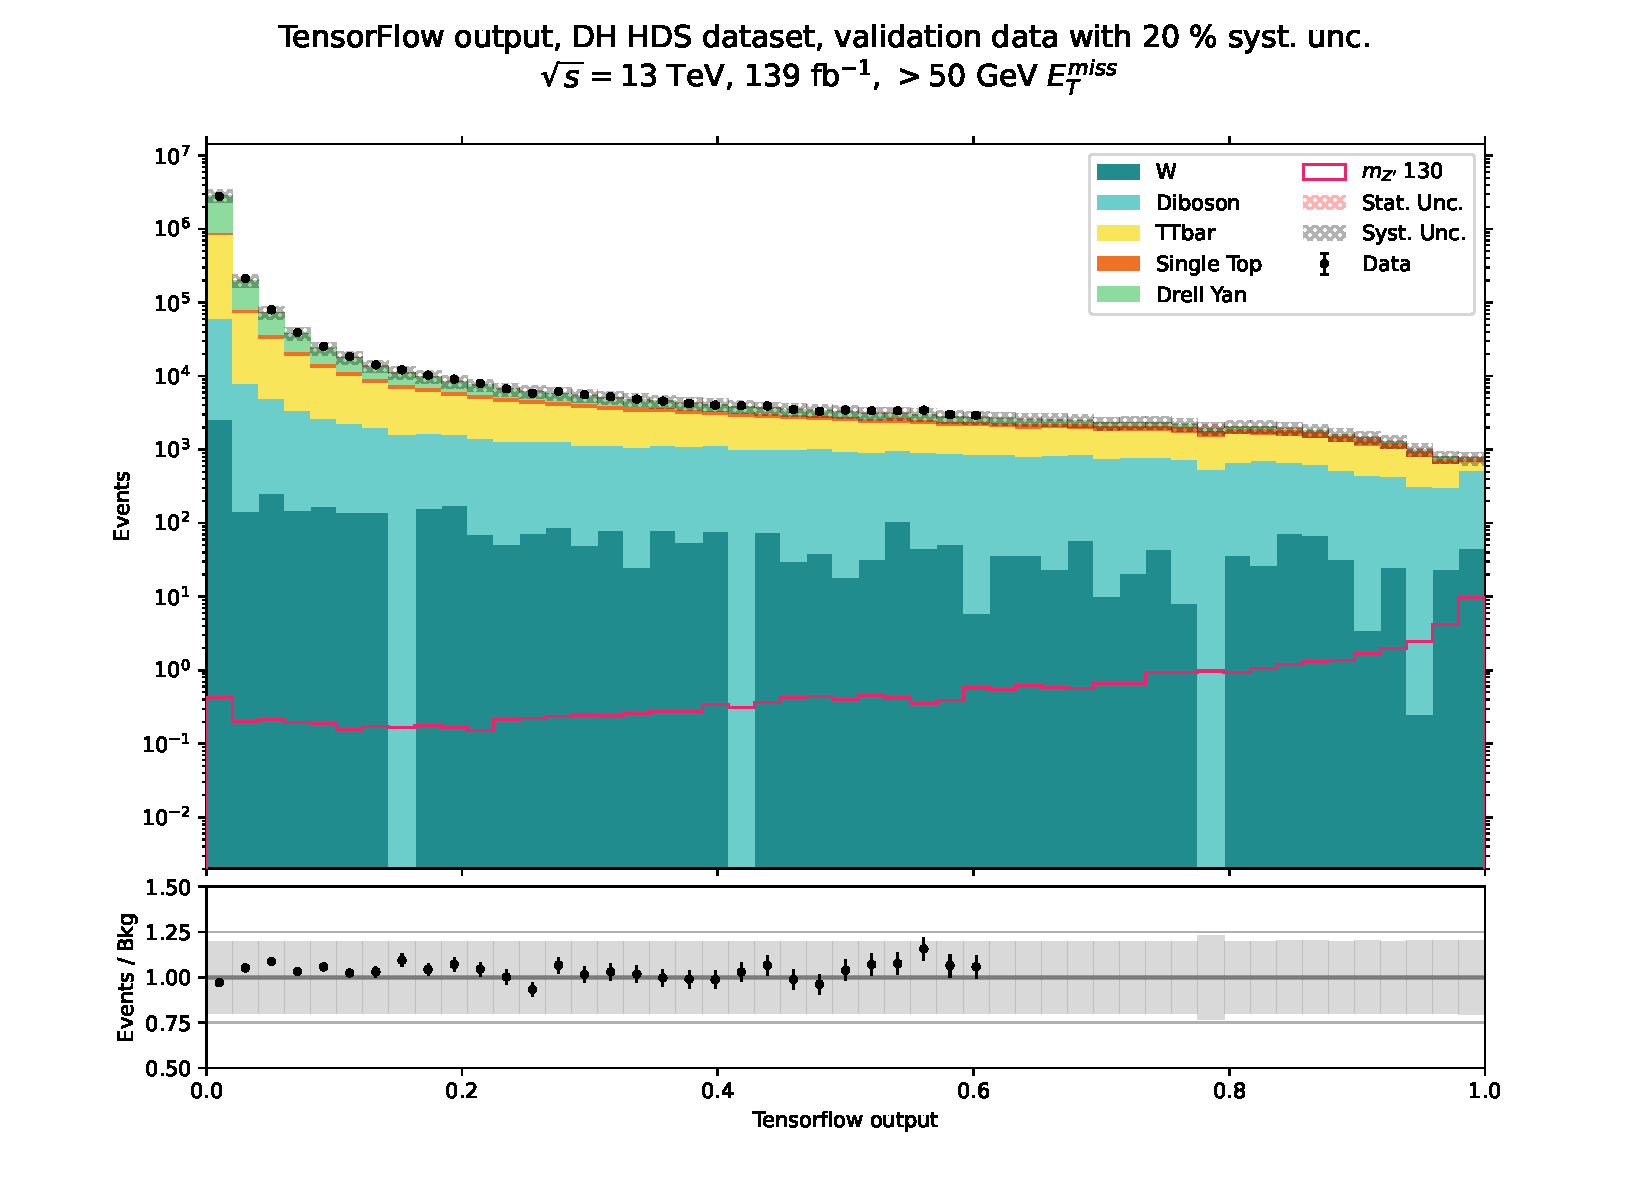
\includegraphics[width=1\textwidth]{Z_score/VAL.pdf}
      \caption{Z-score}
   \end{subfigure}
   \hfill
   \begin{subfigure}[b]{0.49\textwidth}
      \centering
      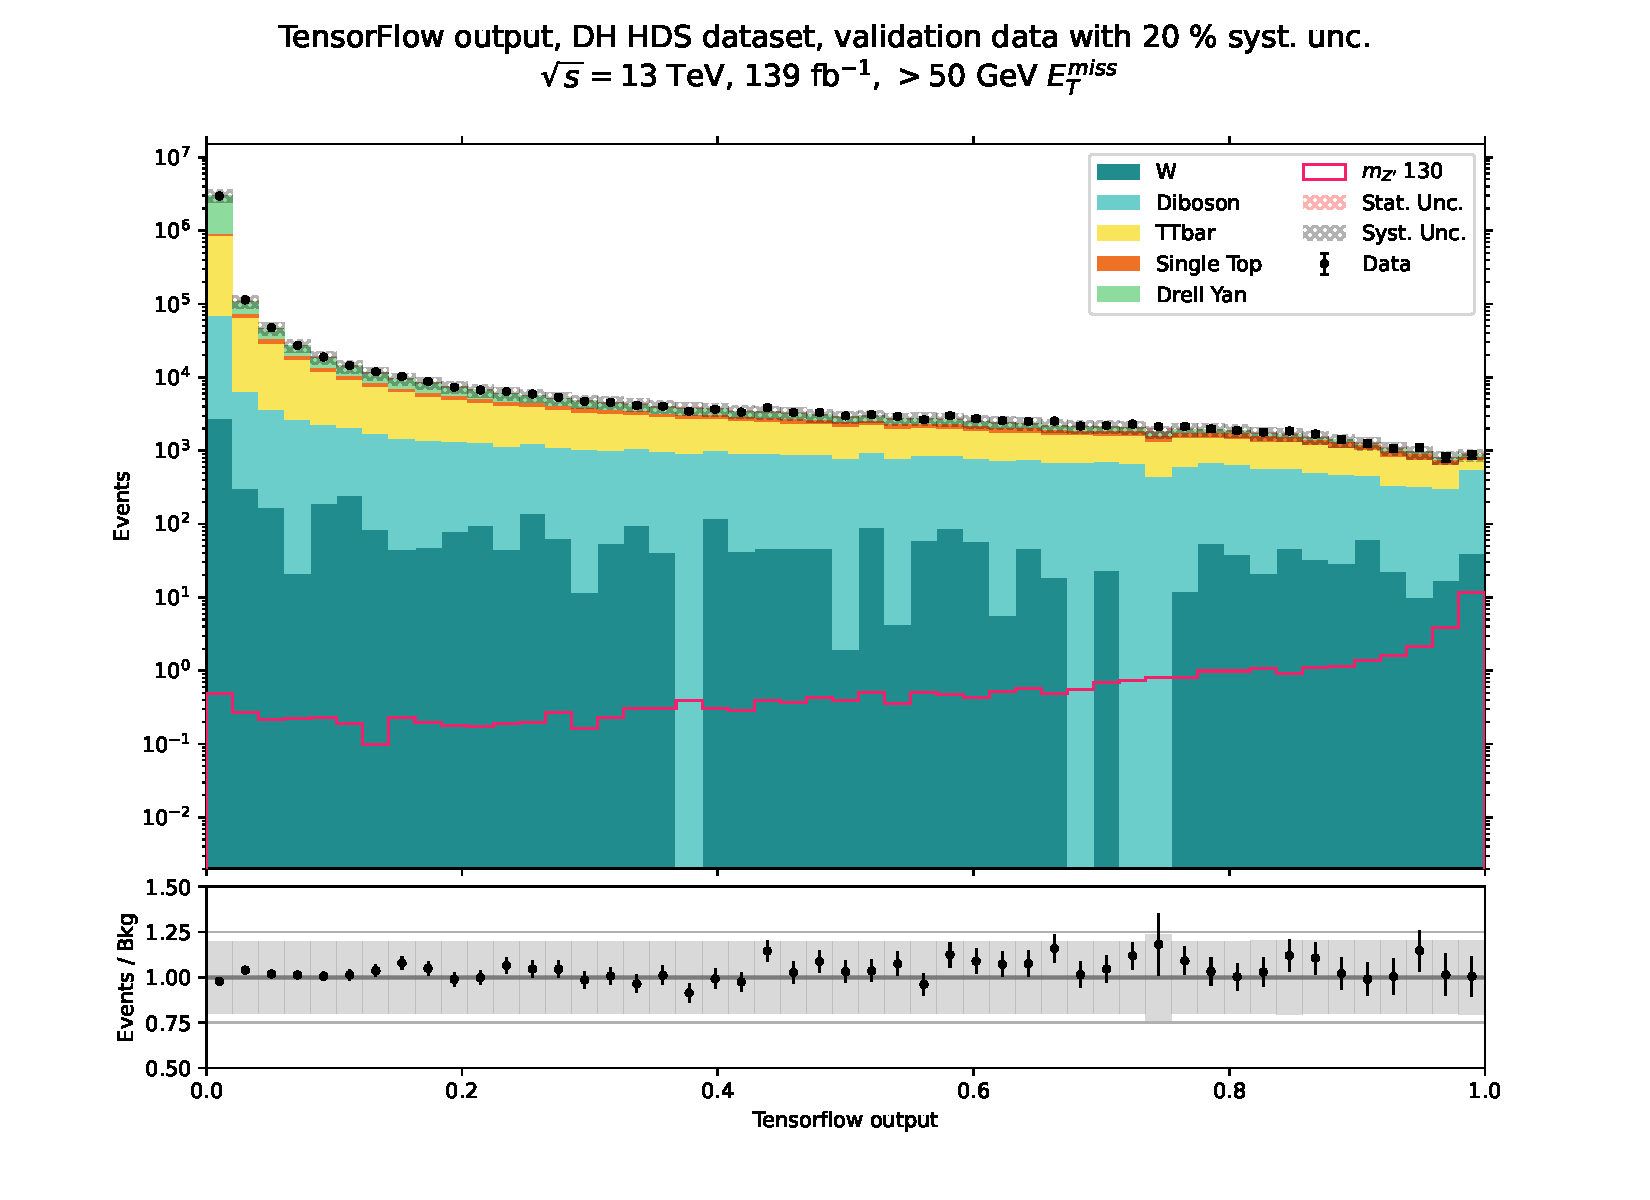
\includegraphics[width=1\textwidth]{BatchNorm/VAL.pdf}
      \caption{Batch normalization}
   \end{subfigure}
   \hfill
   \begin{subfigure}[b]{0.49\textwidth}
      \centering
      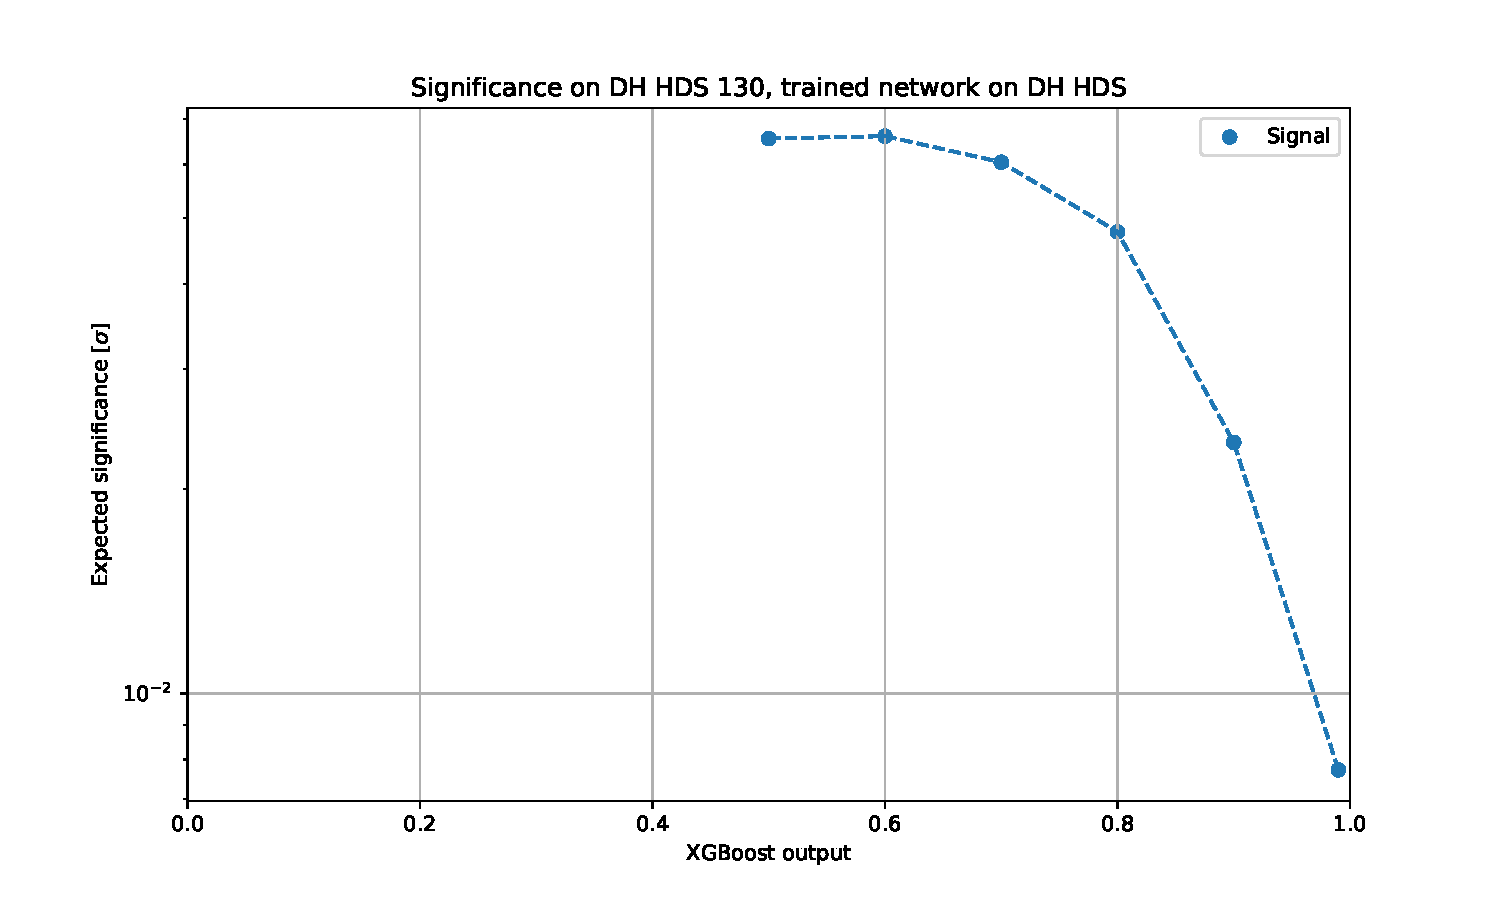
\includegraphics[width=1\textwidth]{Z_score/EXP_SIG.pdf}
      \caption{The expected significance of (a)}
   \end{subfigure}
   \hfill
   \begin{subfigure}[b]{0.49\textwidth}
      \centering
      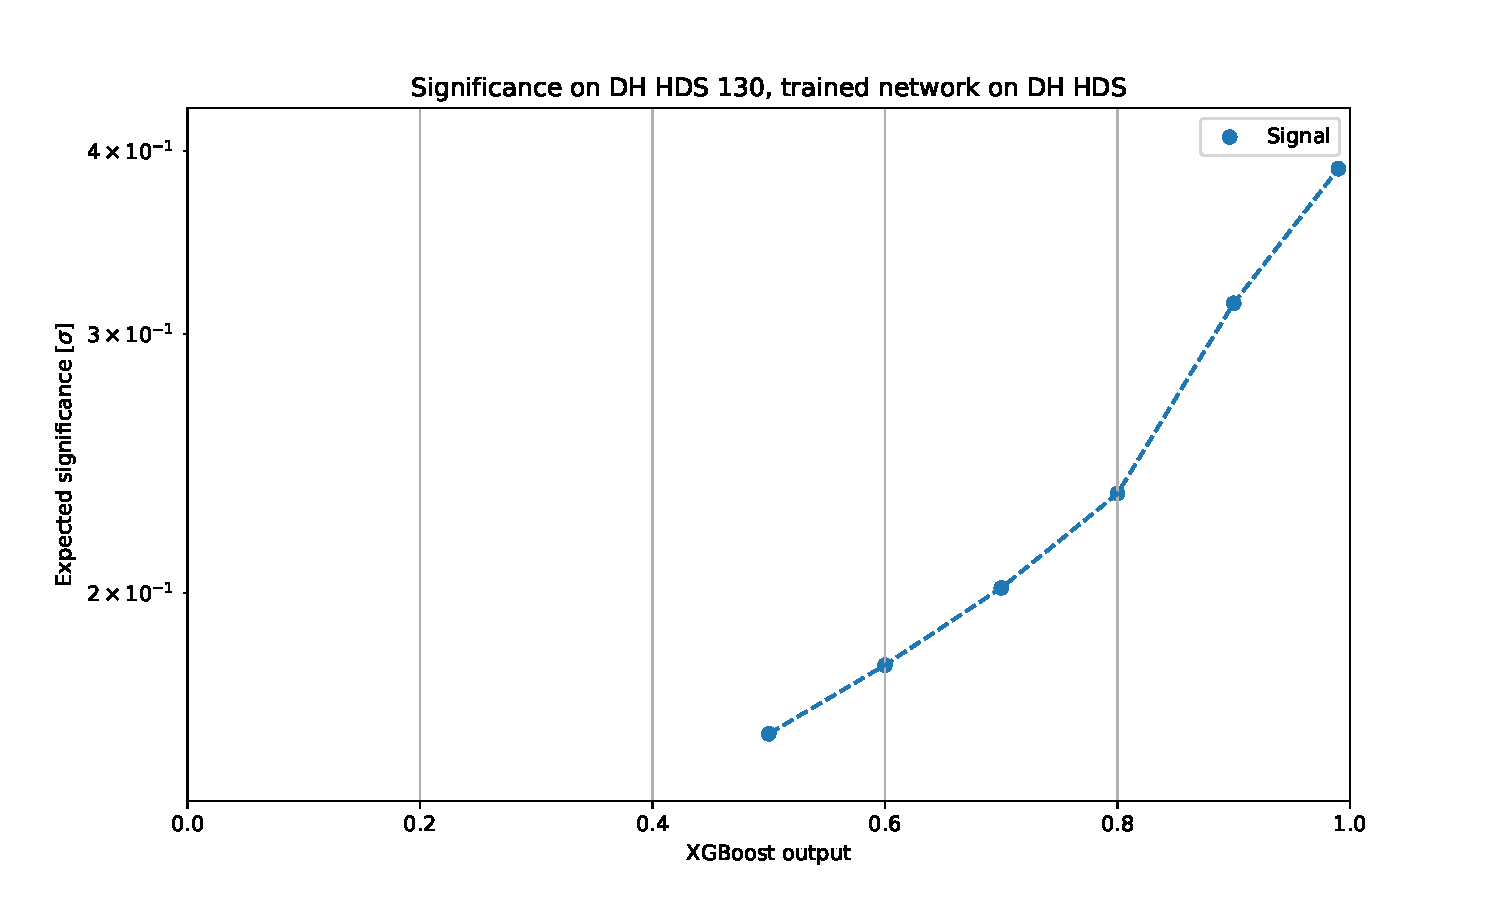
\includegraphics[width=1\textwidth]{BatchNorm/EXP_SIG.pdf}
      \caption{The expected significance of (b)}
   \end{subfigure}
   \caption[Comparison of best NN normalization methods and expected significance calculation]{Comparison of the best normalization methods. Figure (a) and (b) show the validation data of both cases, c) and d) show the expected significance of the validation plots when making a cut on the output. }\label{fig:BestNormie}
\end{figure}
\noindent In Figure \ref{fig:BestNormie} we can see the \verb|Batch_normalization| method gives us an overall higher value of expected significance, meaning that it is better at classifying signal from background. 
Because of this, and because it is easier to implement this normalization method, we will use this further in the NN optimization studies. 
\clearpage



\subsection{Balancing of signal and background}\label{sec:NN_balance_rst}
To try the different sample weight methods explained in Chapter \ref{sec:balance_NN} we used a dataset consisting of only SM events where the goal was to treat the $W$ channel as signal and try to isolate it from other SM processes, as the number of events for this background challenge resembles the data unbalance we have with some of our DM models. 
To train we used \verb|Batch_normalization| and 80\% of the SM background events. 
To test we used the remaining 20\% of SM events. We also tested the difference in performance when using the SGD and ADAM optimizers. The difference in distributions when using different optimizers can be seen in Figure \ref{fig:ADAMvsSGD}, here the balancing method (3. on Chapter \ref{sec:balance_NN}) is used.
\graphicspath{{../../Plots/NeuralNetwork/W/}} 
\begin{figure}[!ht]
	\centering
      \begin{subfigure}[b]{0.49\textwidth}
         \centering
         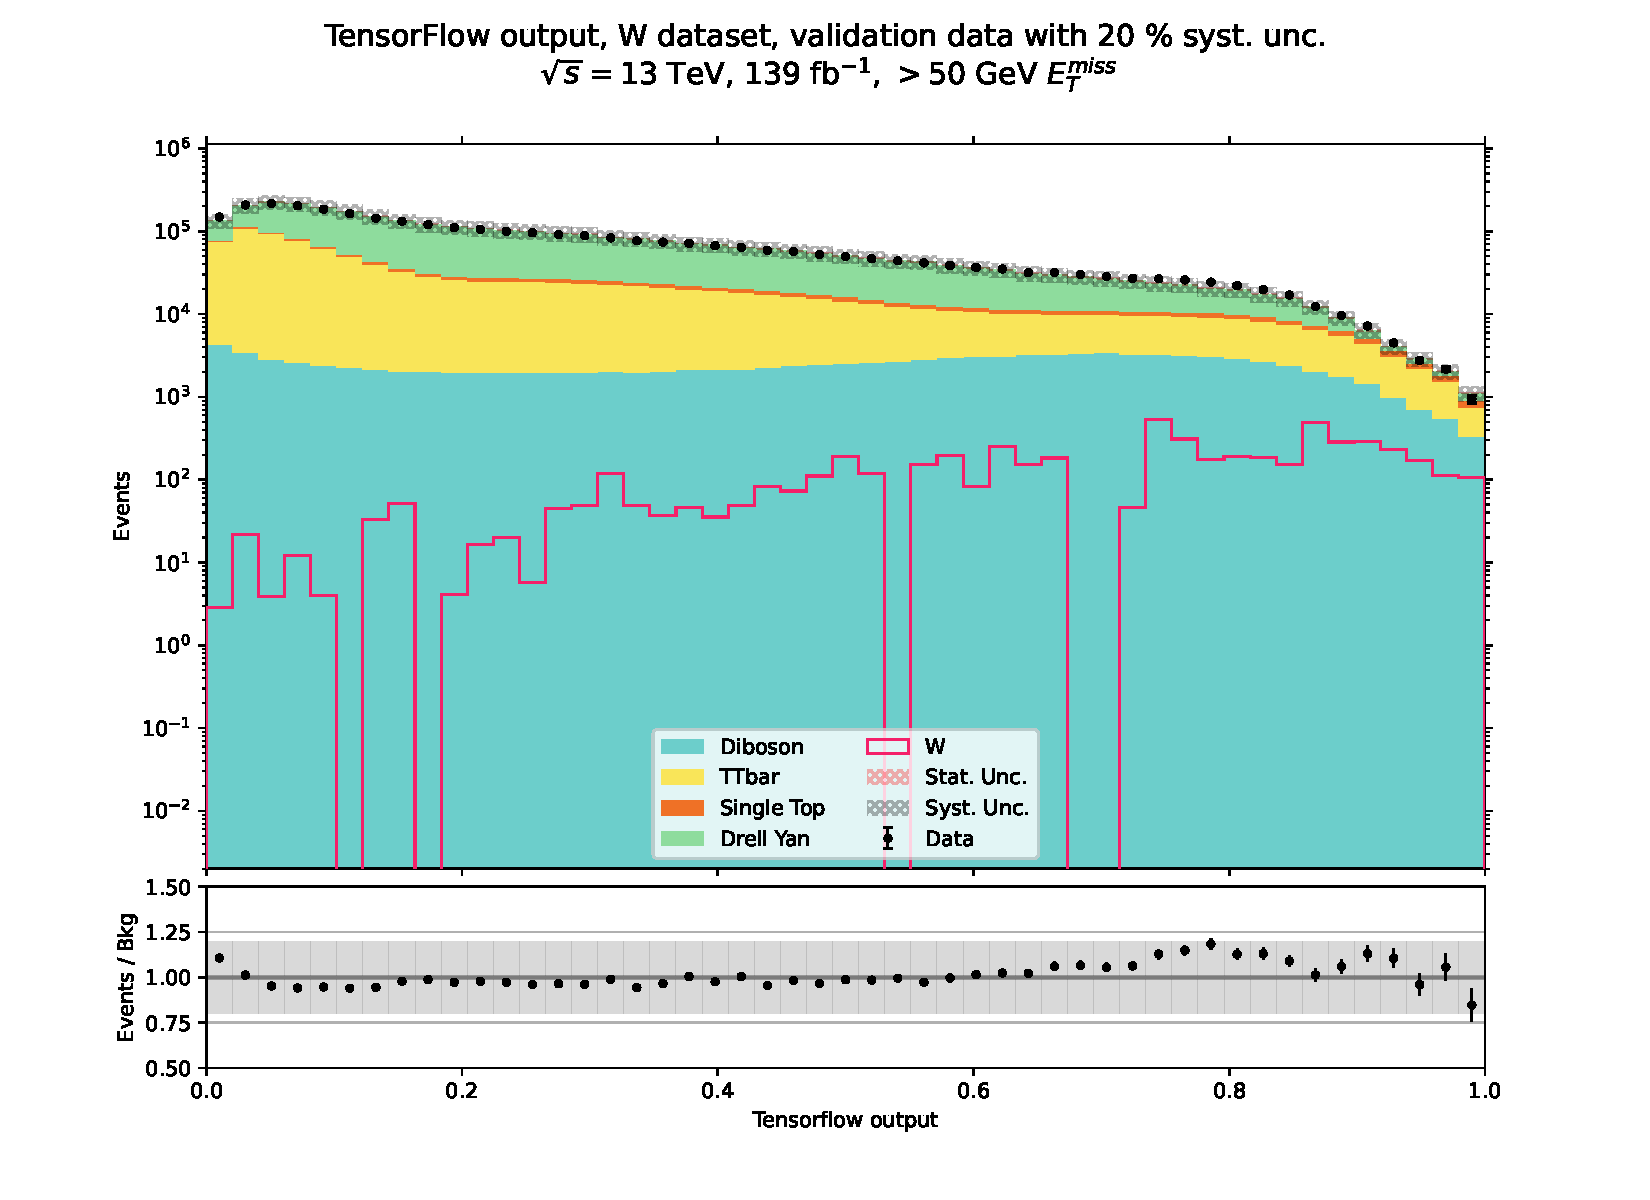
\includegraphics[width=1\textwidth]{Balanced/VAL.pdf}
         \caption{Using ADAM}
      \end{subfigure}
      \begin{subfigure}[b]{0.49\textwidth}
         \centering
         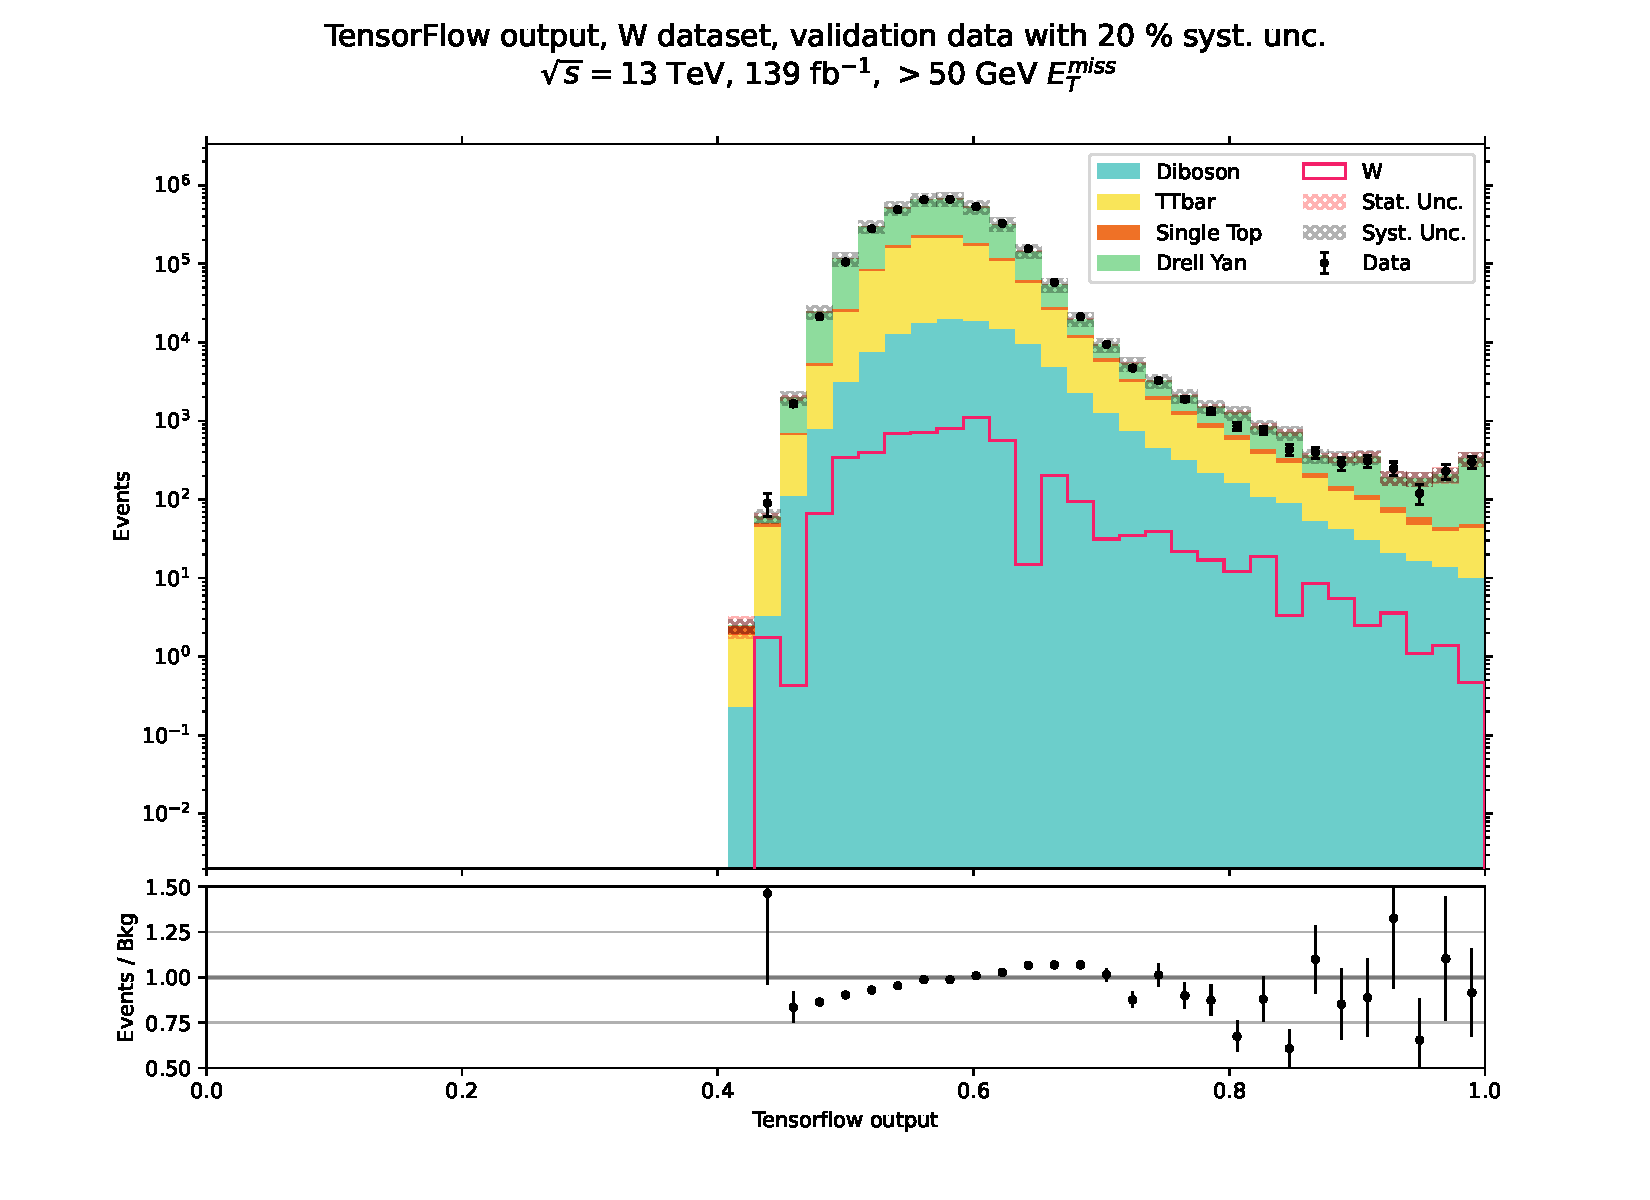
\includegraphics[width=1\textwidth]{SGD/Balanced/VAL.pdf}
         \caption{Using SGD}
      \end{subfigure}
      \caption[Difference between ADAM and SGD optimizer]{Validation plots using SGD and ADAM. 
      This was done using a dataset where the goal was to isolate the $W$ background process from other SM background processes}\label{fig:ADAMvsSGD}
\end{figure}
\\As ADAM is far better at sorting signal from background, since as we can see the ML algorithm using SGD gives a score of 0.5 or higher to every event, we will only use this optimizer further.\\
\\The results for the different weighting methods can be seen in Figure \ref{fig:WVAL}, which shows the validation plots and in Figure \ref{fig:WROC} which shows the ROC score. For more Figures showing NN training results see the GitHub repo\footnote{Available here: \href{https://github.com/rubenguevara/Master-Thesis/tree/master/Plots/NeuralNetwork/W}{https://github.com/rubenguevara/Master-Thesis/tree/master/\\Plots/NeuralNetwork/W}}. \\
\\As we can see from Figure \ref{fig:WVAL}, the only method where the NN is able to give a full distribution of output scores is the balancing method. If we do not balance the W signal from the rest of the SM background we see that 
the NN guesses all events to be background events (as the plots in (a) and (b) do not give a score higher than 0.5). The AUC-score of the balancing method is the highest, as seen Figure \ref{fig:WROC}, this supports that the balancing method is better with unbalanced datasets.  
\begin{figure}[!ht]
	\centering
	\begin{subfigure}[b]{0.49\textwidth}
         \centering
         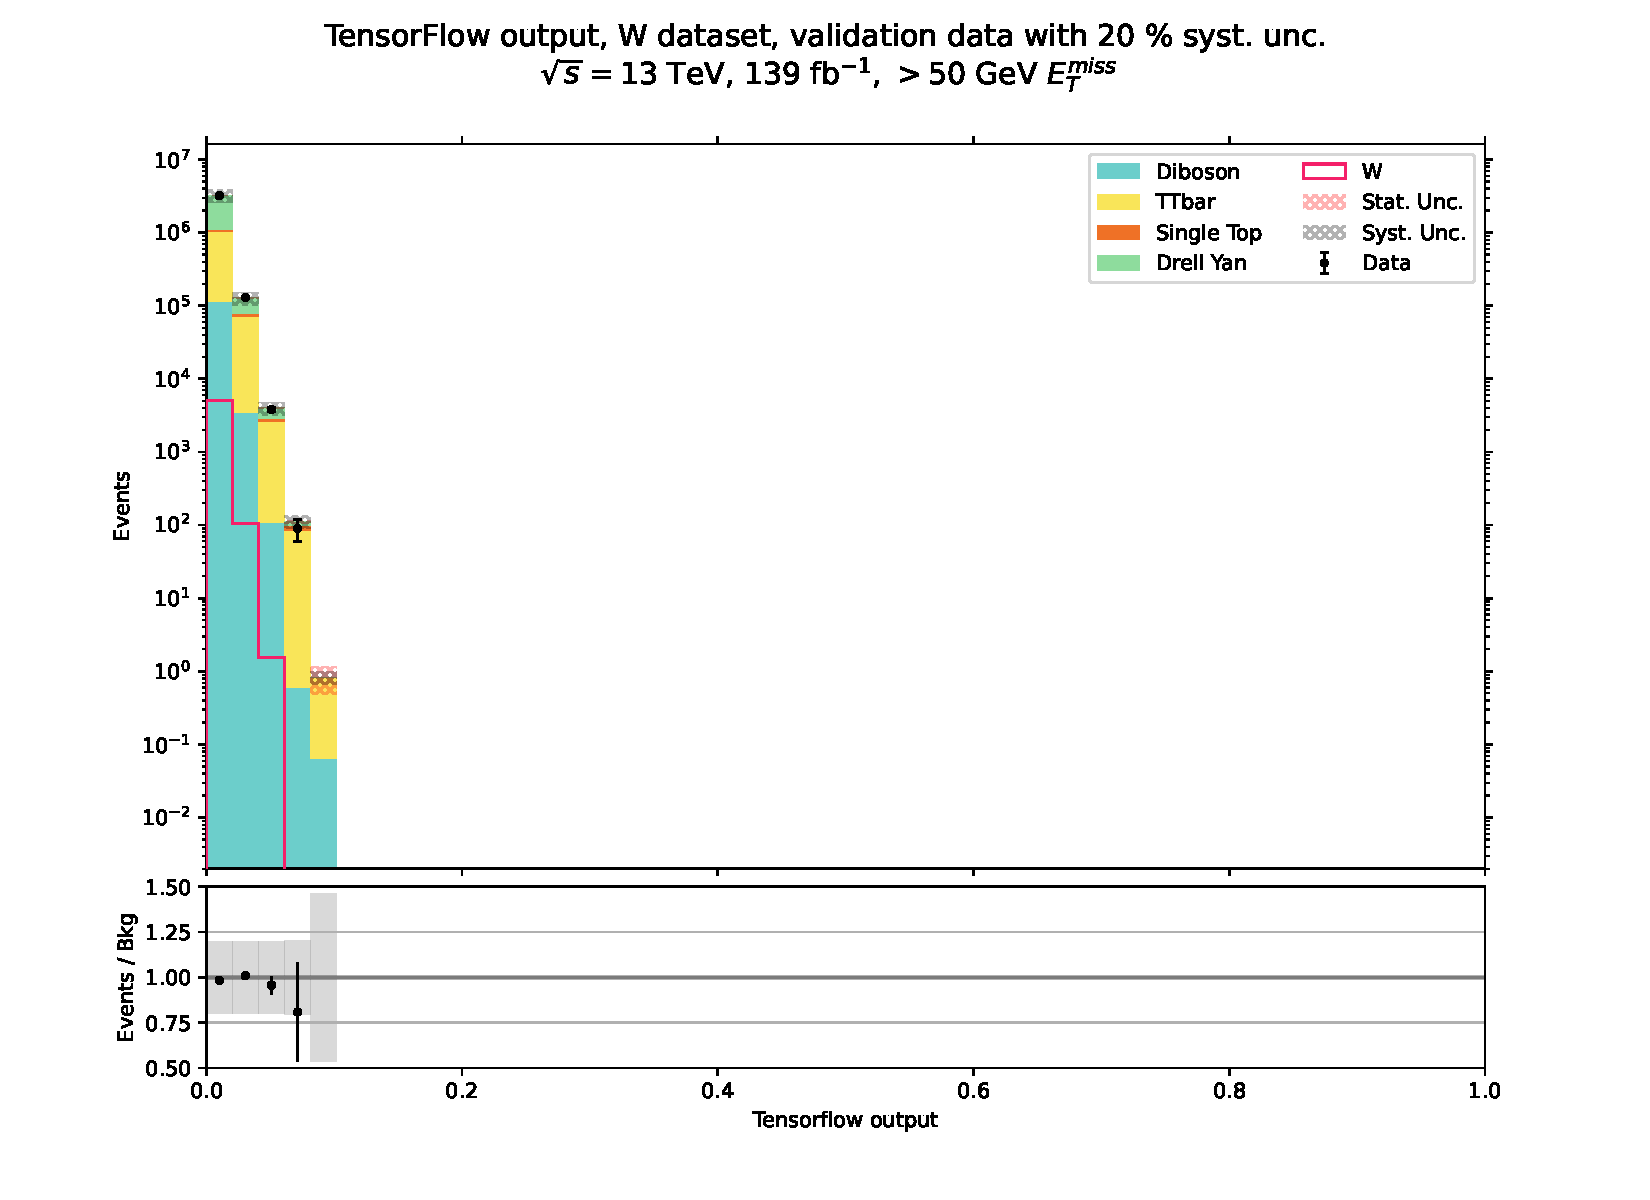
\includegraphics[width=1\textwidth]{Unweighted/VAL.pdf}
         \caption{Using no weights}\label{fig:WVALUW}
      \end{subfigure}
      \hfill
      \begin{subfigure}[b]{0.49\textwidth}
         \centering
         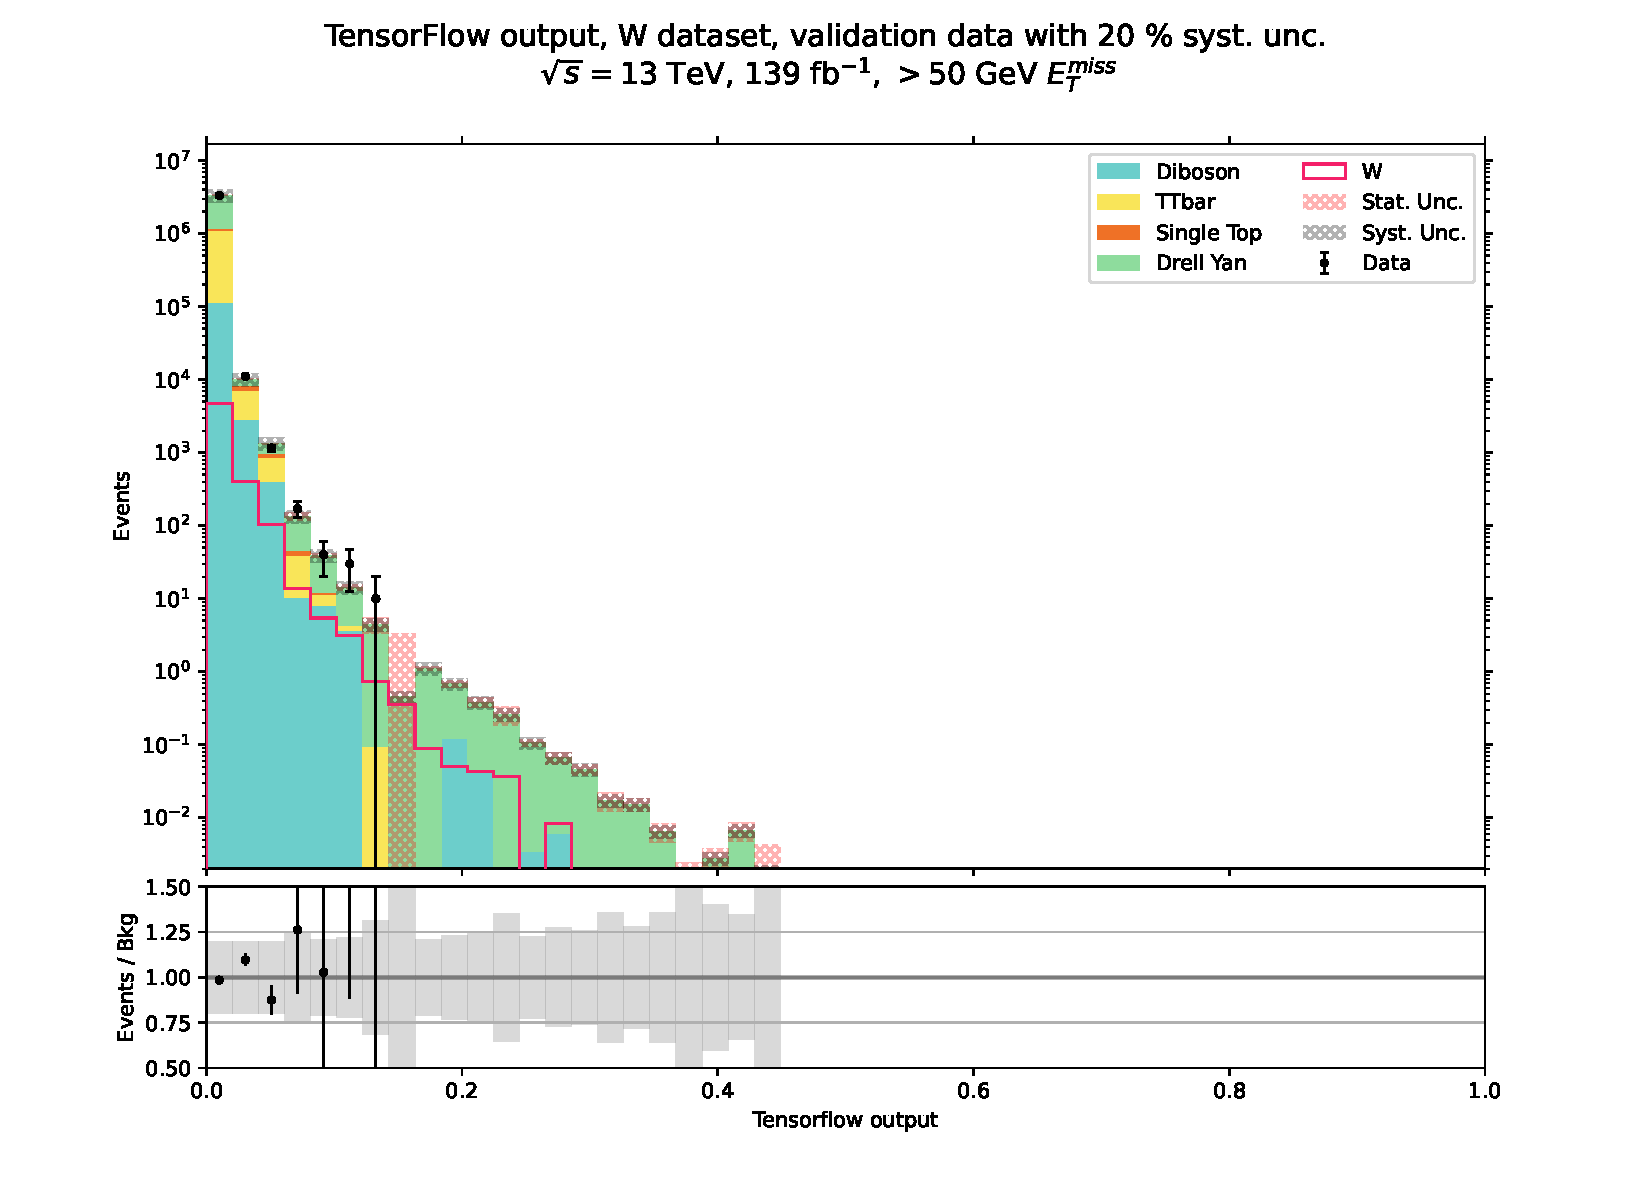
\includegraphics[width=1\textwidth]{Weighted/VAL.pdf}
         \caption{Using re-weighting weights}\label{fig:WVALMC}
      \end{subfigure}
      \begin{subfigure}[b]{0.49\textwidth}
         \centering
         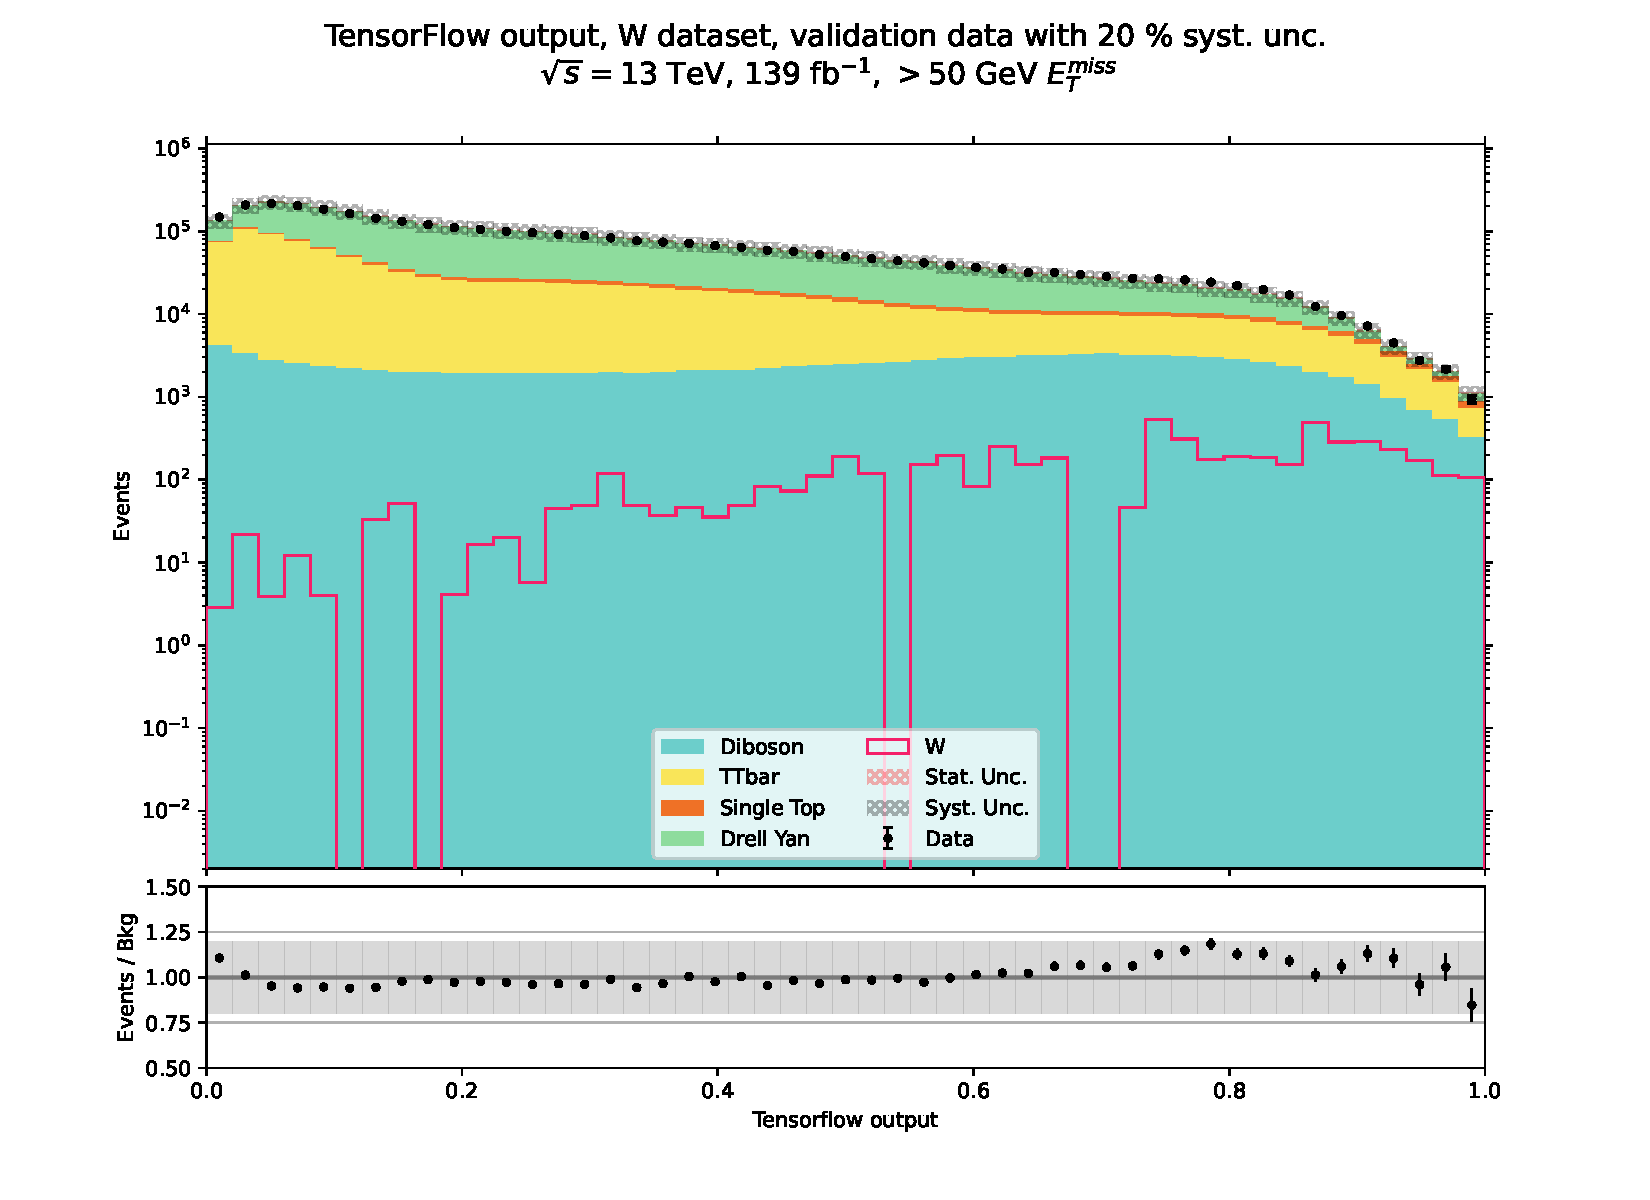
\includegraphics[width=1\textwidth]{Balanced/VAL.pdf}
         \caption{Using $\frac{N_{sig}}{N_{bkg}}$}\label{fig:WVALW}
      \end{subfigure}
      \caption[Validation plots for different balancing methods on NN]{Validation plots of different balancing methods. 
      This was done using a dataset where the goal was to isolate the $W$ background process from other SM background processes}\label{fig:WVAL}
\end{figure}
\begin{figure}[!ht]
	\centering
	\begin{subfigure}[b]{0.49\textwidth}
         \centering
         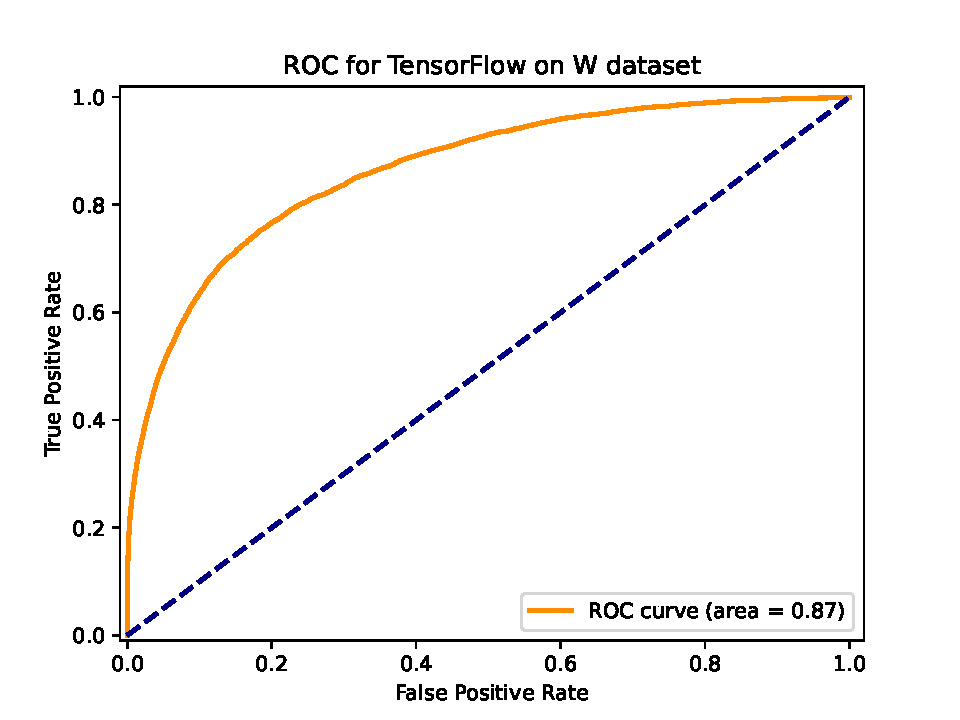
\includegraphics[width=1\textwidth]{Unweighted/ROC.pdf}
         \caption{Using no weights}\label{fig:WROCUW}
      \end{subfigure}
      \hfill
      \begin{subfigure}[b]{0.49\textwidth}
         \centering
         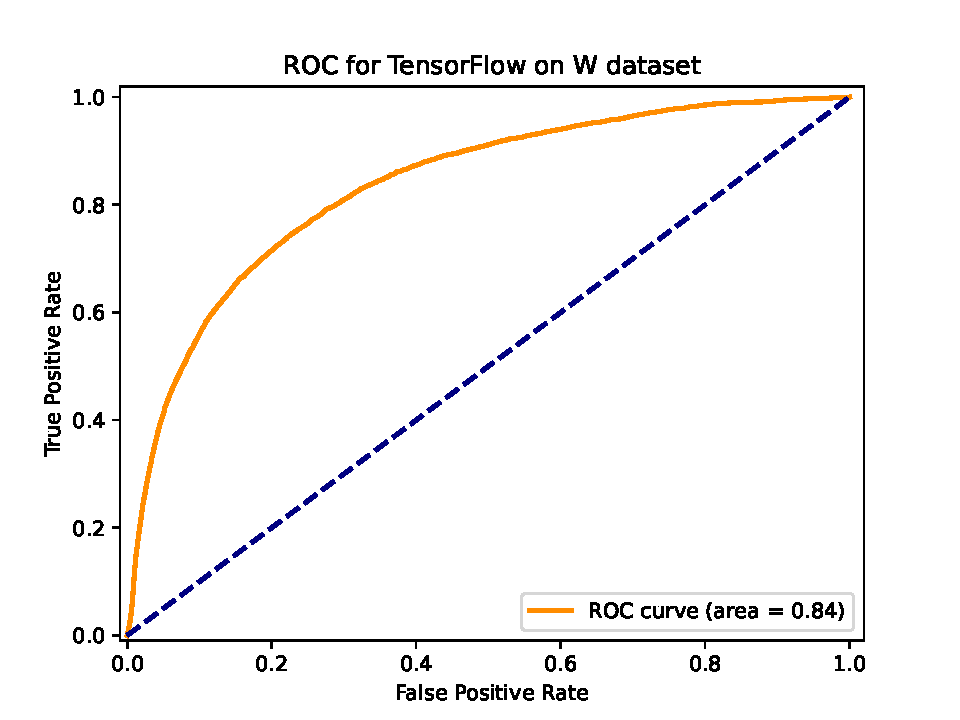
\includegraphics[width=1\textwidth]{Weighted/ROC.pdf}
         \caption{Using re-weighting weights}\label{fig:WROCMC}
      \end{subfigure}
      \begin{subfigure}[b]{0.49\textwidth}
         \centering
         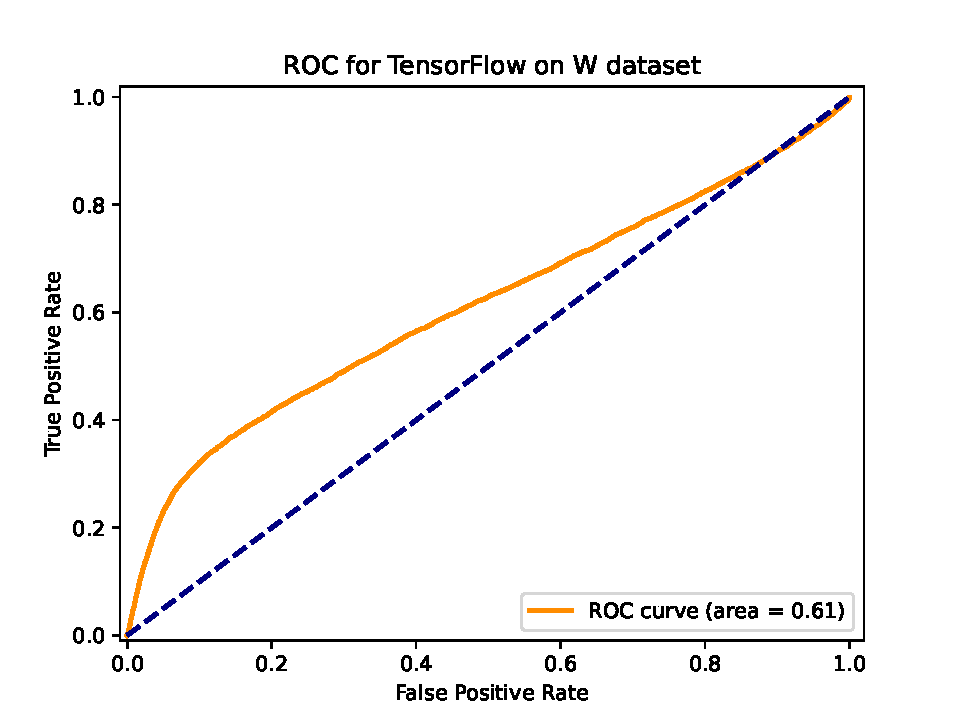
\includegraphics[width=1\textwidth]{Balanced/ROC.pdf}
         \caption{Using $\frac{N_{sig}}{N_{bkg}}$}\label{fig:WROCW}
      \end{subfigure}
      \caption[ROC plots for different balancing methods on NN]{ROC plots of different balancing methods. 
      This was done using a dataset where the goal was to isolate the $W$ background process from other SM background processes}\label{fig:WROC}
\end{figure}
\clearpage



\subsection{Sample weights to get expected events}\label{sec:samp_wgts_NN_res}
Balancing is not enough however, because we need to include the re-weighting weights for every event to correctly show the NN distributions based on real physics. To include these weights we proposed different methods as explained in Chapter \ref{sec:sample_wgts_NN}. 
To briefly recapitulate the method, we will make a sample weight which goes into the NN by element-wise multiplying two arrays, these arrays we called the re-weighting array and the balancing array. The re-weighting array is the array containing the weights used to re-weight 
simulated MC events to expected events at 139 fb$^{-1}$, in this thesis we decided to only re-weight SM background events. The balancing array is what we are going to test in this section, where it could be an array that balances using 
\begin{enumerate}
   \item $\frac{N_{sig,MC}}{N_{bkg,MC}}$ where we weigh down all background events wrt. the ratio of total simulated signal events over the total simulated background events
   \item $\frac{N_{bkg,MC}}{N_{sig,MC}}$ where we weigh up all signal events wrt. the ratio of total simulated background events over the total simulated signal events
   \item $\frac{N_{sig,MC}}{N_{bkg,exp}}$ where we weigh down all background events wrt. the ratio of total simulated signal events over the total expected background events at 139 fb$^{-1}$
   \item $\frac{N_{bkg,exp}}{N_{sig,MC}}$ where we weigh up all signal events wrt. the ratio of expected background events at 139 fb$^{-1}$ over the total simulated signal events
\end{enumerate}
To test the different methods we used a dataset consisting of only SM events where the goal was to treat the $W$ channel as signal and try to isolate it from other SM processes. To train we used \verb|Batch_normalization| and 80\% of the SM background events. 
To test we used the remaining 20\% of SM events. For all the figures showing NN training results see the GitHub repo\footnote{Available here: \href{https://github.com/rubenguevara/Master-Thesis/tree/master/Plots/NeuralNetwork/W}{https://github.com/rubenguevara/Master-Thesis/tree/master/\\Plots/NeuralNetwork/W}}. 
\clearpage
\noindent We can observe the validation plots in Figure \ref{fig:WVAL_rw}. Here we see that the best performing methods are the methods depicted in plot (c) and (d). This is reassuring as both of these methods include the total of events in the same way we defined the re-weight array. 
To see if the difference in the AUC we can look at Figure \ref{fig:WROC_rw}. Here we see that balancing method of weighing up the signal events (plot (d)) yields slightly a higher AUC-score.\\ 
\begin{figure}[!ht]
	\centering
	\begin{subfigure}[b]{0.49\textwidth}
        \centering
        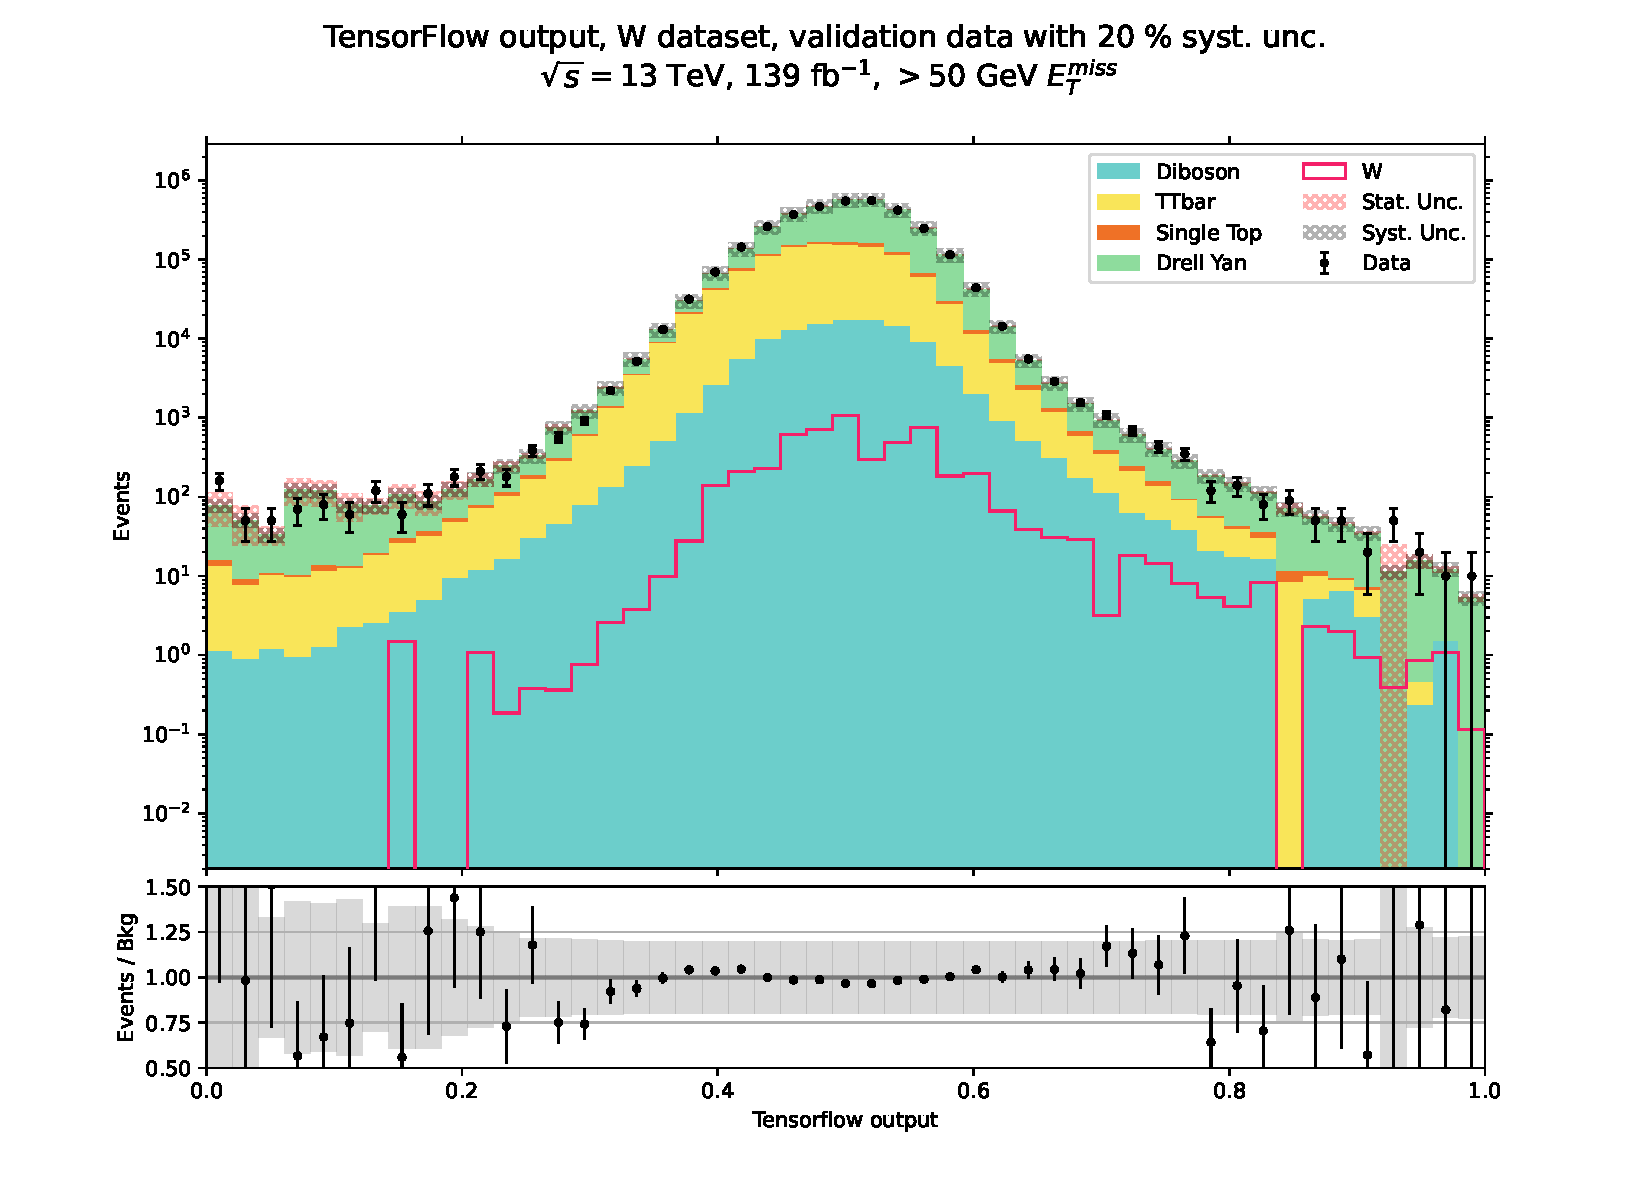
\includegraphics[width=1\textwidth]{bkg_MC/VAL.pdf}
        \caption{Weighing down bkg. wrt. $\frac{N_{sig,MC}}{N_{bkg,MC}}$ }
     \end{subfigure}
     \hfill
     \begin{subfigure}[b]{0.49\textwidth}
        \centering
        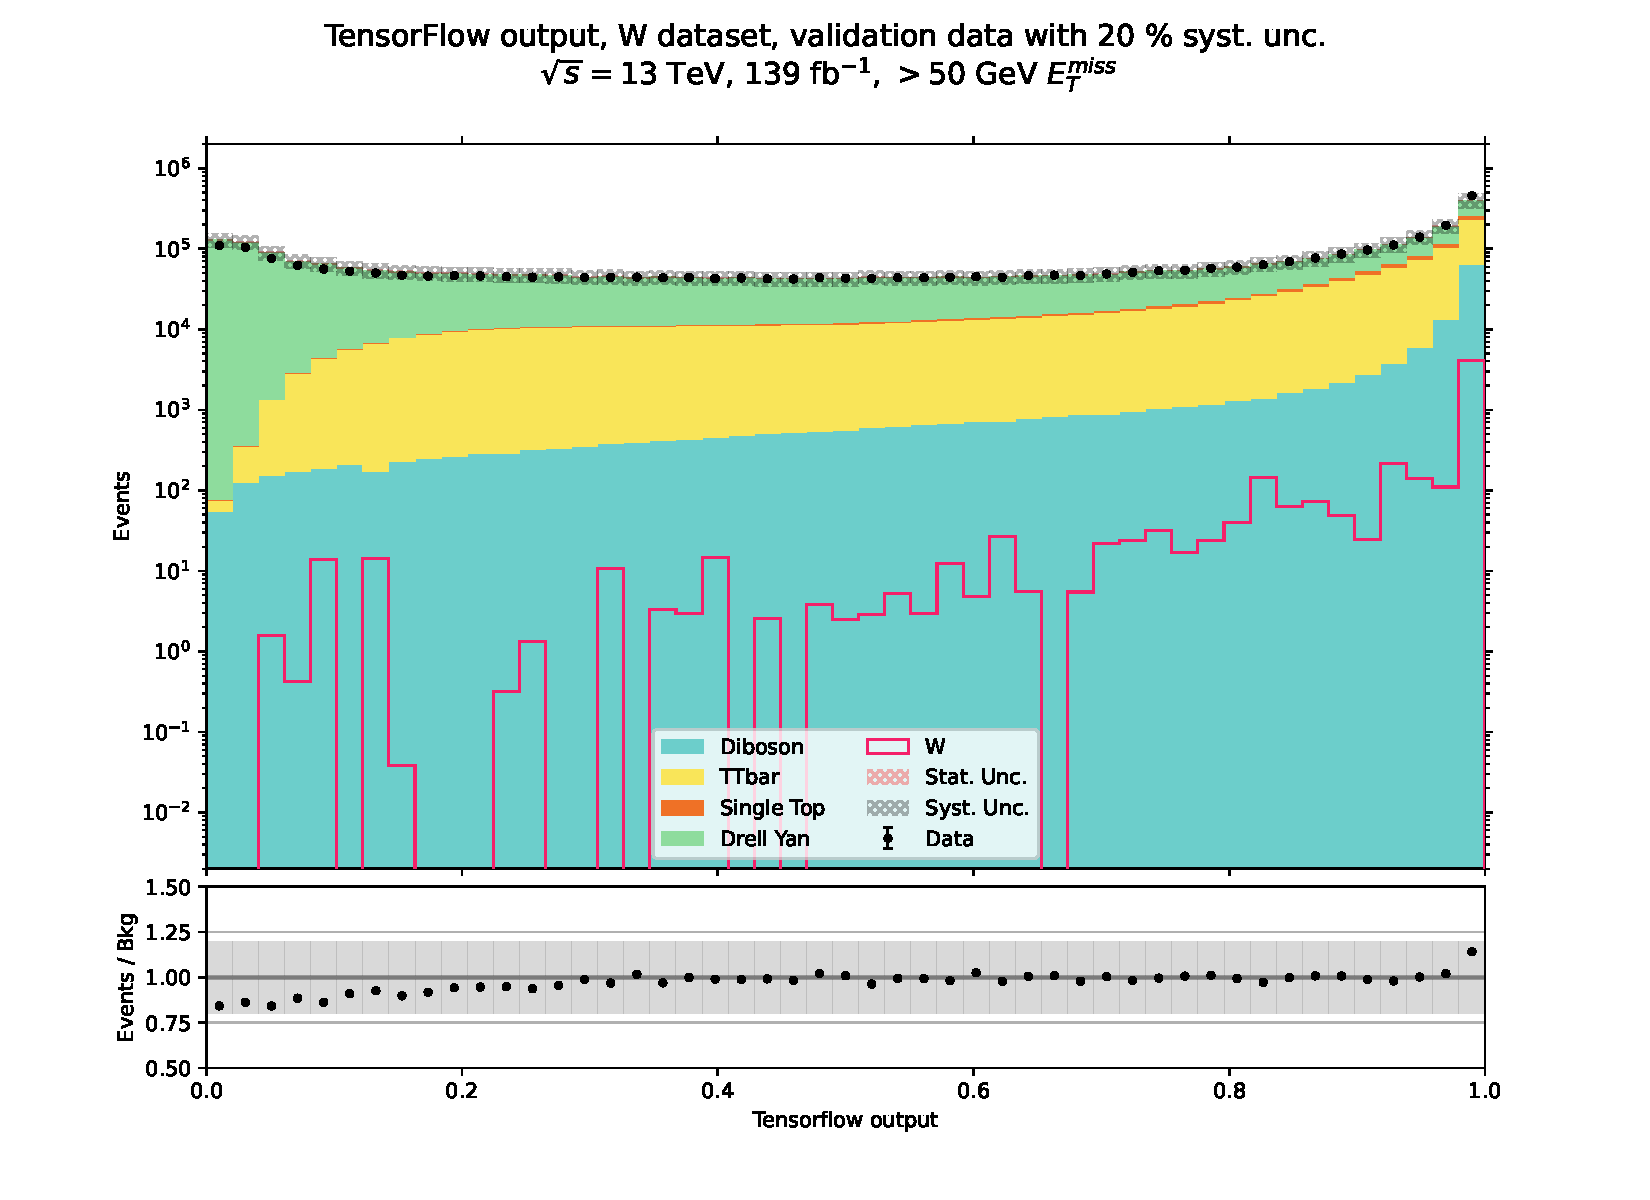
\includegraphics[width=1\textwidth]{sig_MC/VAL.pdf}
        \caption{Weighing up sig. wrt. $\frac{N_{bkg,MC}}{N_{sig,MC}}$}
     \end{subfigure}
     \hfill
     \begin{subfigure}[b]{0.49\textwidth}
          \centering
          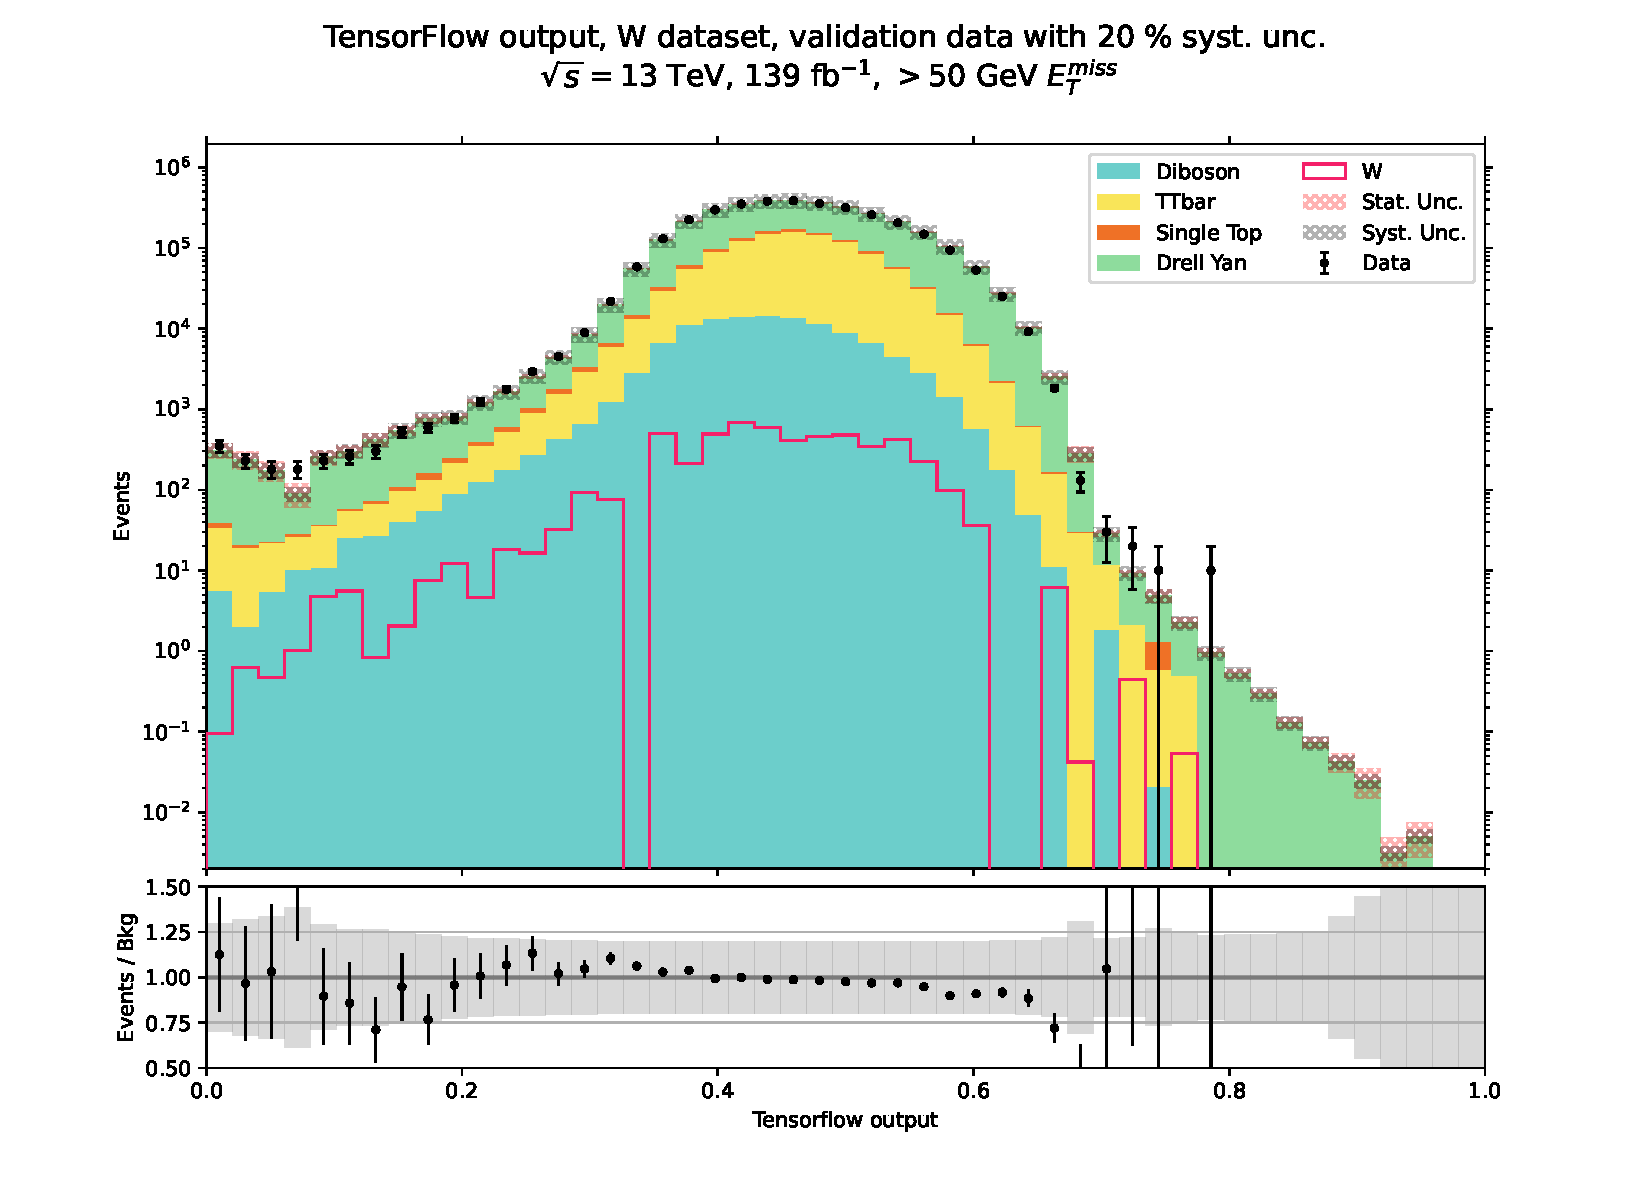
\includegraphics[width=1\textwidth]{bkg_exp/VAL.pdf}
          \caption{Weighing down bkg. wrt. $\frac{N_{sig,MC}}{N_{bkg,exp}}$ }
       \end{subfigure}
       \hfill
       \begin{subfigure}[b]{0.49\textwidth}
          \centering
          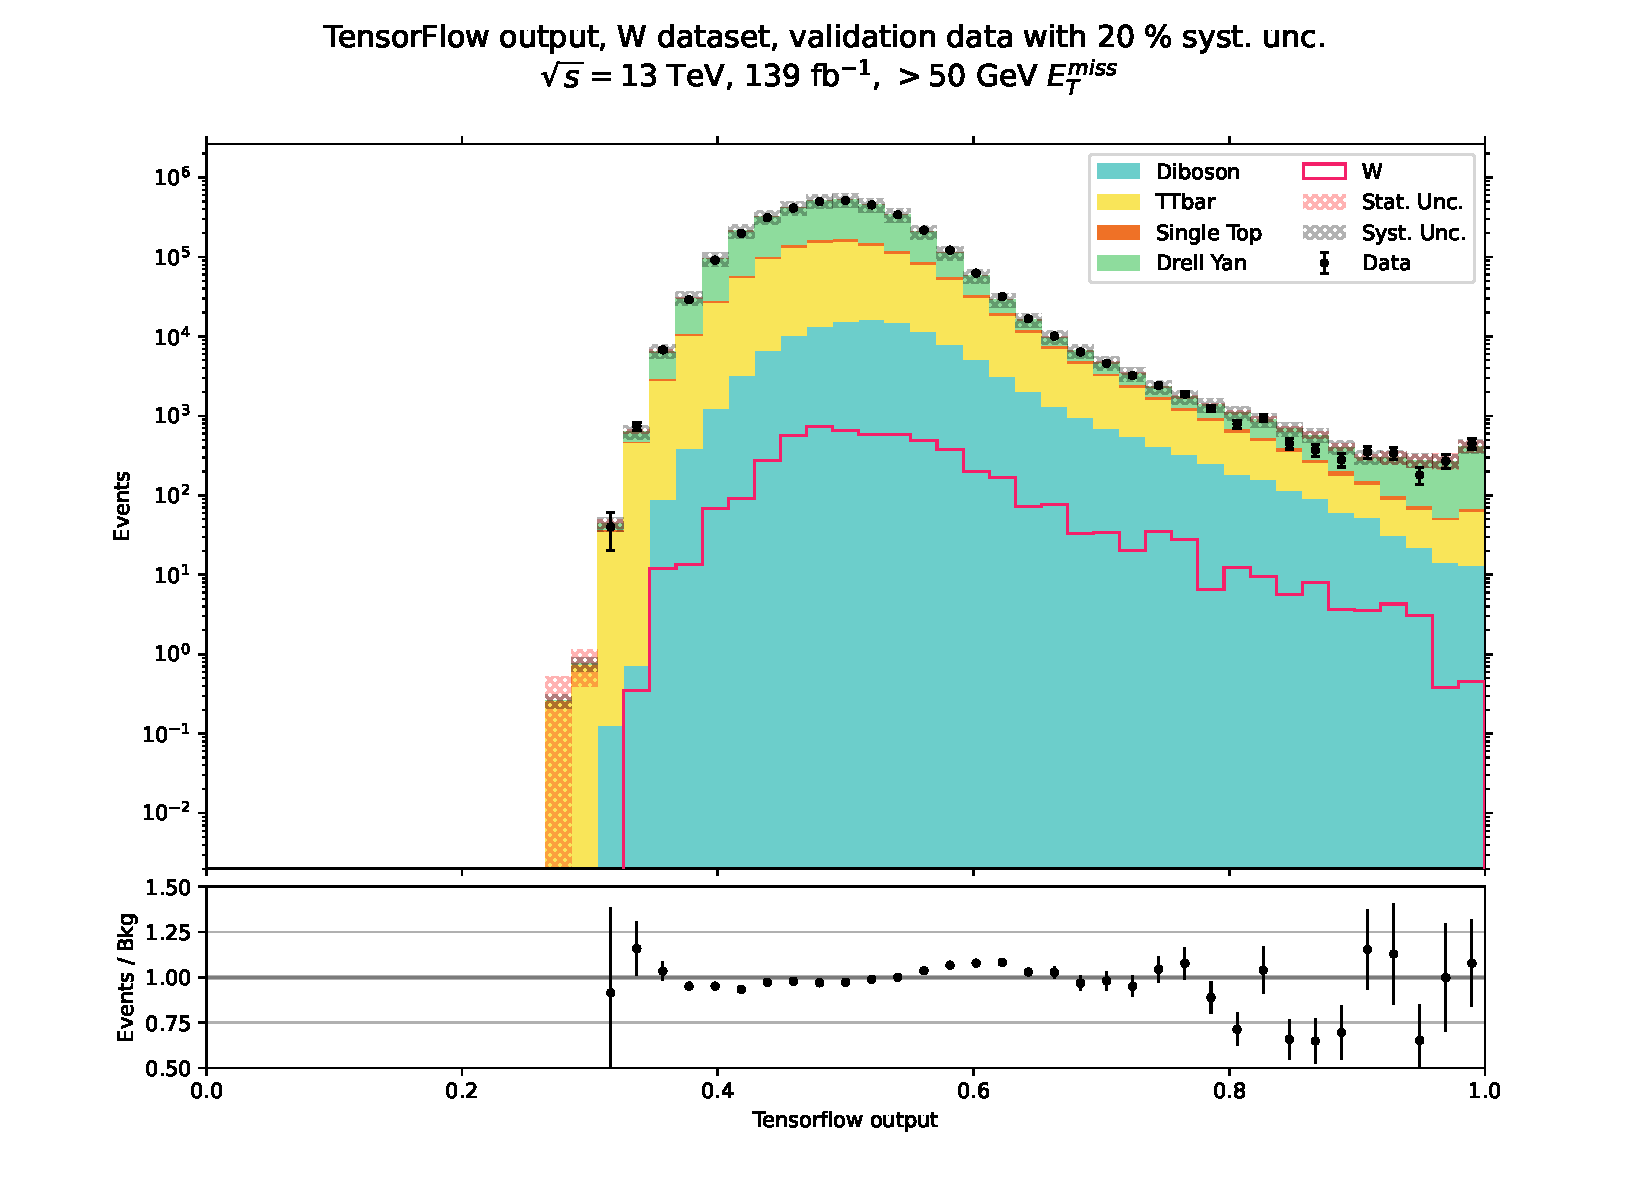
\includegraphics[width=1\textwidth]{sig_exp/VAL.pdf}
          \caption{Weighing up sig. wrt. $\frac{N_{bkg,exp}}{N_{sig,MC}}$}
       \end{subfigure}
     \caption[Validation plots for re-weighting background to expected events on NNs]{Validation plots of different balancing methods when re-weighting background events to expected events. 
     This was done using a dataset where the goal was to isolate the $W$ background process from other SM background processes} \label{fig:WVAL_rw}
\end{figure}
\clearpage
\begin{figure}[!ht]
	\centering
	\begin{subfigure}[b]{0.49\textwidth}
         \centering
         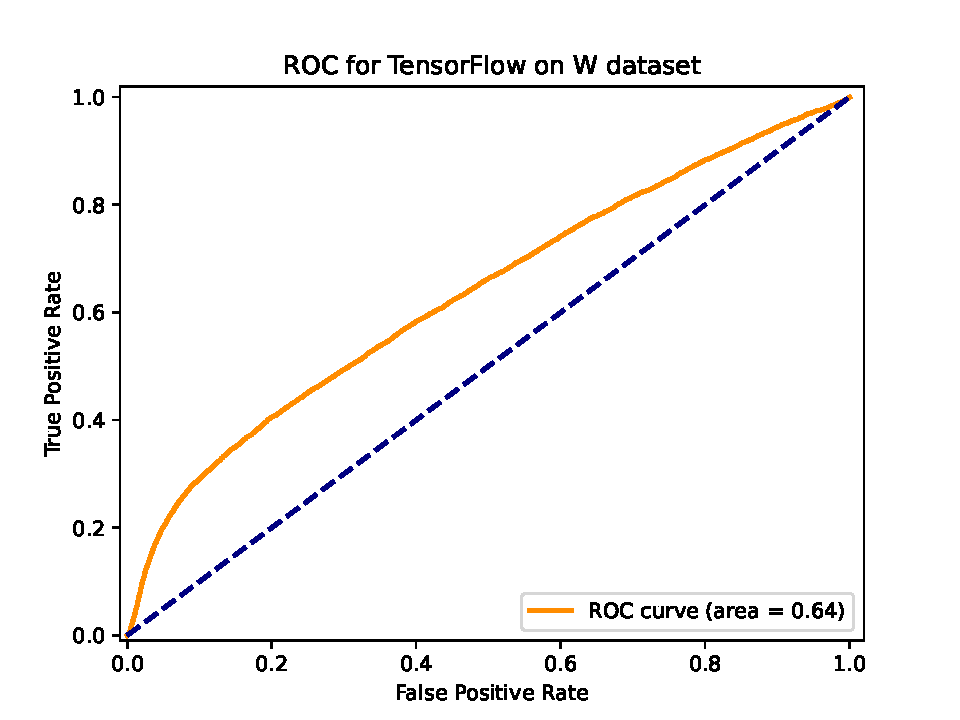
\includegraphics[width=1\textwidth]{bkg_MC/ROC.pdf}
         \caption{Weighing down bkg. wrt. $\frac{N_{sig,MC}}{N_{bkg,MC}}$ }
      \end{subfigure}
      \hfill
      \begin{subfigure}[b]{0.49\textwidth}
         \centering
         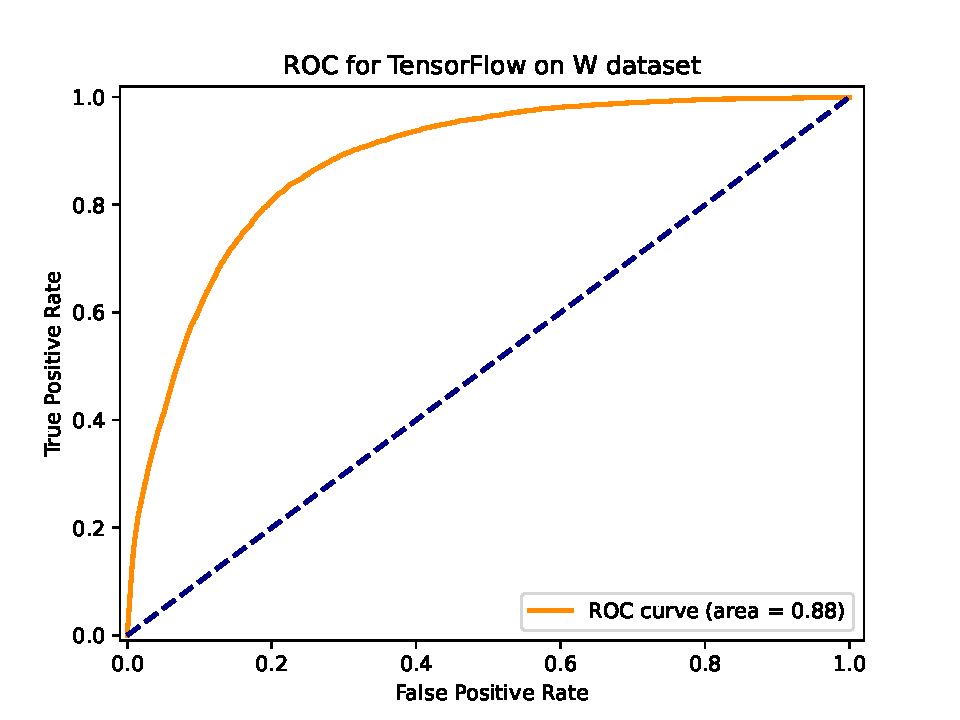
\includegraphics[width=1\textwidth]{sig_MC/ROC.pdf}
         \caption{Weighing up the signal wrt. $\frac{N_{bkg,MC}}{N_{sig,MC}}$}
      \end{subfigure}
      \hfill
      \begin{subfigure}[b]{0.49\textwidth}
            \centering
            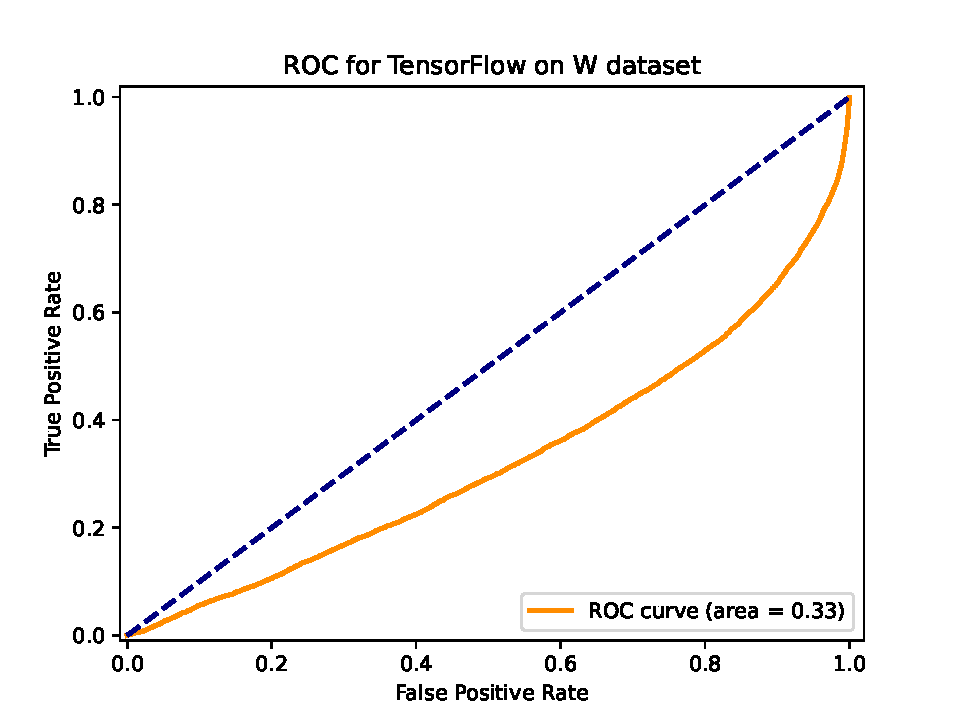
\includegraphics[width=1\textwidth]{bkg_exp/ROC.pdf}
            \caption{Weighing down bkg. wrt. $\frac{N_{sig,MC}}{N_{bkg,exp}}$ }
         \end{subfigure}
         \hfill
         \begin{subfigure}[b]{0.49\textwidth}
            \centering
            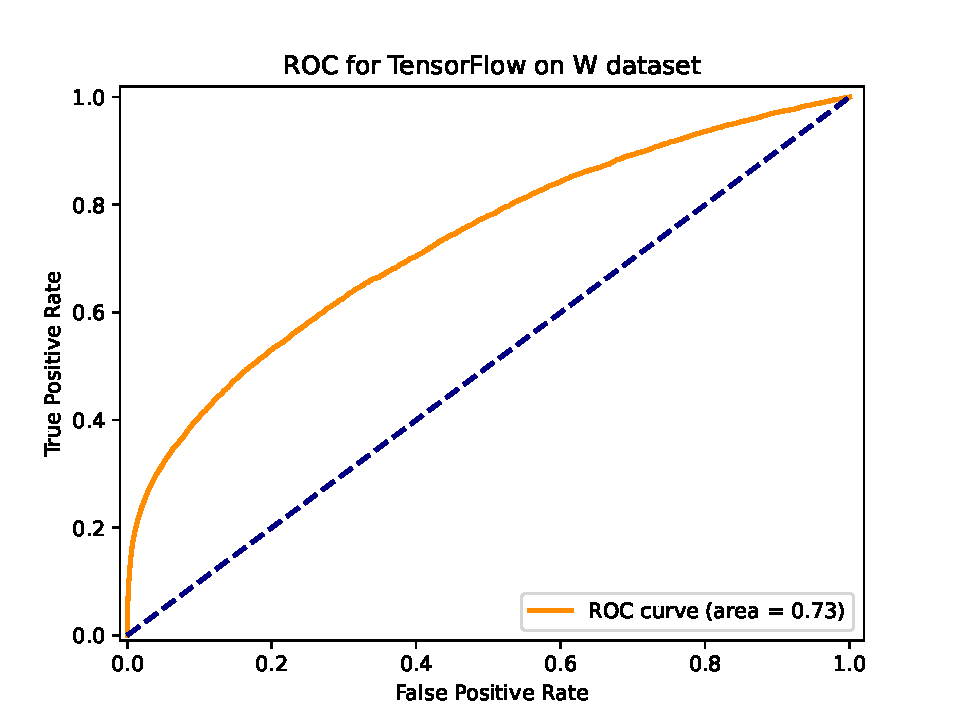
\includegraphics[width=1\textwidth]{sig_exp/ROC.pdf}
            \caption{Weighing up sig. wrt. $\frac{N_{bkg,exp}}{N_{sig,MC}}$}
         \end{subfigure}
      \caption[ROC plots for re-weighting background to expected events on NNs]{ROC plots of different balancing methods when re-weighting background events to expected events. 
      This was done using a dataset where the goal was to isolate the $W$ background process from other SM background processes}\label{fig:WROC_rw}
\end{figure}
\noindent As we are interested in having as high expected significance, we check whether the method of weighing down the background events, or the method of weighing up the signal events yields a higher expected significance. 
This is shown in Figure \ref{fig:WSIG}. Here we see that the expected significance is overall slightly higher when weighing up the signal events. Because of this we will continue our optimization search with this method \\
\begin{figure}[!ht]
	\centering
      \begin{subfigure}[b]{0.49\textwidth}
            \centering
            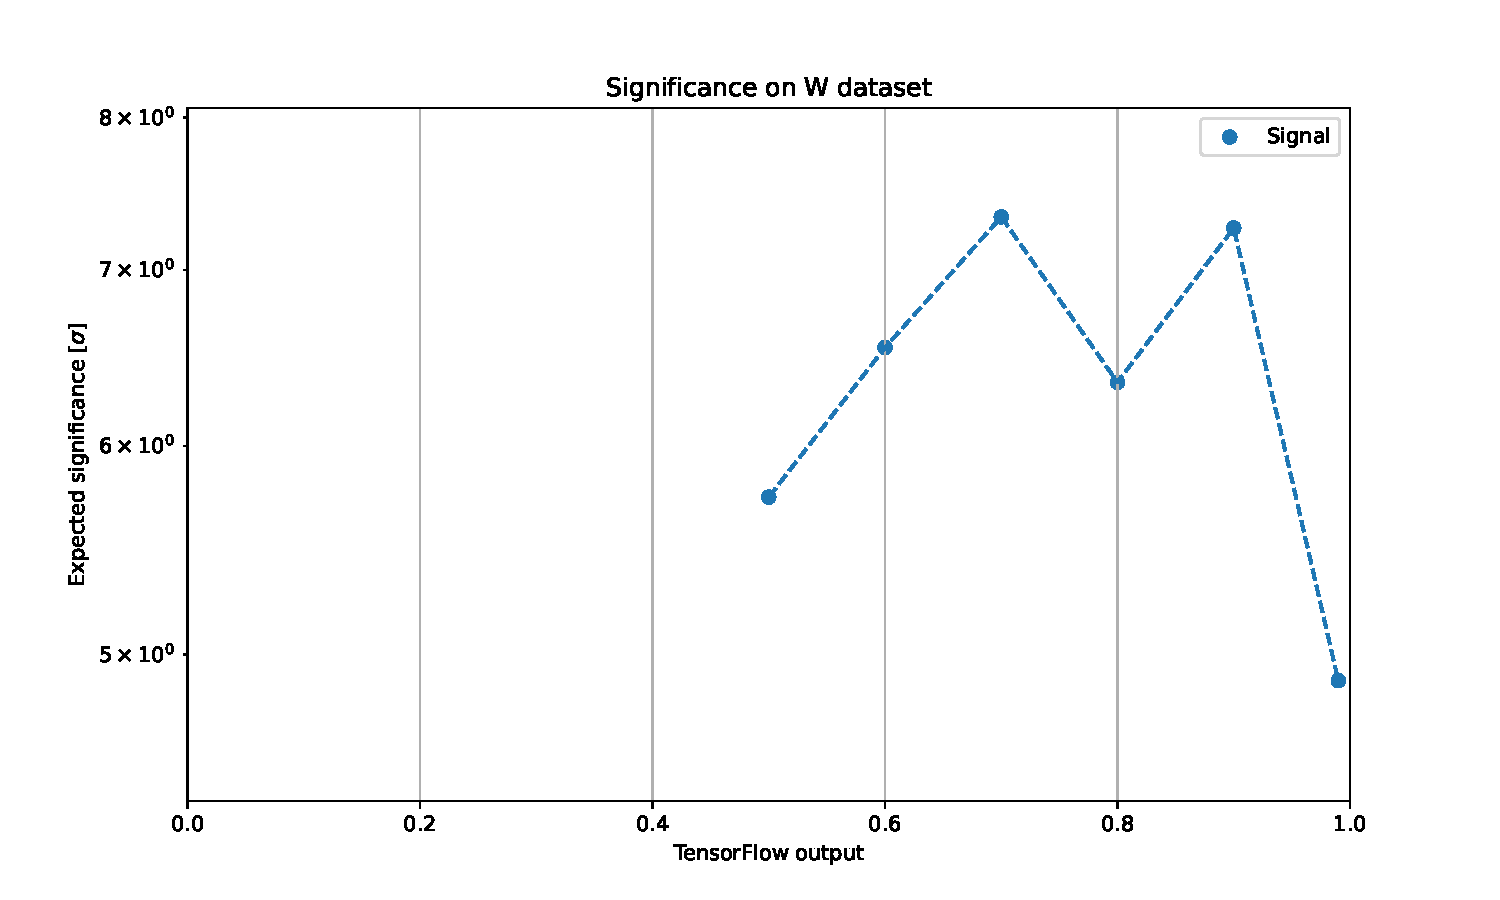
\includegraphics[width=1\textwidth]{bkg_exp/EXP_SIG.pdf}
            \caption{Weighing down bkg. wrt. $\frac{N_{sig,MC}}{N_{bkg,exp}}$ }
         \end{subfigure}
         \hfill
         \begin{subfigure}[b]{0.49\textwidth}
            \centering
            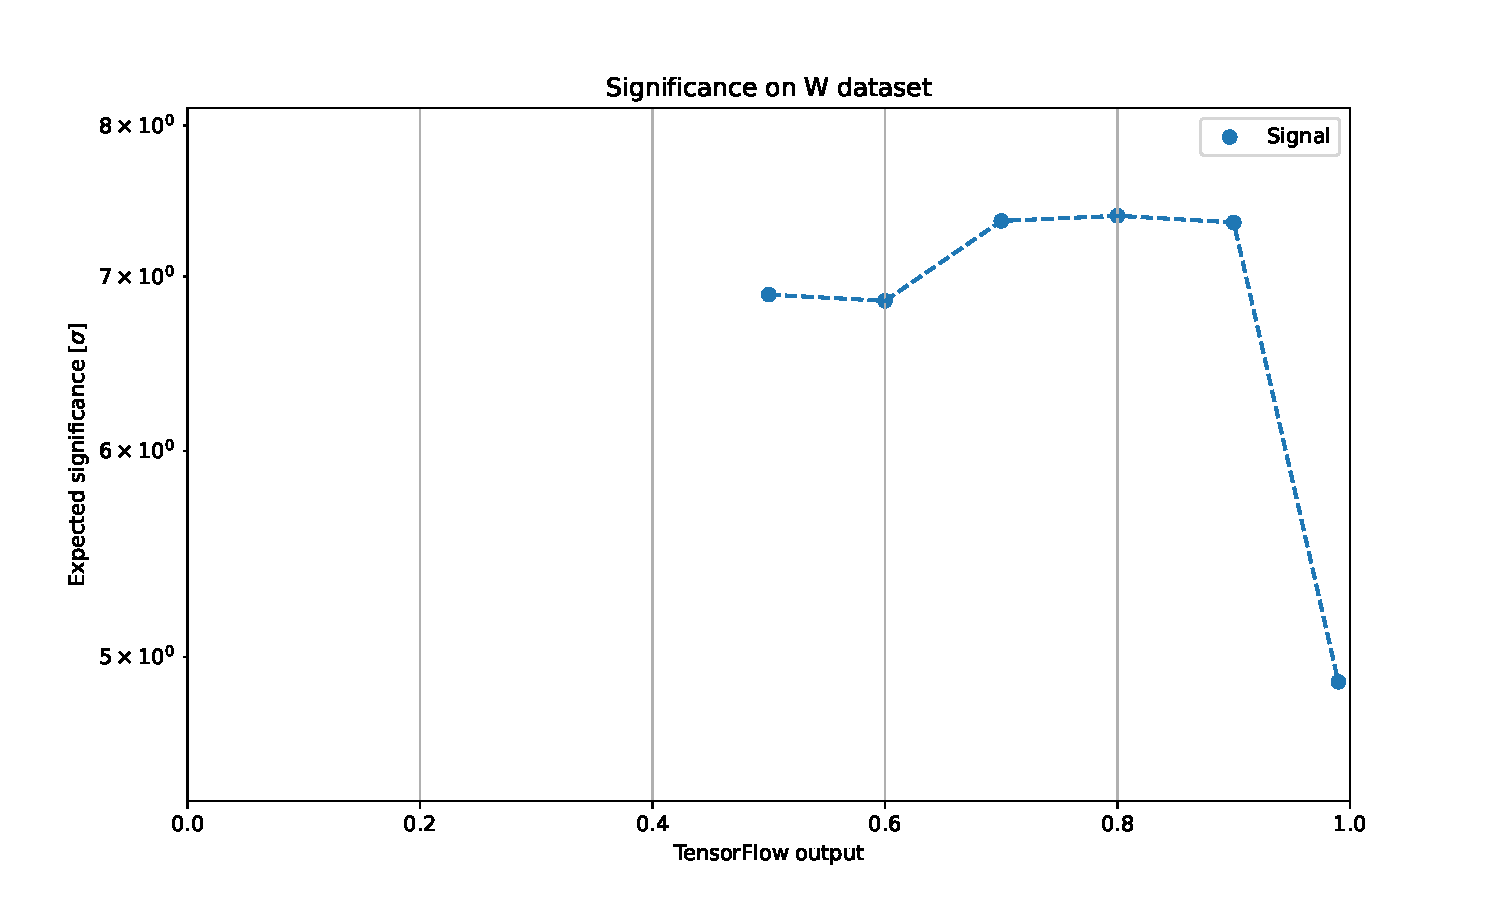
\includegraphics[width=1\textwidth]{sig_exp/EXP_SIG.pdf}
            \caption{Weighing up sig. wrt. $\frac{N_{bkg,exp}}{N_{sig,MC}}$}
         \end{subfigure}
      \caption[Significance plots for re-weighting and balancing W dataset on NNs]{Expected significance plots of the best balancing methods when re-weighting background events to expected events. 
      This was done using a dataset where the goal was to isolate the $W$ background process from other SM background processes}\label{fig:WSIG}
\end{figure}
\\As a last note for the testing of these methods, the networks do not have the best distribution on the validation plots. The reason for this might be because 
we did not optimize the networks we tested, but rather used the same network for test. For the next test, which is of the padding of the variables we will conduct a grid search to find the best hyperparameters.
\clearpage


\subsection{Padding of data}\label{sec:padding_NN_res}
For the padding problem. We will as explained in Chapter \ref{sec:padding_NN} try the new variables presented in Table \ref{tab:padding_variables}. The other method we tried was to remove the features with jagged arrays, that means the $p_T, \eta, \phi$ of the three most energetic jets, as well as the invariant mass of the two most energetic ones, $m_{jj}$.
The trained a network using 80\% of the whole SM background events as well as 80\% of all the Z' DH HDS samples. As sample weights we used the best method from the previous section, which was to re-weight every background event and balance the dataset by weighing up all signal events by the ratio of expected number of background events over signal MC events, $\frac{N_{bkg,exp}}{N_{sig,MC}}$. 
As the best normalization method was \verb|Batch_normalization|, this method was used here. We also utilized the ADAM optimizer instead of SGD.\\
\\As changing features changes the whole dataset, then to get the best results as possible we went through a full grid search following the steps in Chapter \ref{sec:NNgriddy} for both networks. The result for the hyperparameters that gave the highest significance can be seen in Figure \ref{fig:pad_griddy}.
\graphicspath{{../../Plots/NeuralNetwork/Padding/}}
\begin{figure}[!ht]
	\centering
	\begin{subfigure}[b]{0.49\textwidth}
      \centering
      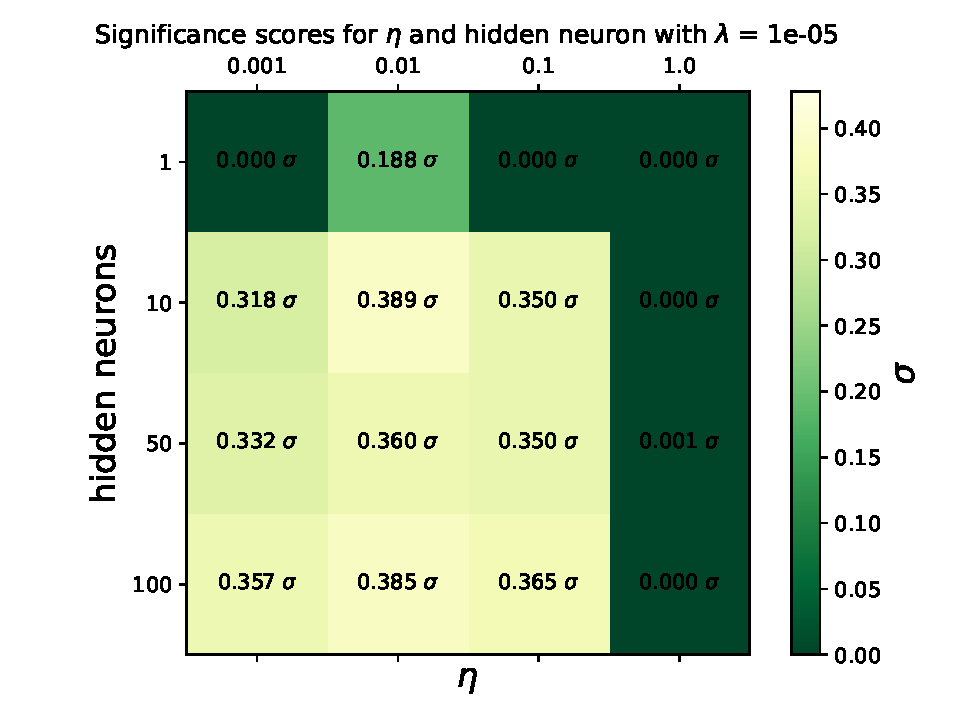
\includegraphics[width=1\textwidth]{New_pad/GRID/Significance_ne.pdf}
      % \includegraphics[width=1\textwidth]{New_pad/GRID/AUC/Testing_nl.pdf}
      \caption{When including new features}
   \end{subfigure}
   \hfill
	\begin{subfigure}[b]{0.49\textwidth}
      \centering
      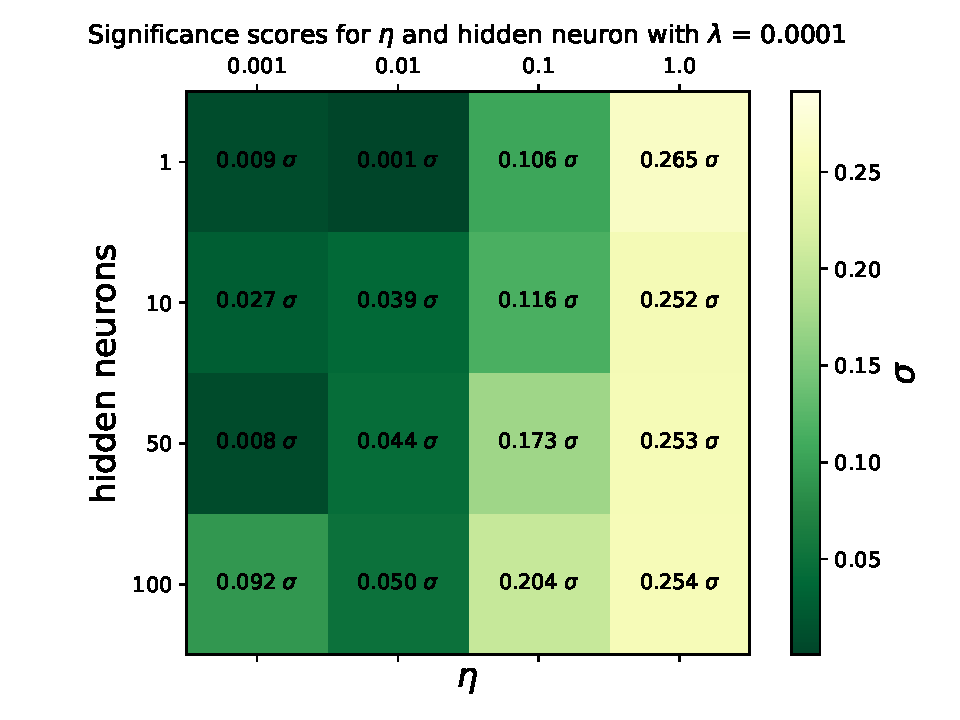
\includegraphics[width=1\textwidth]{No_pad/GRID/Significance_ne.pdf}
      % \includegraphics[width=1\textwidth]{No_pad/GRID/AUC/Testing_nl.pdf}
      \caption{When dropping features}
   \end{subfigure}
   \caption[Grid search result for pad testing on NN]{Grid search result for pad testing on NN.  This is training a dataset with 80\% of all Z' DH HDS events.}\label{fig:pad_griddy}
\end{figure}
\\This means that the best hyperparameters for both networks coincidentally is the same, meaning: \verb|n_neuron = 10,| \verb|eta = 0.01,| \verb|lamda = 1e-5|. The loss, AUC and binary accuracy over epochs for the best networks can be seen in Figure \ref{fig:NN_stats_pad} and Figure \ref{fig:NN_stats_no_pad}.
\begin{figure}[!ht]
	\centering
	\begin{subfigure}[b]{0.49\textwidth}
      \centering
      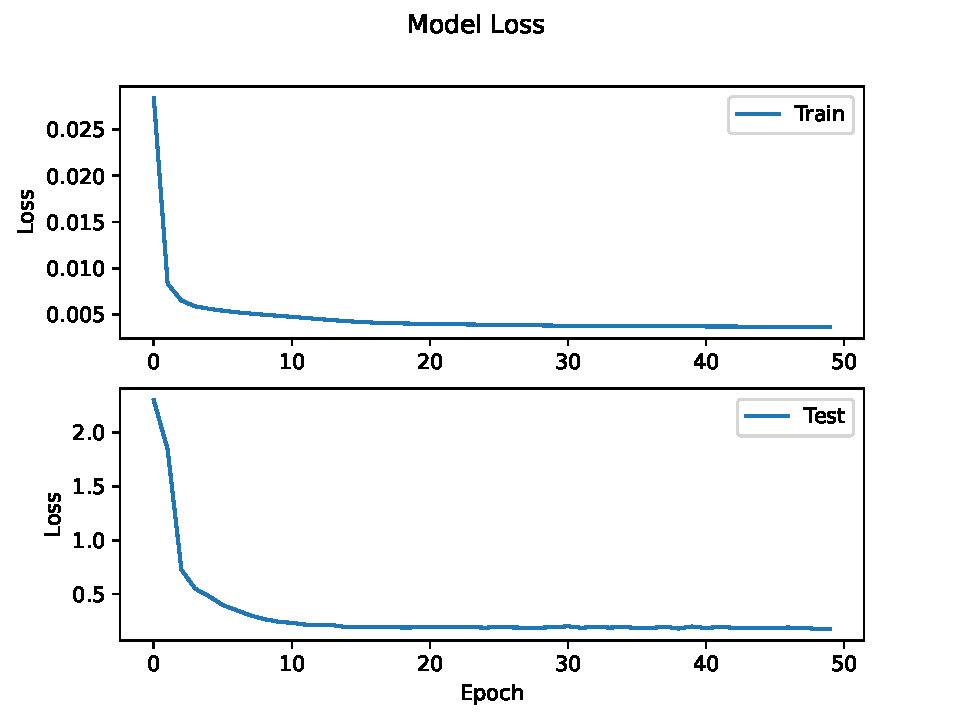
\includegraphics[width=1\textwidth]{New_pad/Loss.pdf}
   \end{subfigure}
   \hfill
	\begin{subfigure}[b]{0.49\textwidth}
      \centering
      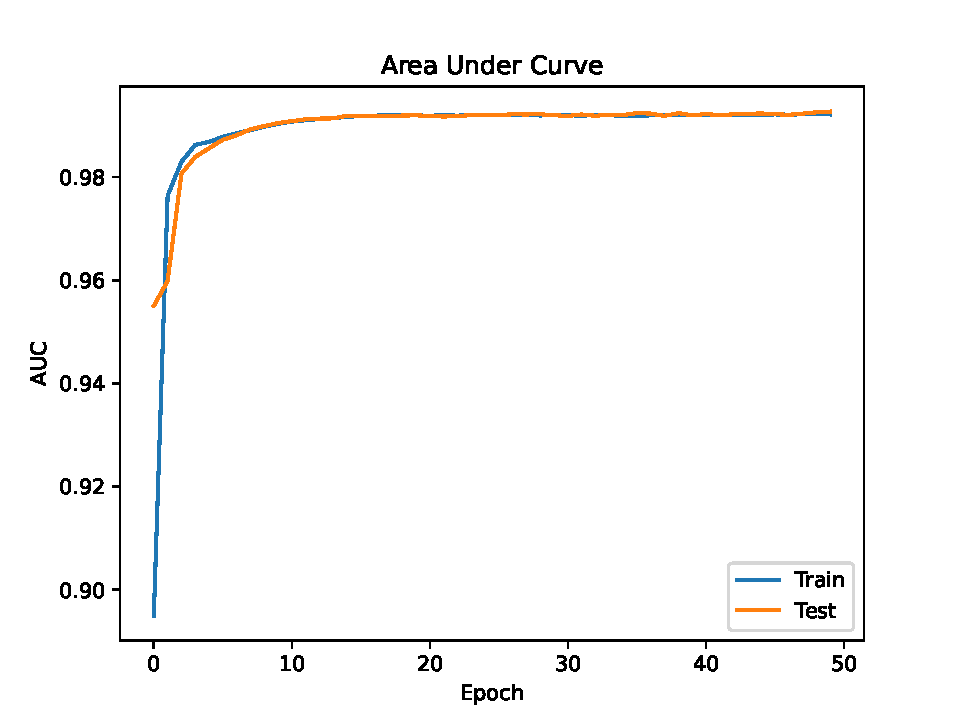
\includegraphics[width=1\textwidth]{New_pad/AUC.pdf}
   \end{subfigure}
   \hfill
	\begin{subfigure}[b]{0.49\textwidth}
      \centering
      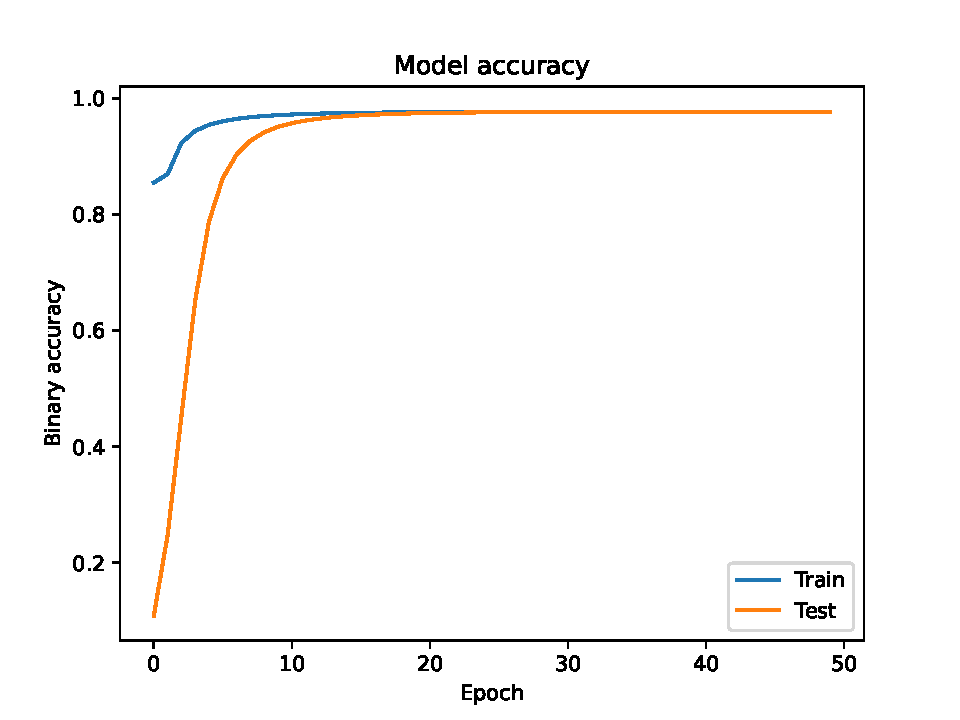
\includegraphics[width=1\textwidth]{New_pad/Binary_accuracy.pdf}
   \end{subfigure}
   \caption[NN parameters after 50 epochs with new features]{NN parameters after 50 epochs with new features.  This is training a dataset with 80\% of all Z' DH HDS events.}\label{fig:NN_stats_pad}
\end{figure}
\begin{figure}[!ht]
	\centering
	\begin{subfigure}[b]{0.49\textwidth}
      \centering
      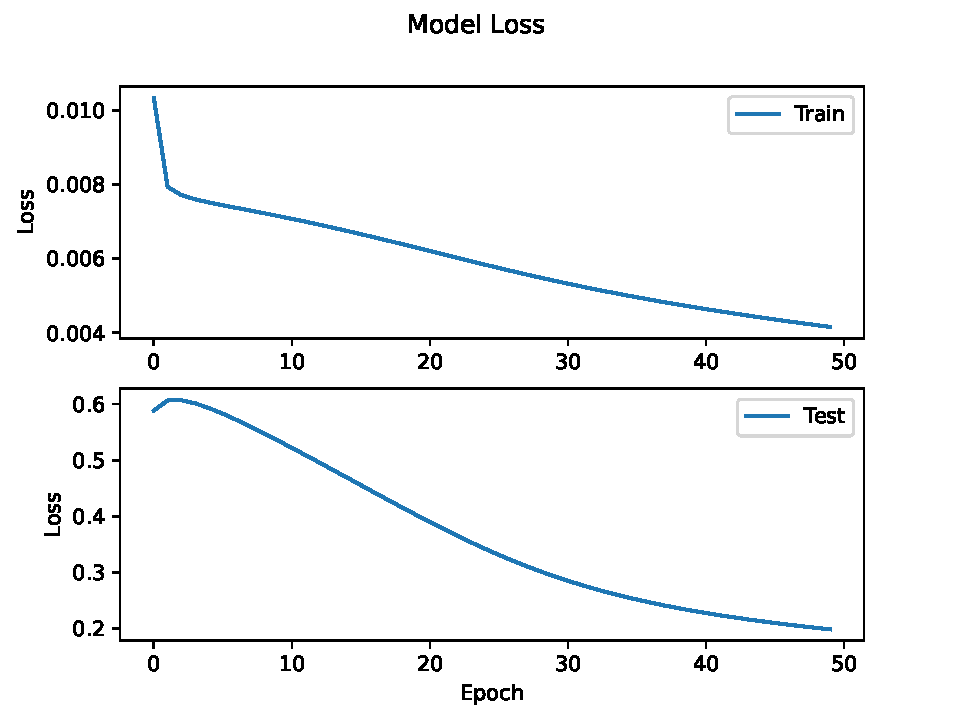
\includegraphics[width=1\textwidth]{No_pad/Loss.pdf}
   \end{subfigure}
   \hfill
	\begin{subfigure}[b]{0.49\textwidth}
      \centering
      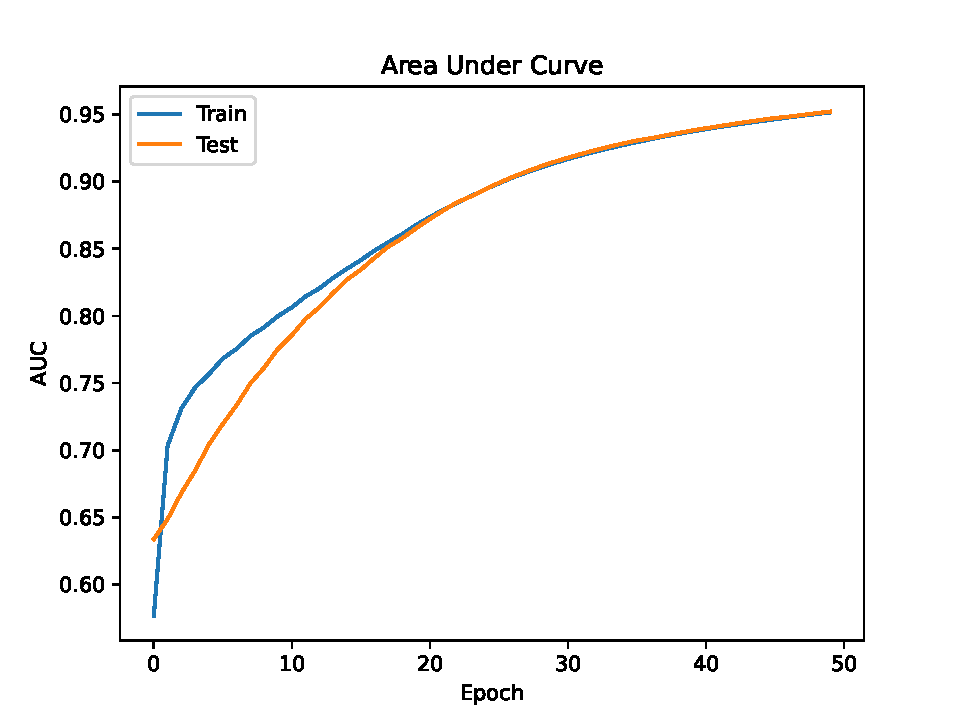
\includegraphics[width=1\textwidth]{No_pad/AUC.pdf}
   \end{subfigure}
   \hfill
	\begin{subfigure}[b]{0.49\textwidth}
      \centering
      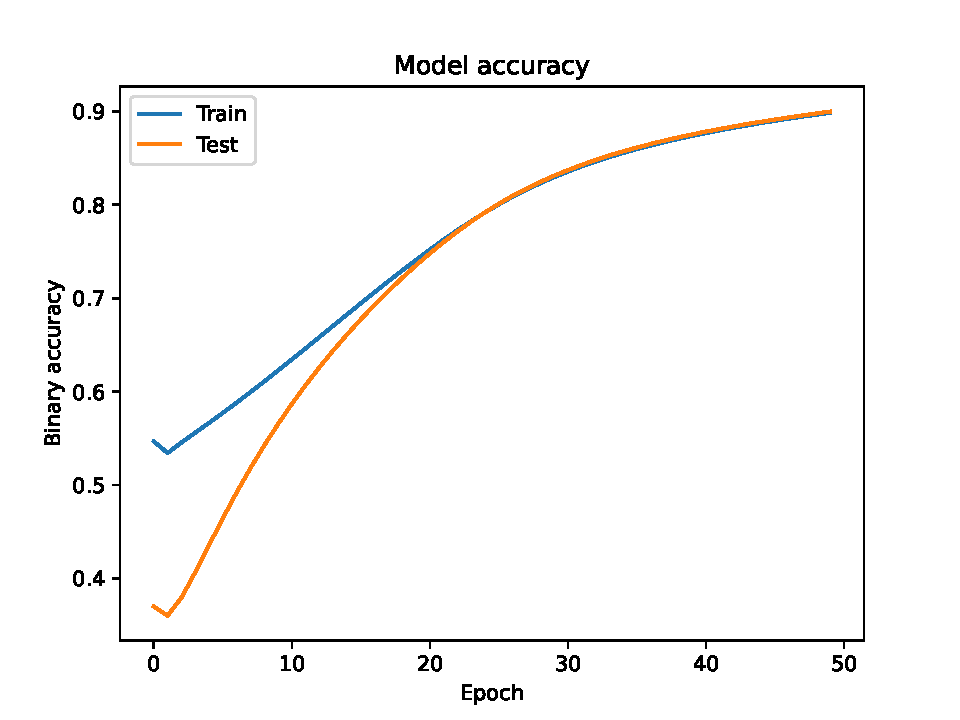
\includegraphics[width=1\textwidth]{No_pad/Binary_accuracy.pdf}
   \end{subfigure}
   \caption[NN parameters after 50 epochs when dropping features]{NN parameters after 50 epochs when dropping features.  This is training a dataset with 80\% of all Z' DH HDS events.}\label{fig:NN_stats_no_pad}
\end{figure}
\clearpage\noindent We tested on the remaining 20\% of the SM background events, as well as 20\% of Z' DH HDS events where $m_{Z'} =130$ GeV. The ROC scores for each network can be seen in Figure \ref{fig:NN_pad_ROC}. The validation plots can be seen in Figure \ref{fig:NN_pad_VAL}
\begin{figure}[!ht]
	\centering
	\begin{subfigure}[b]{0.49\textwidth}
      \centering
      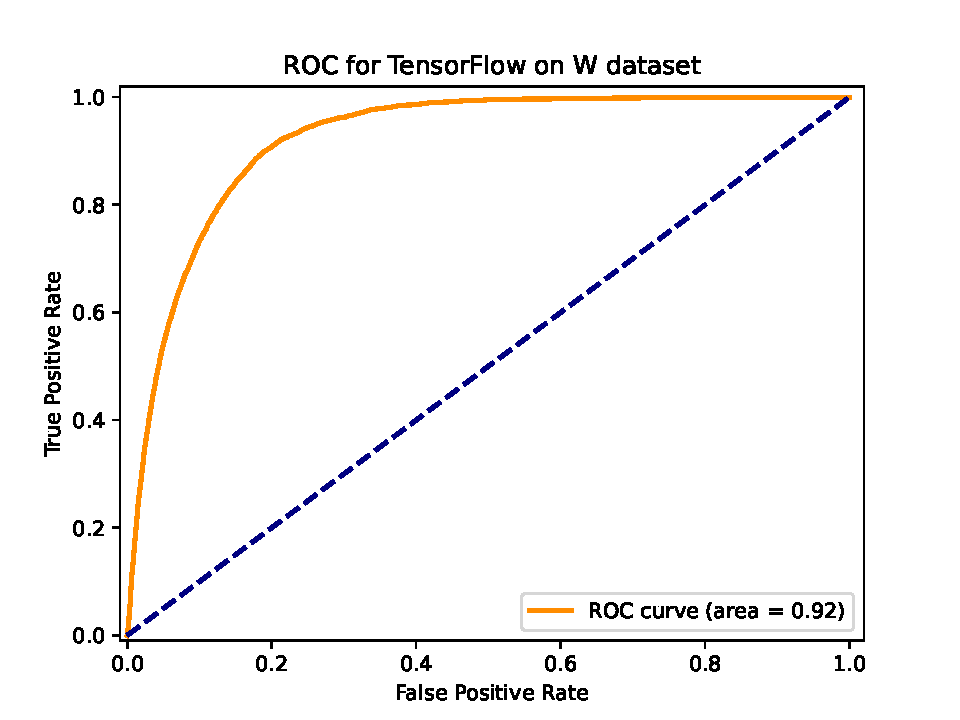
\includegraphics[width=1\textwidth]{New_pad/ROC.pdf}
      \caption{When including new features}
   \end{subfigure}
   \hfill
	\begin{subfigure}[b]{0.49\textwidth}
      \centering
      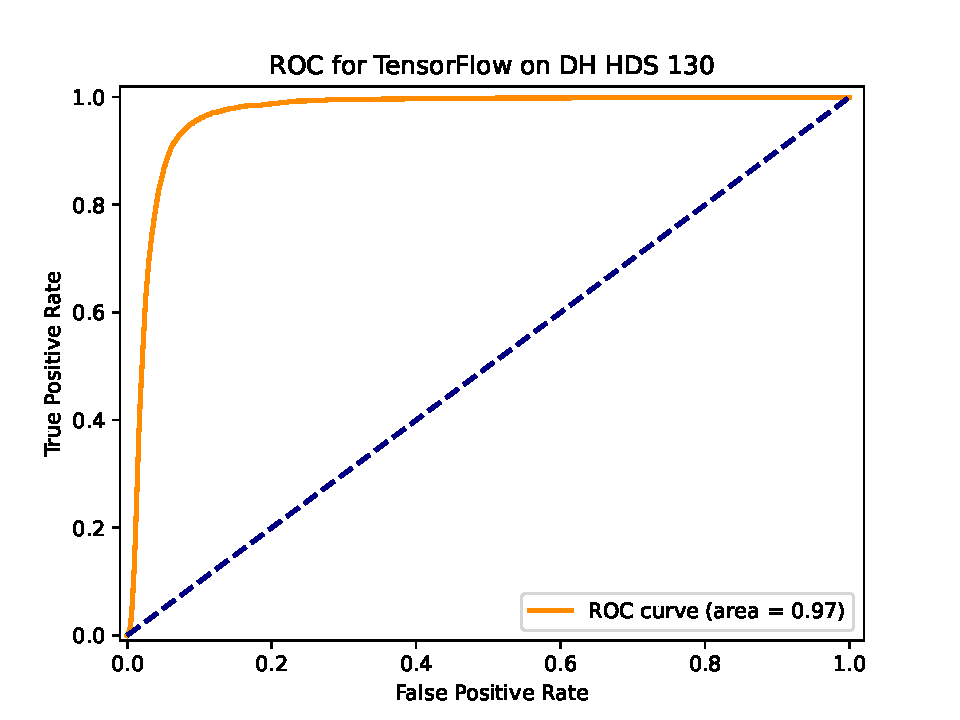
\includegraphics[width=1\textwidth]{No_pad/ROC.pdf}
      \caption{When dropping features}
   \end{subfigure}
   \caption[ROC plots for both padding methods]{ROC plots for both padding methods.  This is testing a dataset with 20\% of the Z' DH HDS $m_{Z'}=130$ GeV events.}\label{fig:NN_pad_ROC}
\end{figure}
\begin{figure}[!ht]
	\centering
	\begin{subfigure}[b]{0.49\textwidth}
      \centering
      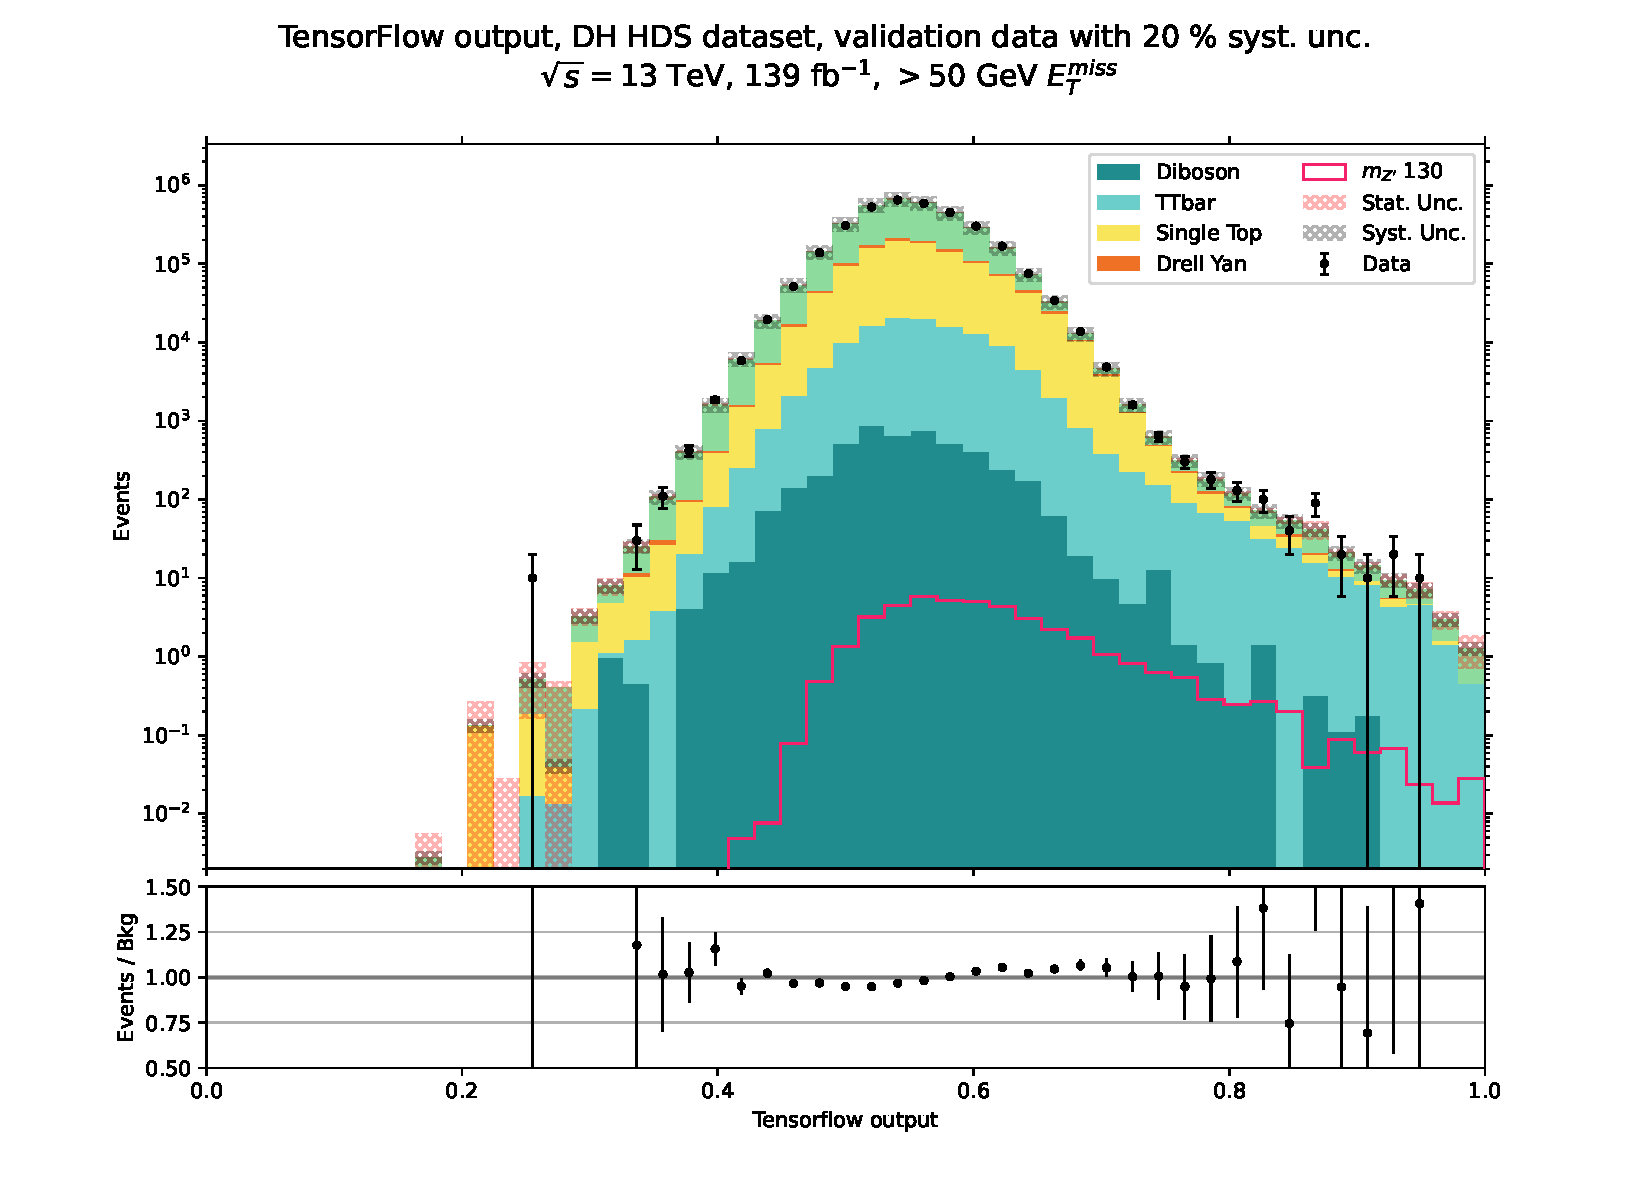
\includegraphics[width=1\textwidth]{New_pad/VAL.pdf}
      \caption{When including new features}
   \end{subfigure}
   \hfill
	\begin{subfigure}[b]{0.49\textwidth}
      \centering
      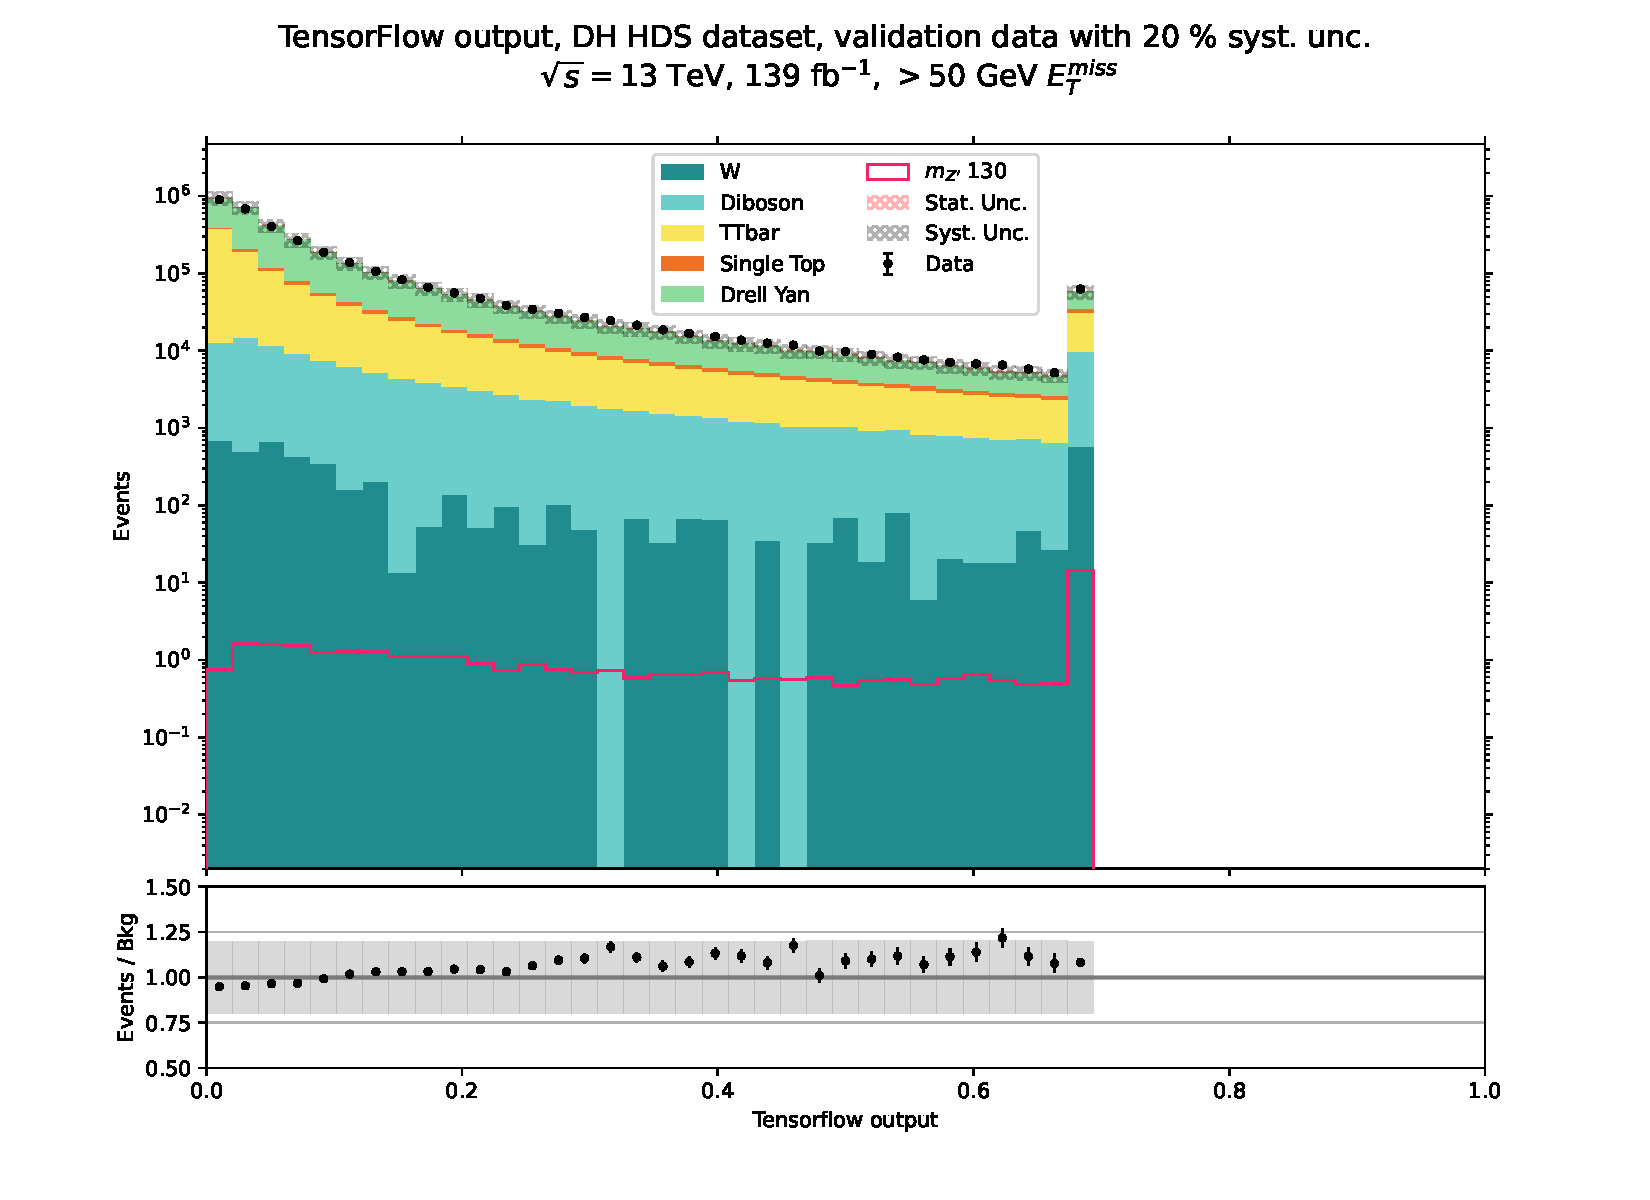
\includegraphics[width=1\textwidth]{No_pad/VAL.pdf}
      \caption{When dropping features}
   \end{subfigure}
   \caption[Validation plots for both padding methods]{Validation plots for both padding methods.  This is testing a dataset with 20\% of the Z' DH HDS $m_{Z'}=130$ GeV events.}\label{fig:NN_pad_VAL}
\end{figure}
\\As we can see the performance of both methods is the same, to check if the sensitivity increases more with the new padding method or not we can check the significance of each model. This can be seen in Figure \ref{fig:NN_pad_SIG}, which shows a slight improvement on the sensitivity of the network when using the features.
\begin{figure}[!ht]
	\centering
	\begin{subfigure}[b]{0.49\textwidth}
      \centering
      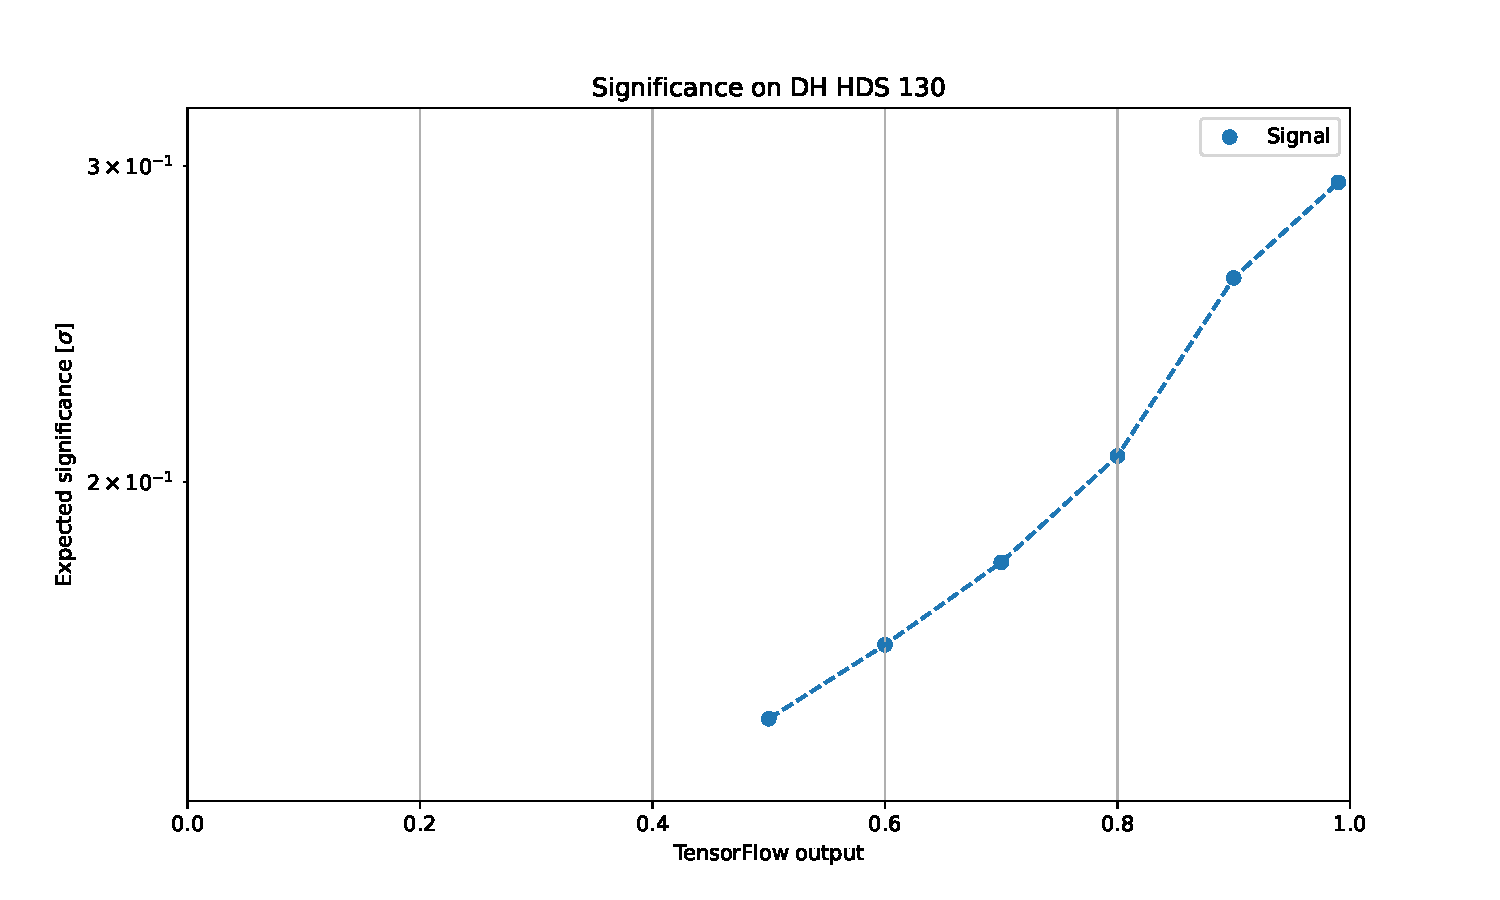
\includegraphics[width=1\textwidth]{New_pad/EXP_SIG.pdf}
      \caption{When including new features}
   \end{subfigure}
   \hfill
	\begin{subfigure}[b]{0.49\textwidth}
      \centering
      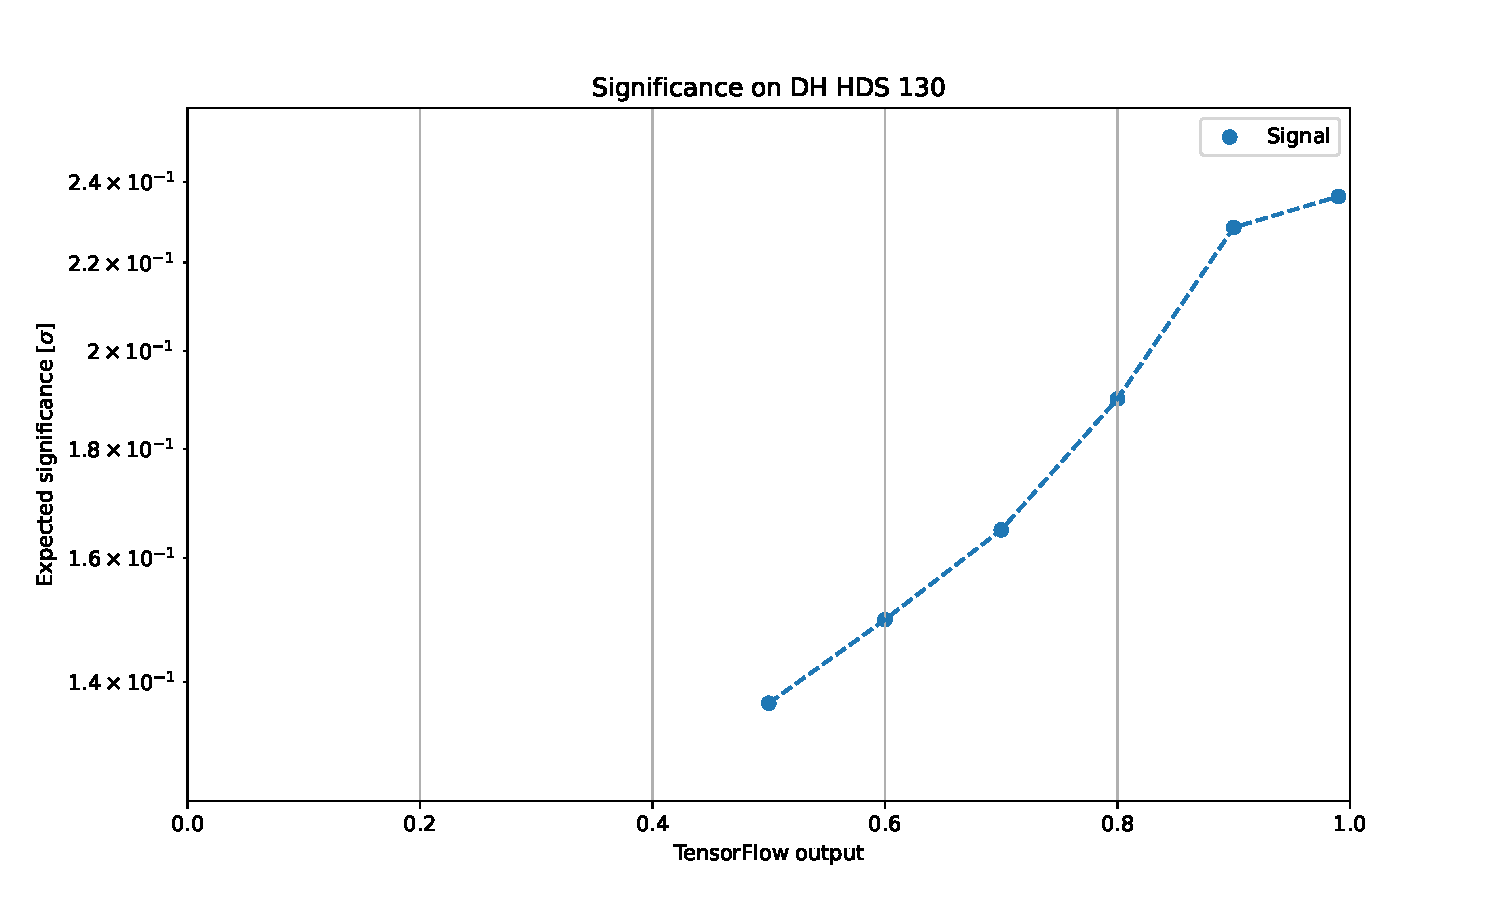
\includegraphics[width=1\textwidth]{No_pad/EXP_SIG.pdf}
      \caption{When dropping features}
   \end{subfigure}
   \caption[Significance plots for both padding methods]{Significance plots for both padding methods.  This is testing a dataset with 20\% of the Z' DH HDS $m_{Z'}=130$ GeV events.}\label{fig:NN_pad_SIG}
\end{figure}
\clearpage




\section{Boosted Decision Tree Training}
As the only technique that needed to be tested for BDTs was the different weighting methods, we conducted these here. We only tested the weighting techniques where we only look at the positive weights, and where we scale the weights 
wrt. the sum of the weights over the sum over the absolute value of weights. To compare we also included the unweighted method (only balancing data). The hyperparameters used to train the different networks in this chapter were
\begin{itemize}
   \item L2-$\lambda$ = 10$^{-5}$
   \item Number of trees = 200
   \item Depth of trees = 6
   \item Learning rate $\eta$ = 0.1
\end{itemize}
\clearpage
\subsection{Weights}
The results of the different weighting methods can be seen in Figure \ref{fig:BDT_wgts}.\\
\graphicspath{{../../Plots/XGBoost/Weighting_methods/}}
\begin{figure}[!ht]
	\centering
	\begin{subfigure}[b]{0.49\textwidth}
      \centering
      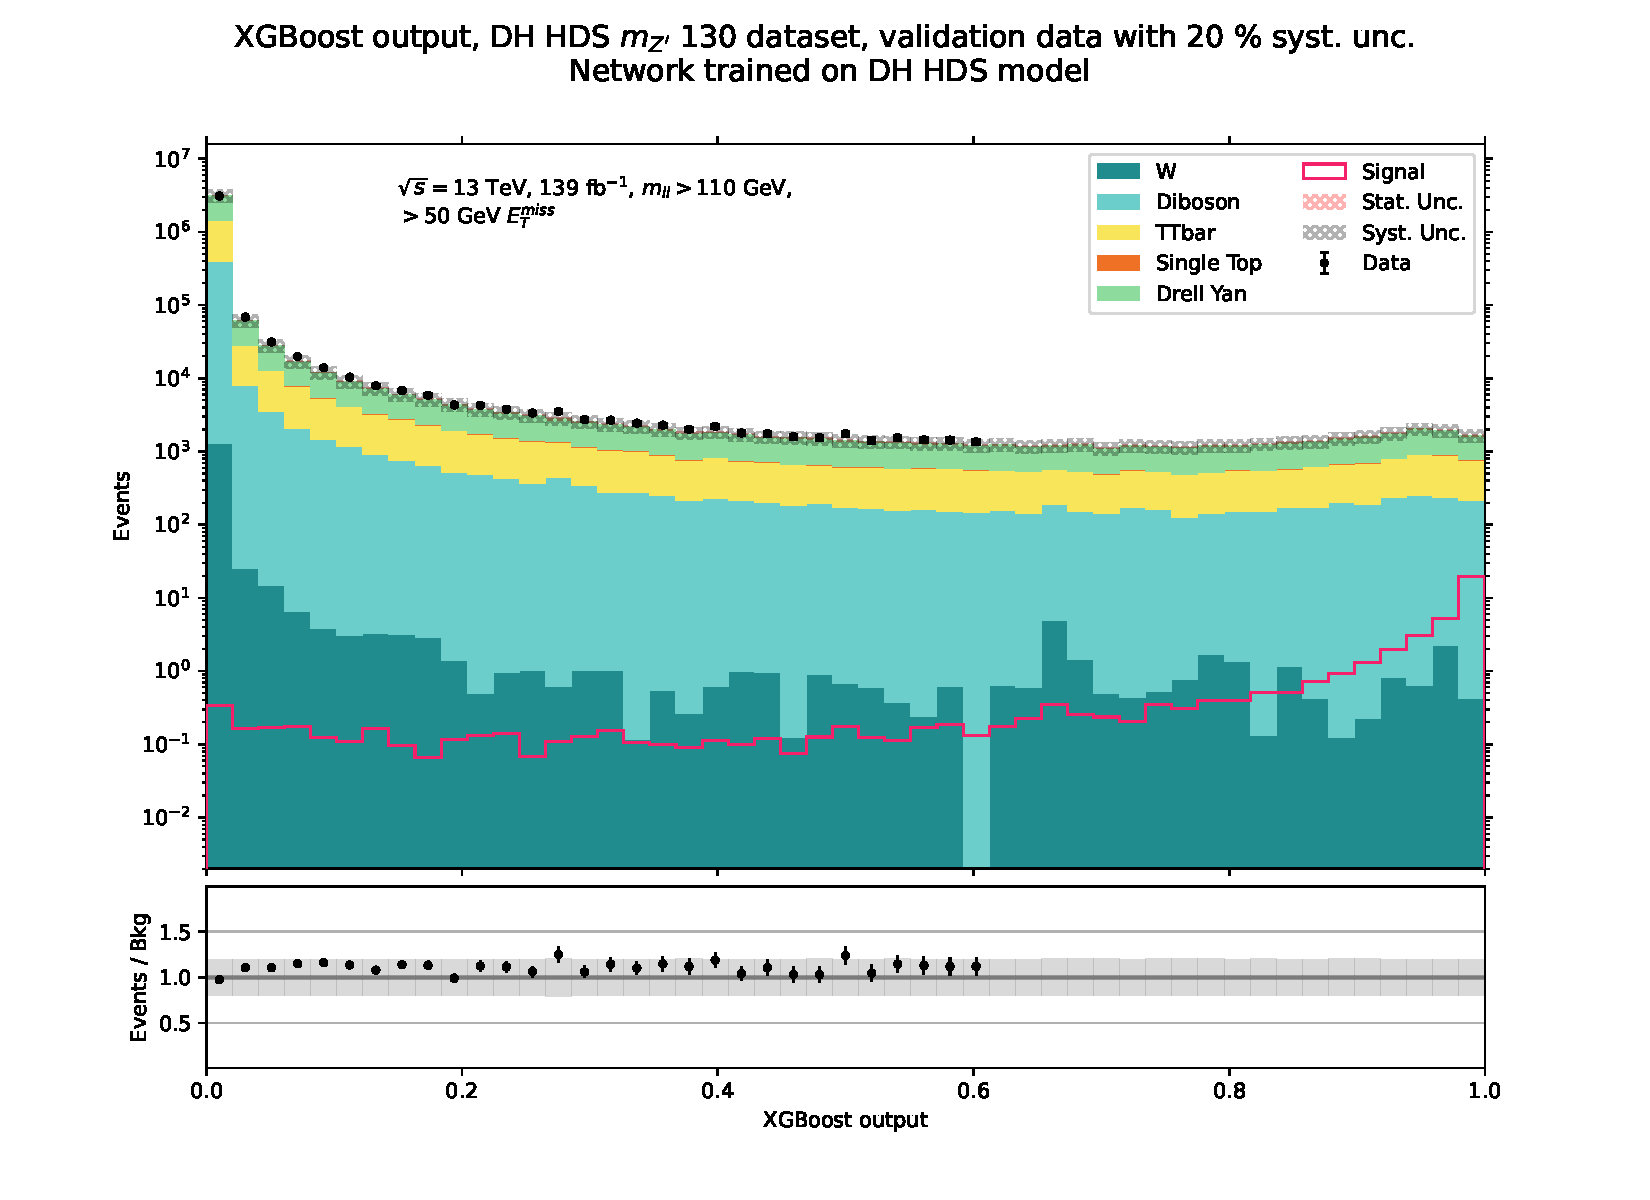
\includegraphics[width=1\textwidth]{Abs_wgt/VAL.pdf}
      \caption{Using scaled absolute value of weights}
   \end{subfigure}
   \begin{subfigure}[b]{0.49\textwidth}
      \centering
      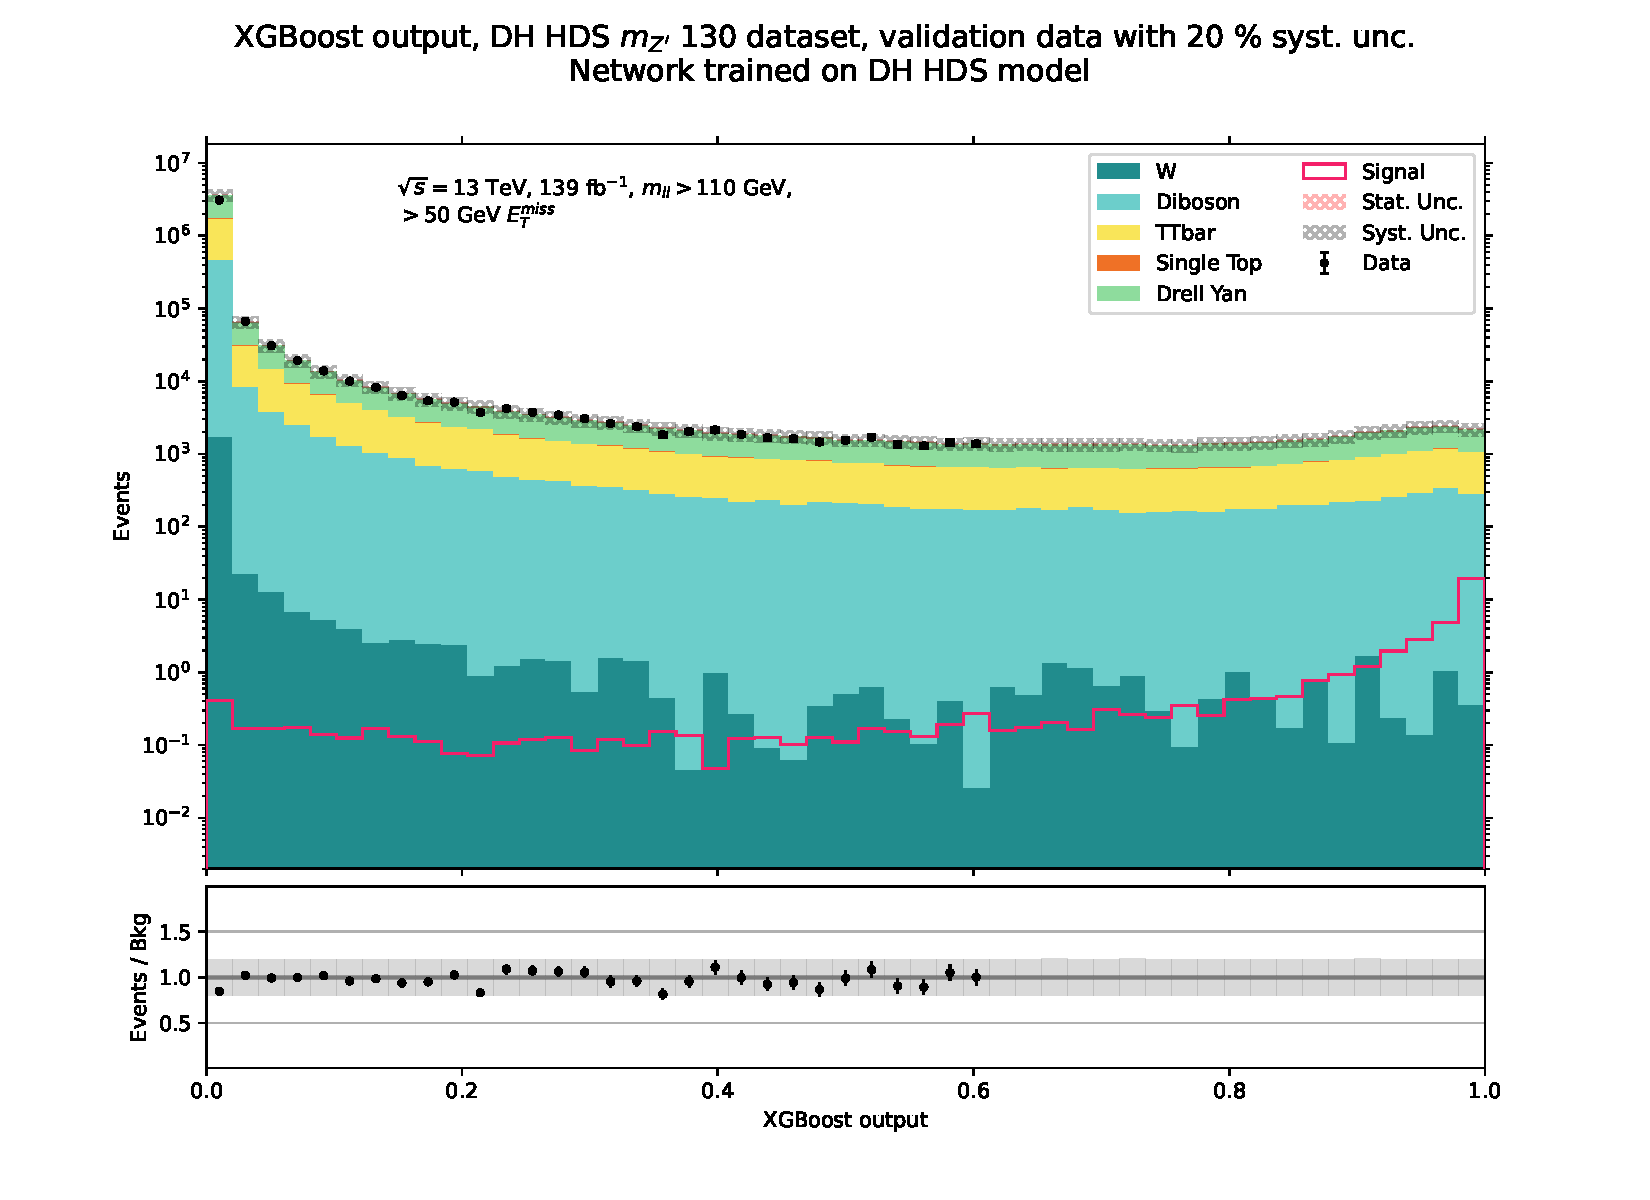
\includegraphics[width=1\textwidth]{Pos_wgt/VAL.pdf}
      \caption{Using only positive weights}
   \end{subfigure}
   \begin{subfigure}[b]{0.49\textwidth}
      \centering
      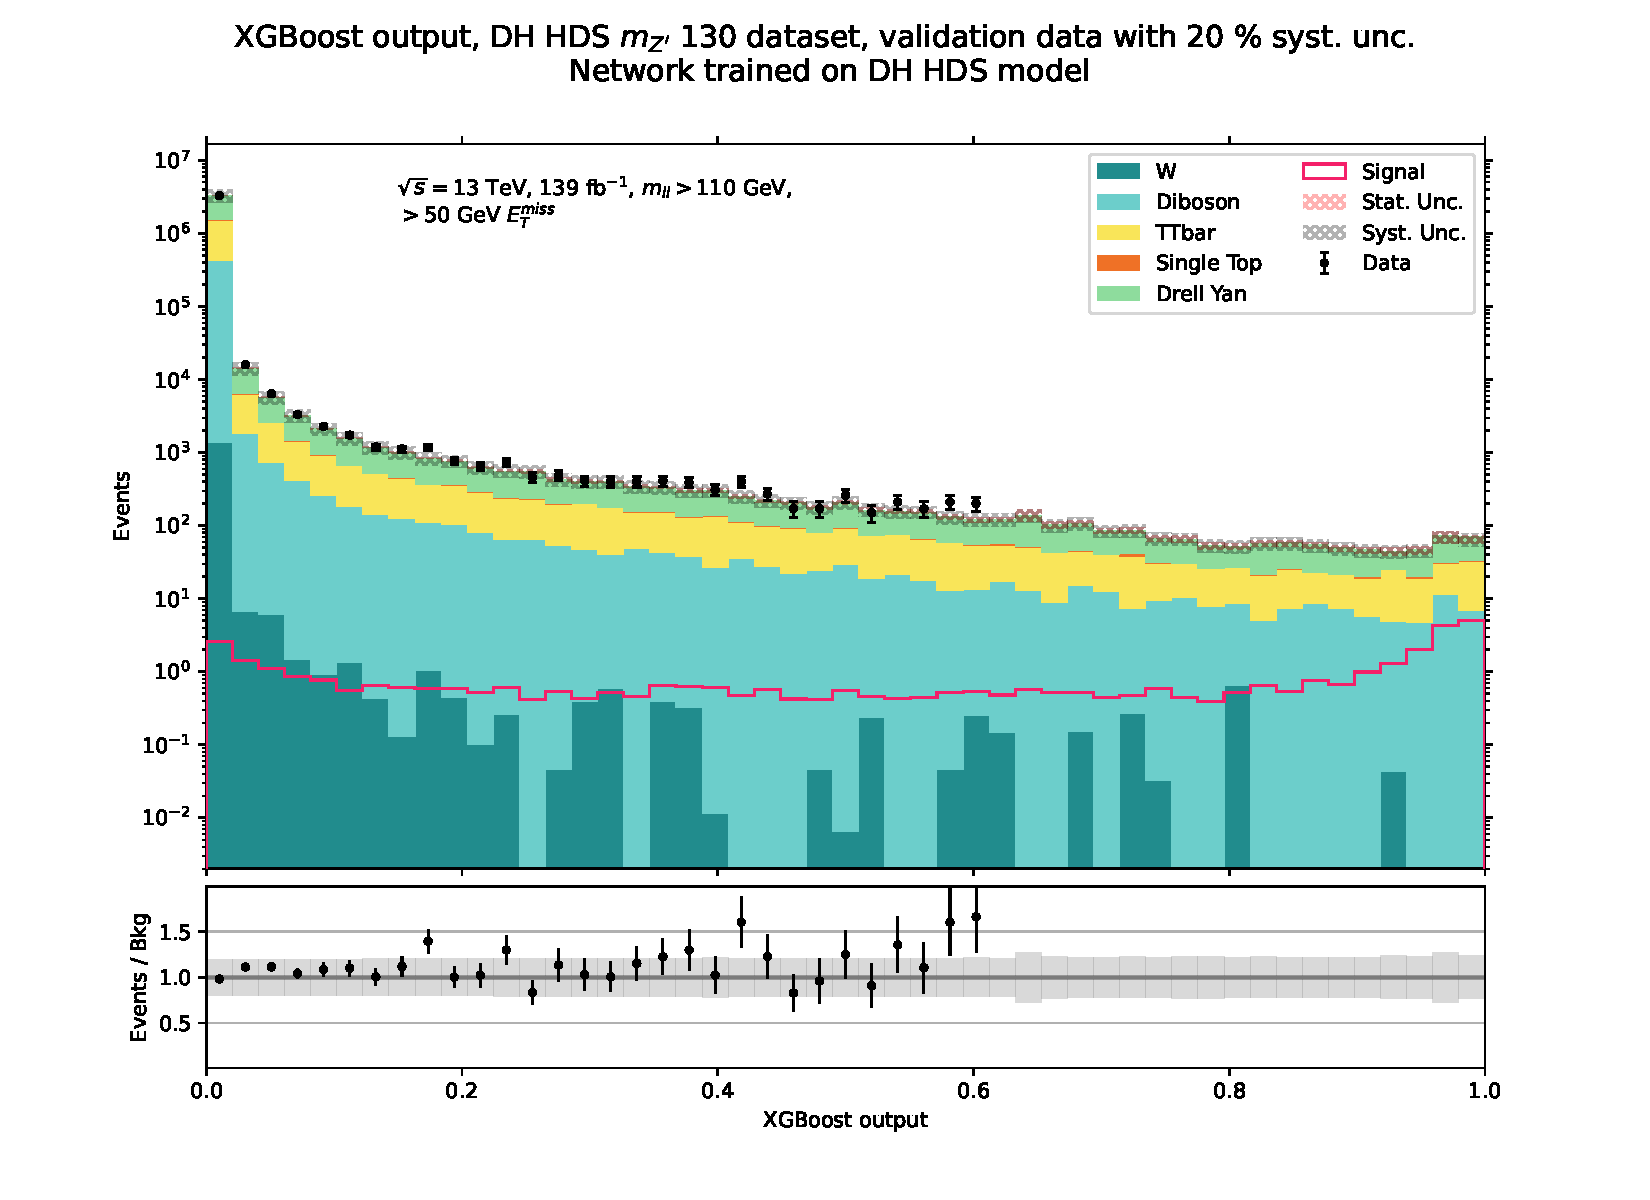
\includegraphics[width=1\textwidth]{No_wgt/VAL.pdf}
      \caption{Using no weights}
   \end{subfigure}
   \caption[Difference when using different weighting methods on BDTs]{Difference when using different weighting methods. All networks were trained using the balancing method explained in Section \ref{sec:bdt_wgts}}\label{fig:BDT_wgts}
\end{figure}
\begin{figure}[!ht]
	\centering
	\begin{subfigure}[b]{0.49\textwidth}
      \centering
      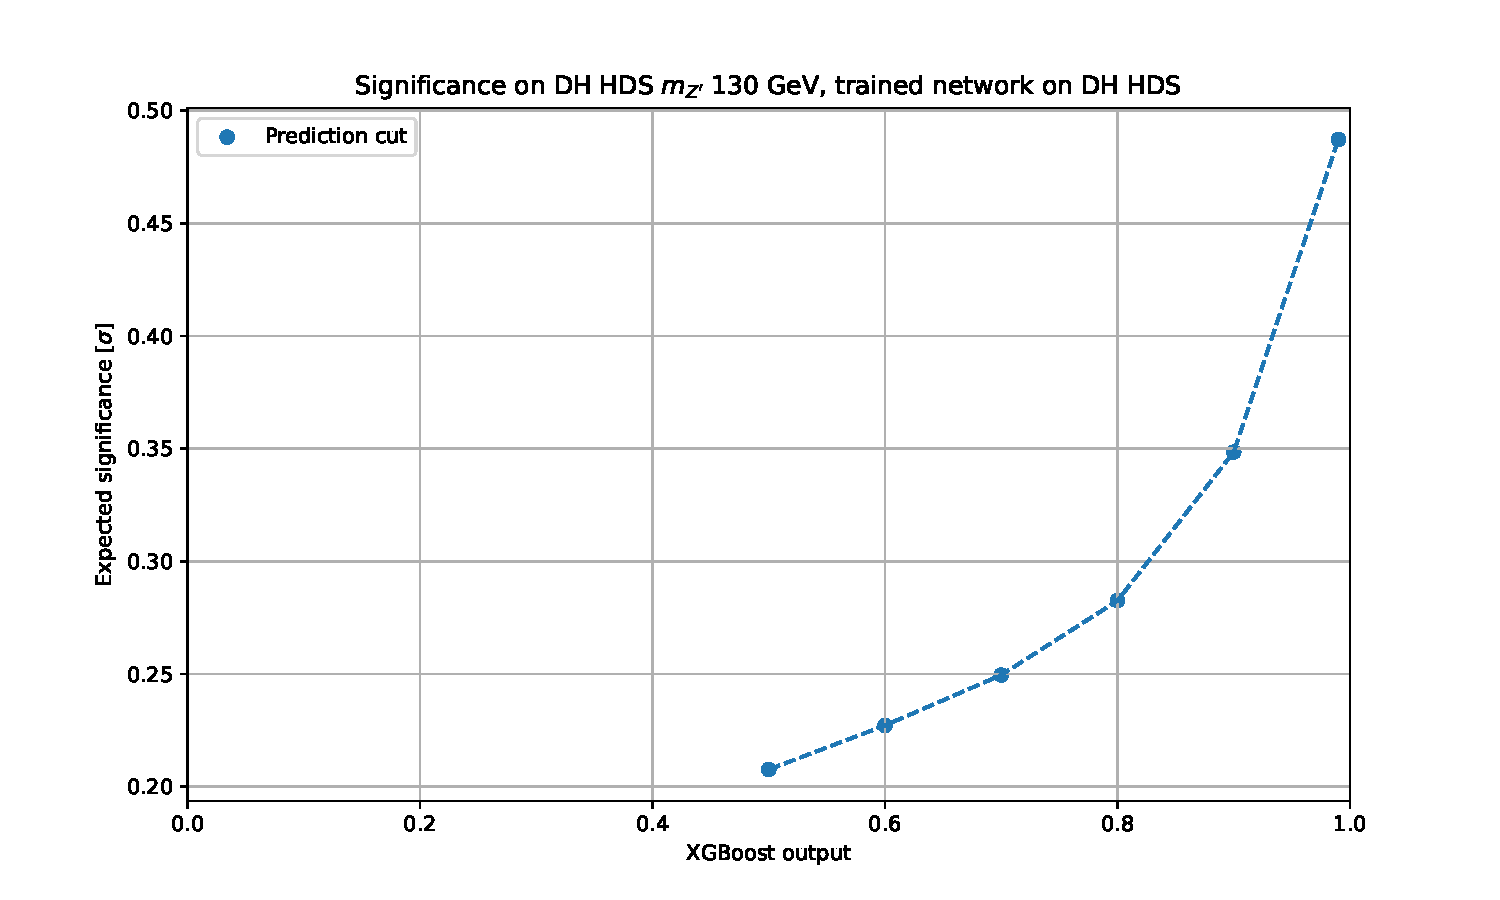
\includegraphics[width=1\textwidth]{Abs_wgt/EXP_SIG.pdf}
      \caption{Using scaled absolute value of weights}
   \end{subfigure}
   \begin{subfigure}[b]{0.49\textwidth}
      \centering
      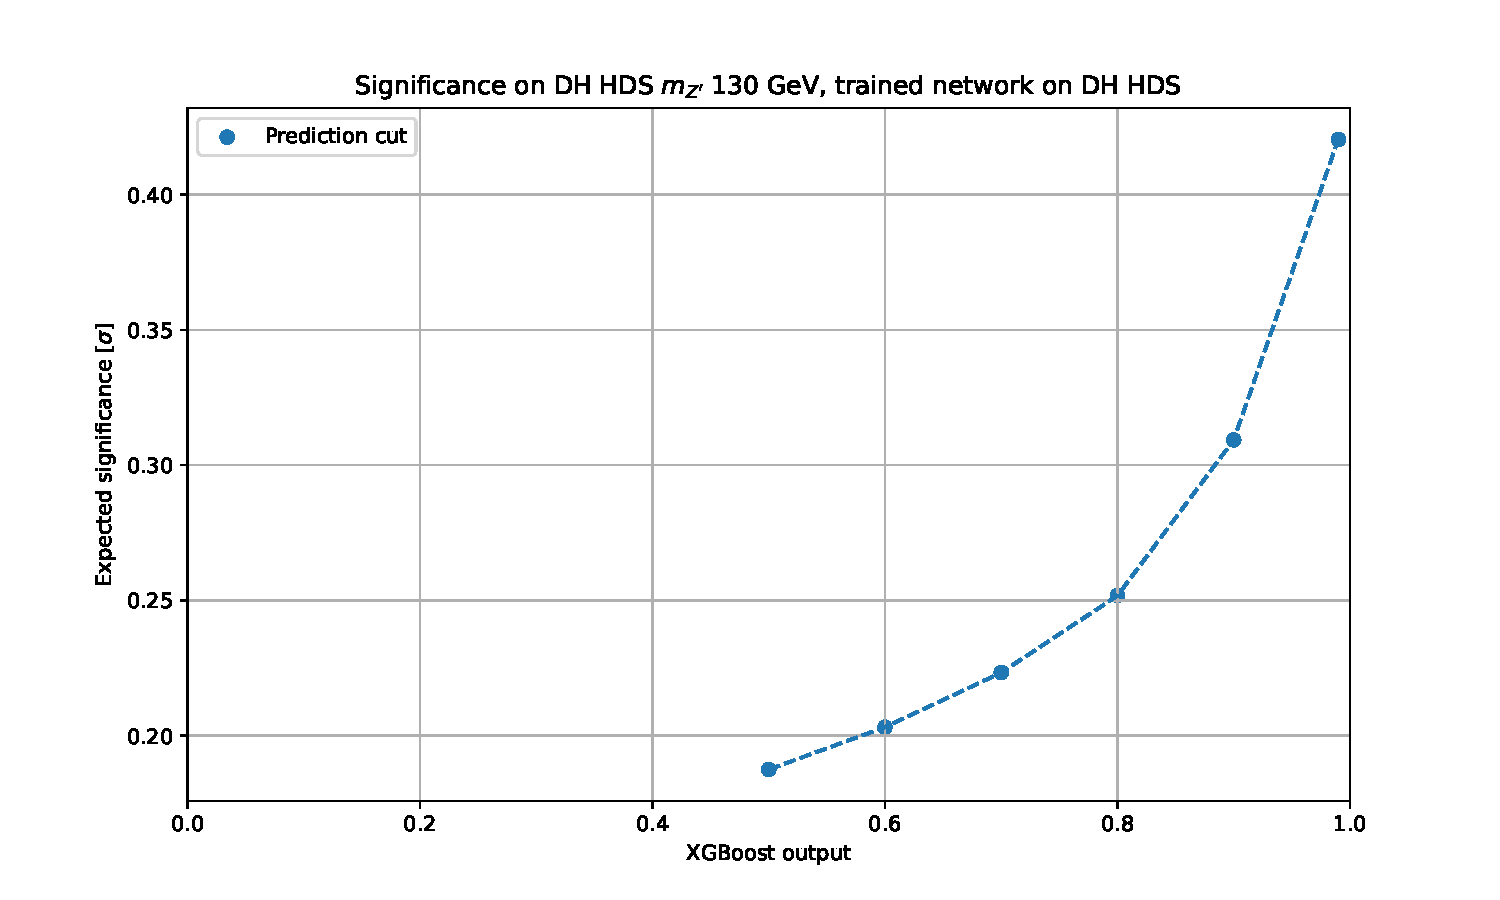
\includegraphics[width=1\textwidth]{Pos_wgt/EXP_SIG.pdf}
      \caption{Using only positive weights}
   \end{subfigure}
   \begin{subfigure}[b]{0.49\textwidth}
      \centering
      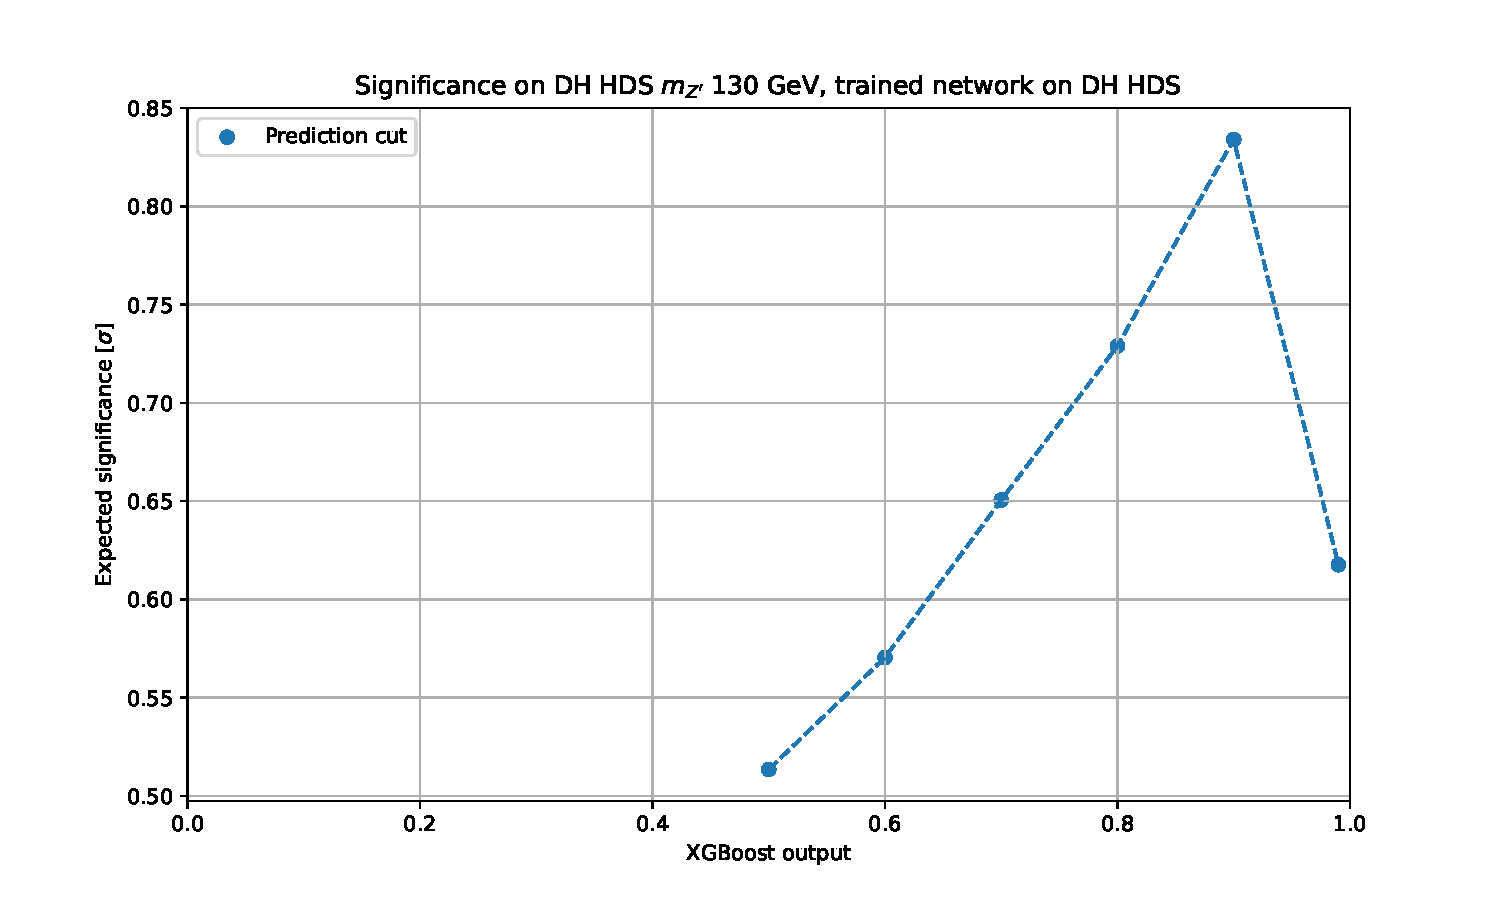
\includegraphics[width=1\textwidth]{No_wgt/EXP_SIG.pdf}
      \caption{Using no weights}
   \end{subfigure}
   \caption[Difference when using different weighting methods on BDTs]{Difference when using different weighting methods. All networks were trained using the balancing method explained in Section \ref{sec:bdt_wgts}}\label{fig:BDT_wgts_sig}
\end{figure}

\clearpage\section{Discussion (draft)}
\todo{Comment on lack of time and DNN thoughts.} 
The last thing to be noted is that having a DNN completely removes the possibility of combining the results of multiple networks trained on a single model, as the imbalance becomes too much for the network to see anything.
A solution to this however, is that instead of combining the results of multiple networks trained on a singular model, one could try the Parametrized NN approach used by Baldi et al. \cite{Baldi_2016}, which could potentially avoid the imbalance problem, but this is 
proposed as a plausible new research project due to time constrain on this thesis.\\
\\\todo{Comment on fully converting to XGBoost.} XGBoost >> TensorFlow


\clearpage
\section{NN algorithm}
\begin{lstlisting}[language=Python, caption={Neural network definition using TensorFlow}, label=alg:nn, captionpos=t]
   import tensorflow as tf
   from tensorflow.keras import layers
   
   def Neural_Network(inputsize, n_layers, n_neuron, eta, lamda):
       
       model=tf.keras.Sequential()      
       
       for i in range(n_layers):       
           if (i==0):                  
               model.add(layers.Dense(n_neuron, activation='relu', kernel_regularizer=
                tf.keras.regularizers.l2(lamda), input_dim=inputsize))
           else:                       
               model.add(layers.Dense(n_neuron, activation='relu', kernel_regularizer=
                       tf.keras.regularizers.l2(lamda)))
                       
       model.add(layers.Dense(1,activation='sigmoid')) 
       
       opt=tf.optimizers.SGD(learning_rate=eta) # or Adam!
       
       model.compile(loss=tf.losses.BinaryCrossentropy(),
                   optimizer=opt,
                   metrics = [tf.keras.metrics.BinaryAccuracy()])
       return model
\end{lstlisting}

\clearpage
\section{BDT algorithm}
\begin{lstlisting}[language=Python, caption={Boosted Decision Tree definition using XGBoost}, label=alg:xgb, captionpos=t]
   import xgboost as xgb
   
   Boosted_Decision_Tree = xgb.XGBClassifier(
                max_depth, 
                use_label_encoder=False,
                n_estimators,
                learning_rate,
                reg_lambda,
                predictor = 'cpu_predictor',
                tree_method = 'hist',
                scale_pos_weight = sow_bkg/sow_sig,
                objective = 'binary:logistic',
                eval_metric = 'auc',
                min_child_weight = 1,
                missing = -999,
                random_state = 42,
                verbosity = 1) 
\end{lstlisting}
\end{document}